%\setlength{\epigraphwidth}{0.5\textwidth}
%\epigraph{There is an art in the contemplation of water. It is necessary to look at it as foaming in waves.}{--- \textup{Mencius}, \textit{\\translated by James Legge}}

The SNO+ water phase data were taken from May 2017 to September 2018. The period from May 2017 to October 2018 is the first stage of the water phase. During this stage, several calibration runs were taken, including the $^{16}$N calibration scans and the laserball scans. During the period from October 2018 to July 2019, over 20 tonnes of LAB (without PPO) was filled into the detector and the LAB mostly occupied the neck volume, slightly below the neck bottom. With the nitrogen cover gas on the top of the AV, the dataset taken during this period is called ``low background dataset''. In this study, 4838 runs of data were used, which summed up a total live time of 190.31 days after the data cleaning process.
 
In this chapter, I applied the MPW reconstruction algorithm described in Chapter 4 as a position and direction fitter to the raw dataset as well as the run-by-run MC simulations. The fitted event vertex was used by the energy fitter developed by the SNO+ collaboration.  

First, the open dataset taken in 2017 was used to test the \texttt{MPW} results, compared to the official RAT results. A quantity called ``Kullback–Leibler Divergence'' was developed to evaluate the Cherenkov signals. After that, I mainly analyzed the low background dataset. I used sub-datasets of the run-by-run MC simulations to evaluate the ability of separating the solar $\nu_e$ signals from the backgrounds. The Toolkit for Multivariate Data Analysis with ROOT (\texttt{TMVA}) package\cite{tmvaWebsite,albertsson2007tmva} was used to train and test on the MC simulations to obtain optimized discriminants. These optimized discriminants were applied on the whole dataset to remove the backgrounds.

The outputs from the data were fitted to obtain the number of signal events and the background events. Ensemble tests were performed on fake datasets to check the fit pull and bias. The systematics obtained from the $^{16}$N calibration in Chapter 5 were applied on the results. Finally, the solar $\nu_e$ interaction rates and the $^8$B solar neutrino flux were evaluated.

%to search for these events then convert into the interaction rate as well as the $^8$B solar neutrino flux.

%Monte Carlo simulations were produced by the RAT software, which was described in \ref{sect:rat}.
%compare to SuperK results.
%data cleaning and analysis cuts 
%The analysis cuts depend on the reconstructed results.
\section{Backgrounds}
\subsection{Physics Backgrounds}

\begin{itemize}
\item Internal backgrounds:

Most backgrounds come from natural radioactive isotopes inside or around the detector, such as the isotopes in the detection medium, detector materials and the PMTs. The major isotopes in the water phase are: $^{238}$U, $^{232}$Th, $^{40}$K, and $^{222}$Rn. These have been monitored by \emph{in-situ} and \emph{ex-situ} measurements and analyses. 

The ubiquitous $^{238}$U and $^{232}$Th isotopes decay sequentially and form decay chains. 
The target level in the SNO+ water phase is $3.5\times 10^{-14}$ gram $^{238}$U in per gram water (gU/gH$_2$O) and $3.5\times 10^{-14}$ gTh/gH$_2$O\cite{waterunidoc}. The rates of the background events caused by the decays from specific isotopes, especially the $\beta$-decays of $^{214}$Bi (from the $^{238}$U decay chain) and $^{208}$Tl (from the $^{232}$Th decay chain), were carefully calculated and were put into the simulations. In this chapter, the simulated background events from the $^{214}$Bi and the $^{208}$Tl $\beta$-decays were used to develop the multi-variable analysis to select solar neutrino events from the background events.

\item External backgrounds:

As mentioned in Chapter 3, Sect.~\ref{sect:overview}, since the depth of the SNO+, the cosmogenic backgrounds induced by the cosmic muons are very few. 
The instrumental backgrounds, such as the flashers from the PMTs, can be removed by the data-cleaning approaches. Here the data-cleaning masks were applied.
\end{itemize}

\section{Kullback–Leibler (KL) Divergence for High Level Cuts}

The Kullback–Leibler (KL) divergence (also called ``relative entropy'') is used to measure the dissimilarity of two probability distributions\cite{murphy2012machine}. I used this quantity to compare the reconstructed angular distribution of an event, $\vec{u}_{fit}\cdot(\vec{X}_{PMT}-\vec{X}_{fit})/|\vec{X}_{PMT}-\vec{X}_{fit}|$, with the angular distribution of solar $\nu_e$ events extracted from the MC (expected as a Cherenkov distribution) to check the dissimilarity of the event compared with the solar $\nu_e$ event. The quantity $D_{KL}(p||q)$ is calculated as: 
\begin{equation}\label{eq:kldiv}
klDiv(p||q) \equiv \sum_{i}^N p(x_i)\log{\frac{p(x_i)}{q(x_i)}},
\end{equation}

where $p(x_i)$ is the angular distribution after a time residual window cut: $-5<t_{Res}<1~ns$, to extract prompt Cherenkov lights. Both of the event and the MC distributions were filled into a histogram with 40 bins ranging from [-1,1] and the $klDiv$ values were calculated bin by bin except the empty bins (zero count). A small $klDiv$ value indicates a small dissimilarity.

These values were used for distinguishing the signal from backgrounds, which will be discussed in the Sect.~\ref{sect:tmva}. Fig.~\ref{kLdiv_example} shows an example of the $klDiv$ calculation. Two events are compared here. One is a randomly selected event from the solar $\nu_e$ run-by-run MC ($E=4.78~MeV$), the other is from the $^{214}$Bi MC ($E=2.18~MeV$), with the same event GTID. It can be seen that the background event with lower energy is more dispersive while the signal event has a peak around the Cherenkov angle ($\sim 0.75$) and thus its shape is more close to the pdf. The calculation of \ref{eq:kldiv} gives $klDiv(solar~\nu_e)=11.78$ and $klDiv(^{214}Bi)=22.69$, which verifies the observation.

\begin{figure}[!htb]
	\centering
	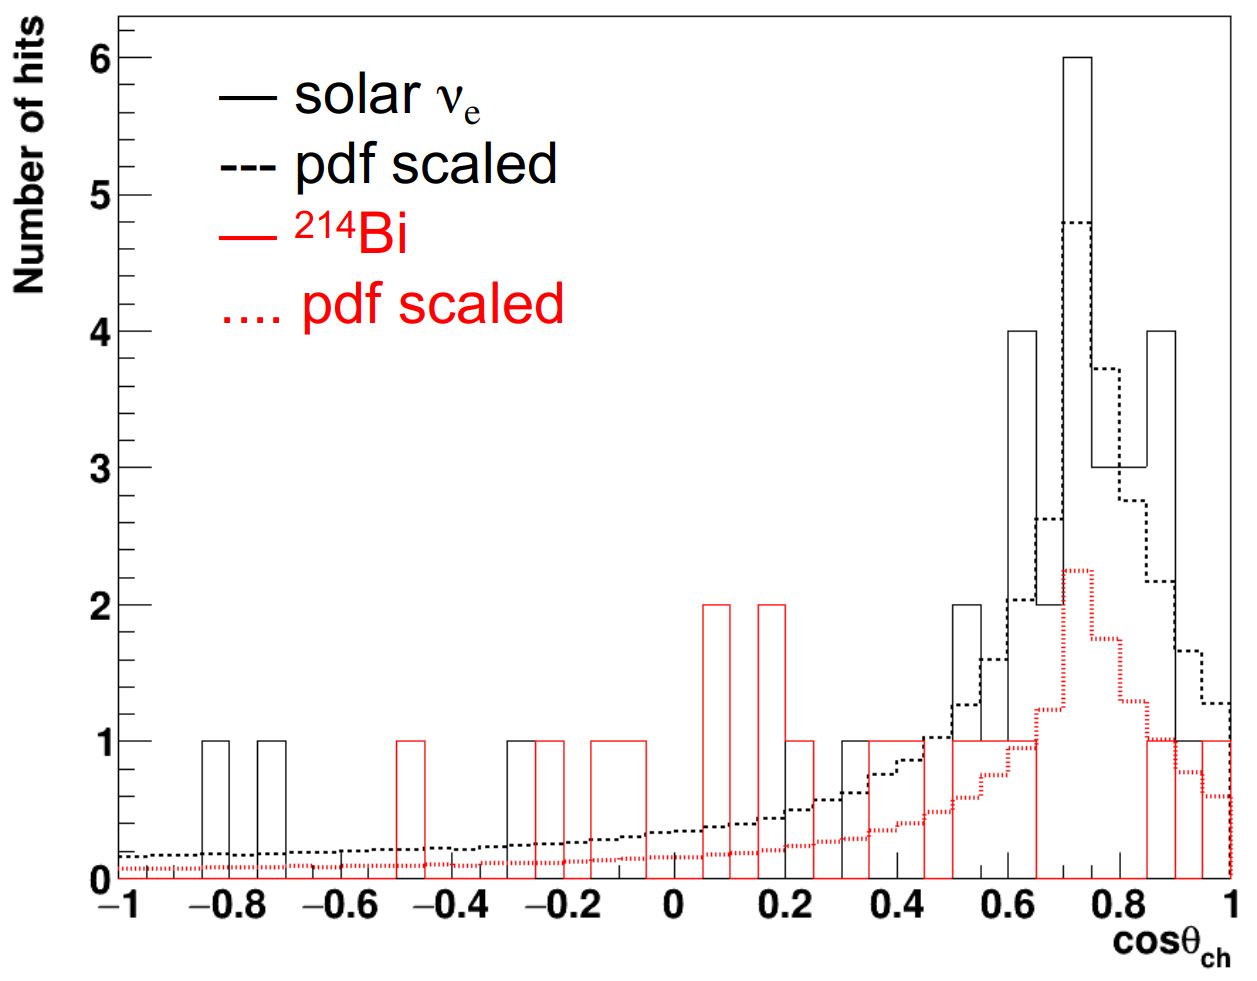
\includegraphics[width=8cm]{klDiv_example.png}
	\caption[Angular distributions of the MC events in run-by-run simulations.]{Angular distributions of the MC events in run-by-run simulations of run-206391, with the same event GTID =7. The black line is the MC solar $\nu_e$ distribution, while the red line is the MC $^{214}$Bi distribution. The $PDF$ is scaled to the number of the hits in solar $\nu_e$ event (black dashed line) and the $^{214}$Bi event (red dotted line) respectively.}
	\label{kLdiv_example}
\end{figure}

A symmetrical form of $klDiv$ can be taken as:
\begin{equation}\label{eq:symKlDiv}
klDiv(p,q) \equiv \frac{1}{2}\sum_{i}^N (p\log{\frac{p}{q}}+q\log{\frac{q}{p}}),
\end{equation}
Since $klDiv(p,q)=klDiv(q,p)$, it has a meaning of distance. This quantity is used in the TMVA method in Sect.~\ref{sect:tmva}.

\section{Solar \texorpdfstring{$\nu_e$}{Lg} Analysis and Background Separation in Water Phase}
\subsection{Open Dataset Analysis}
This open dataset was used to compare the reconstructed events by the \texttt{MPW fitter} and the \texttt{RAT water fitter}.

In SNO+ water phase, solar $\nu_e$s are measured via elastic scattering $\nu_e+e^-\to \nu_e+e^-$ ($\nu+e^-$ ES) (was discussed in Sect.~\ref{sect:nuInteraction}). The observable quantity is the solar angle $\theta_{sun}$, the direction of the event relative to the Sun's location, which is defined as:
\begin{equation}
\cos\theta_{sun}\equiv \vec u_{event}\cdot \frac{\vec{X}_{event}-\vec{X}_{sun}}{|\vec{X}_{event}-\vec{X}_{sun}|},
\end{equation}
where $\vec{X}_{sun}$ is taken as the Sun's location relative to the SNOLAB location since the whole lab can be treated as a point regarding the long distance to the Sun. 

High level cuts mentioned in \ref{sect:high_level_cuts} were applied.

\begin{table}[ht]
	\centering
	\caption[Candidate events in the open dataset.]{Candidate events in the open dataset. Compared the fitted results of the candidate events with different fitters.}
	\label{opendata}
	\begin{tabular*}{150mm}{c@{\extracolsep{\fill}}cccccccc}
		\toprule
		Fitter &	Run &  GTID &  $z-0.108$(m) & $R$(m)& $(R/R_{av})^3$ & $\cos\theta_{sun}$ & SNO+ Day\\
		\hline 
		Rat & 100093 &11108354 &3.49 &3.57 &0.21 &-0.954 &2683.92 \\	
		MPW &  --& --& 3.43 &	3.52 &	0.20	& -0.906 & --\\
		Rat &	100207 &5079885 &-2.61 &4.60 &0.45 &0.816 &2687.04\\
		MPW &	 --& --& -3.63 & \textbf{7.61} &	2.03 & \textbf{0.656} & -- \\
		Rat &100632 &7882360 &1.77 &3.19 &0.15 &0.937 &2696.93\\
		MPW &    --& --&  1.67 & 3.11 &	0.14 & 0.911 & -- \\
		Rat &100663 &15767175 &-4.33& 4.96 &0.56 &0.978 &2698.18\\
		MPW & --& -- &-4.45 &	5.07 &	0.60 &	0.980 & -- \\
		Rat &100915 &169700 &-1.00 &5.10 &0.61 &0.341 &2701.23\\
		MPW &	--& --& -1.08 &	5.08 &	0.61 &	0.337 & -- \\	
		\bottomrule
	\end{tabular*}
\end{table}

\begin{table}[ht]
	\centering
	\caption{Candidate events in the open dataset searched by the \texttt{MPW fitter}.}
	\label{opendataMPW}
	\begin{tabular*}{150mm}{c@{\extracolsep{\fill}}cccccccc}
		\toprule
		Run & GTID & energy & $z-0.108$ & $R$ & $(R/R_{av})^3$ & $\cos\theta_{sun}$\\
		\hline 
		100093 &	11108354	&5.827 & 3.43 & 3.52 & 0.20 & -0.907005\\
		100632&	7882360    &6.183& 1.67 &3.11 &0.14 &0.914612\\
		100663&	15767175   &	6.182 & -4.45 &5.07 &0.60&	0.9807349\\
		100915&	169700   &	5.684 &	-1.07 &5.08 &0.61&0.338534\\
		100984&	8621621&	5.701 & 0.76 &4.75 &0.502&-0.647735\\
		101075&	11673714&	5.667 &4.43 &5.18 &0.64& 0.587303\\
		\bottomrule
	\end{tabular*}
\end{table}

A plot of refitting the candidate solar events from the \texttt{Rat water fitter} with the \texttt{MPW fitter} on open dataset.
\begin{figure}[htbp]
	\centering
	\subfigure[Run 100093, GTID 11108354]{ 
		\begin{minipage}[t]{0.4\textwidth}
			\centering
			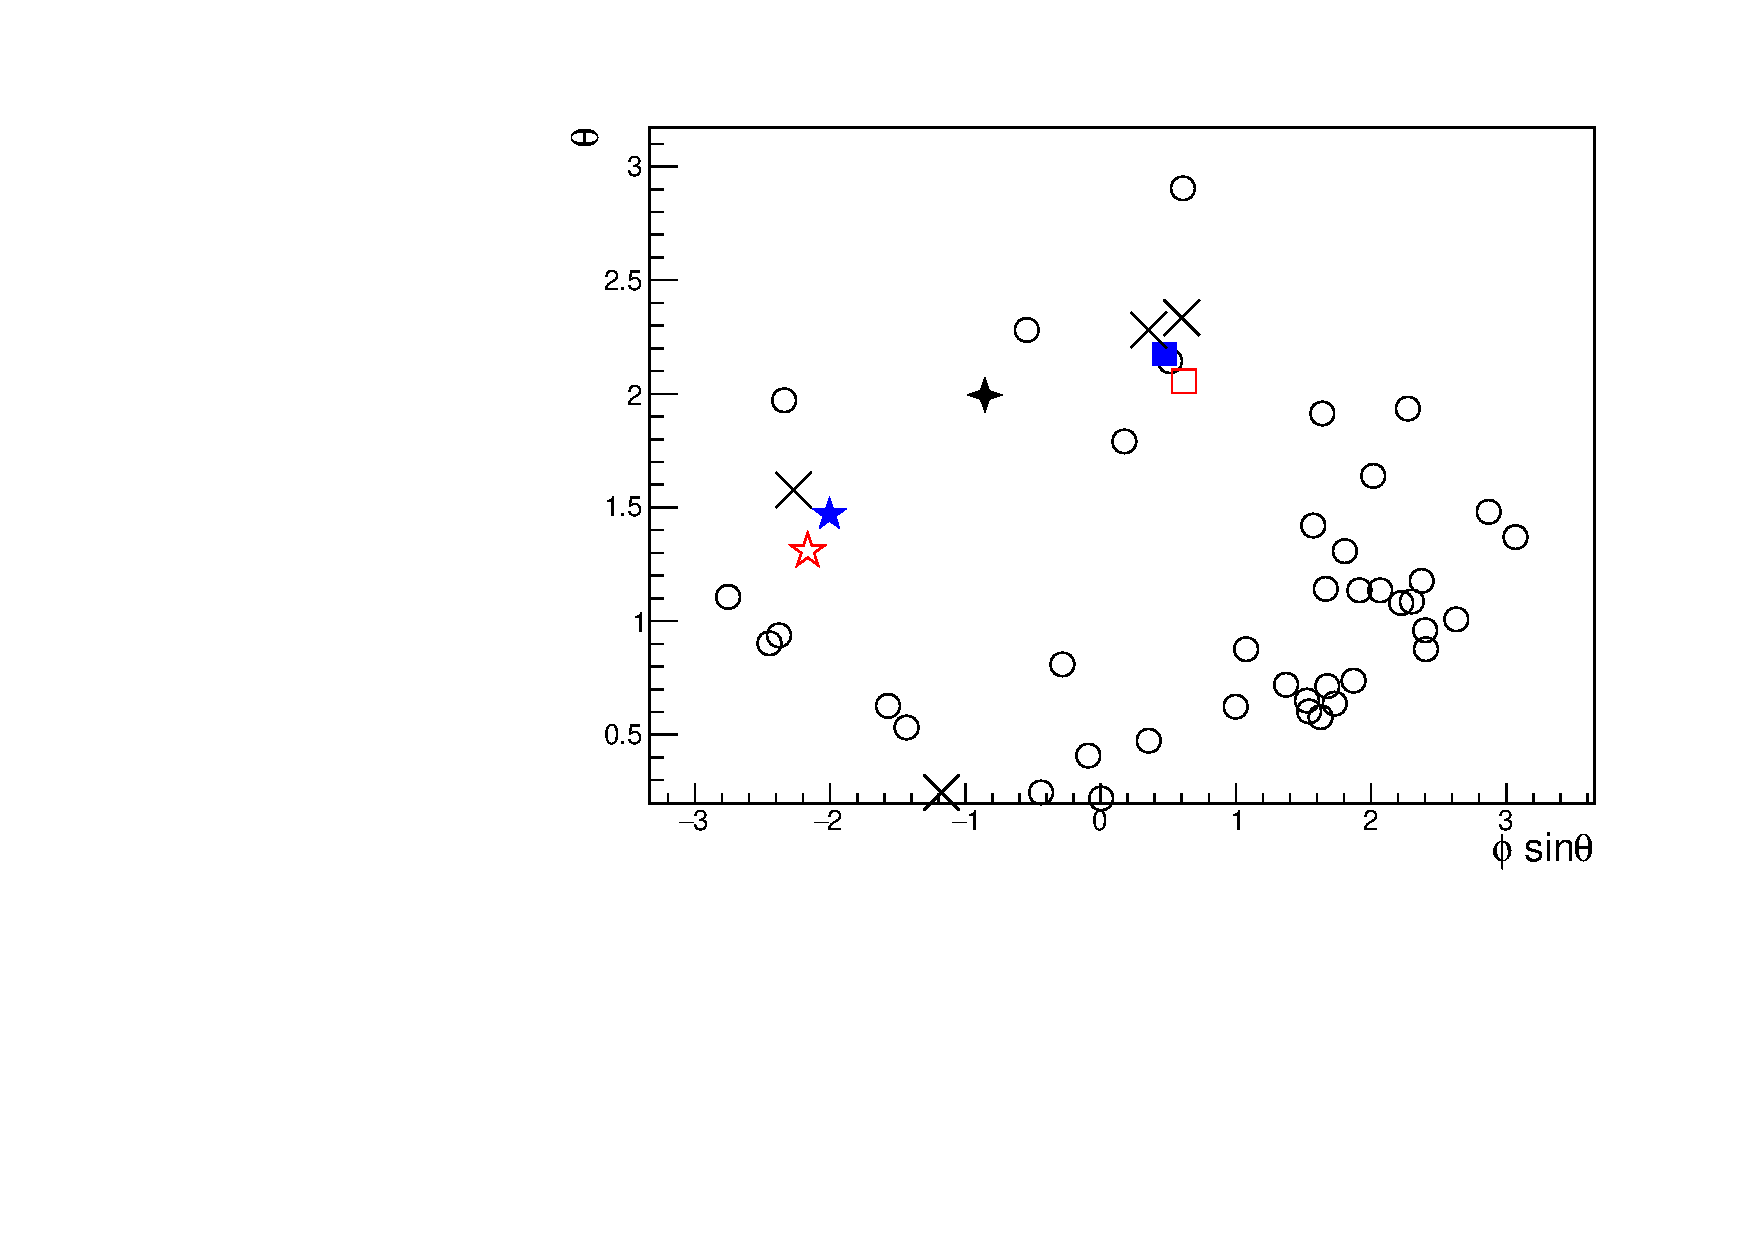
\includegraphics[width=6cm]{PMTmap_100093.pdf}
		\end{minipage}
	}
	\subfigure[Run 100207, GTID 5079885]{ 
		\begin{minipage}[b]{0.4\textwidth}
			\centering
			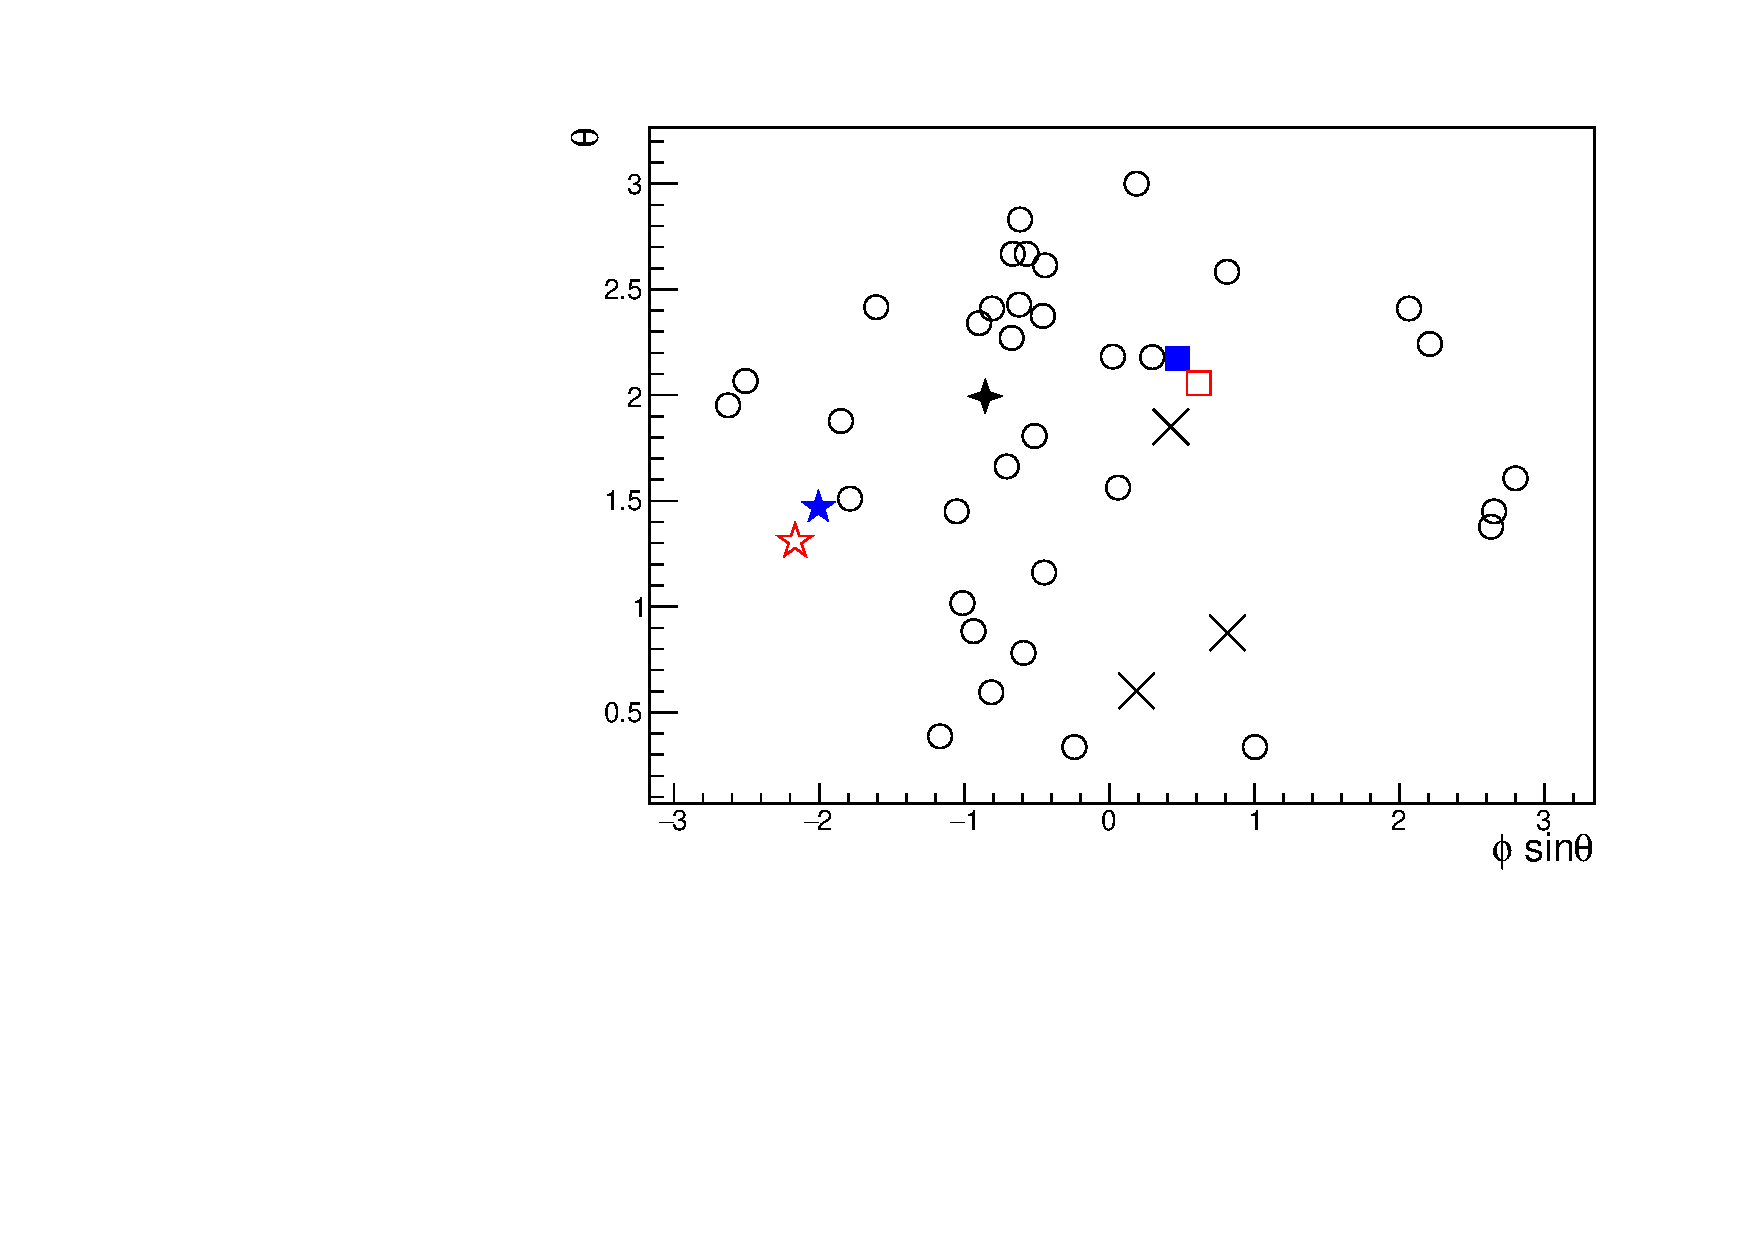
\includegraphics[width=6cm]{PMTmap_100207.pdf}
		\end{minipage}
	}
	\subfigure[Run 100632, GTID 7882360]{ 
		\begin{minipage}[t]{0.4\textwidth}
			\centering
			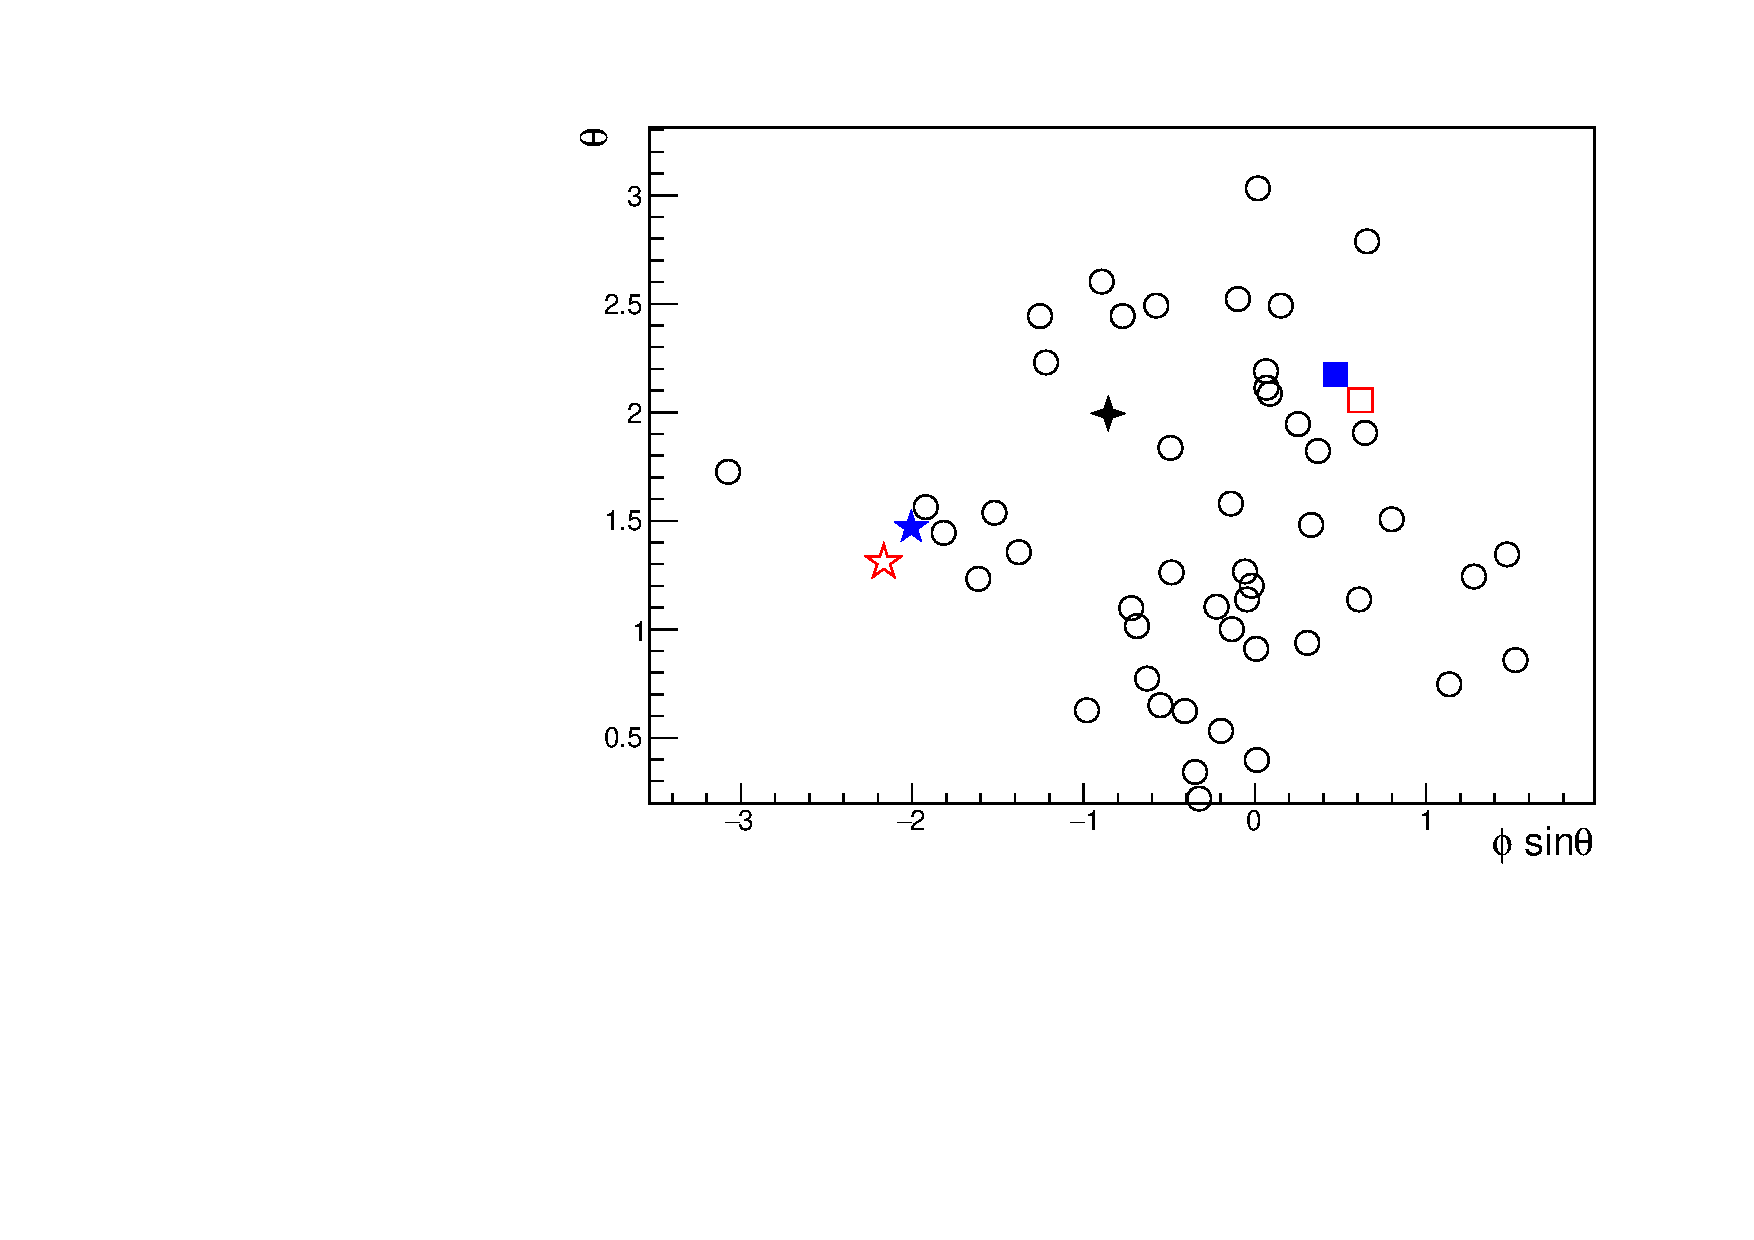
\includegraphics[width=6cm]{PMTmap_100632.pdf}
		\end{minipage}
	}
	\subfigure[Run 100663, GTID 15767175]{ 
		\begin{minipage}[t]{0.4\textwidth}
			\centering
			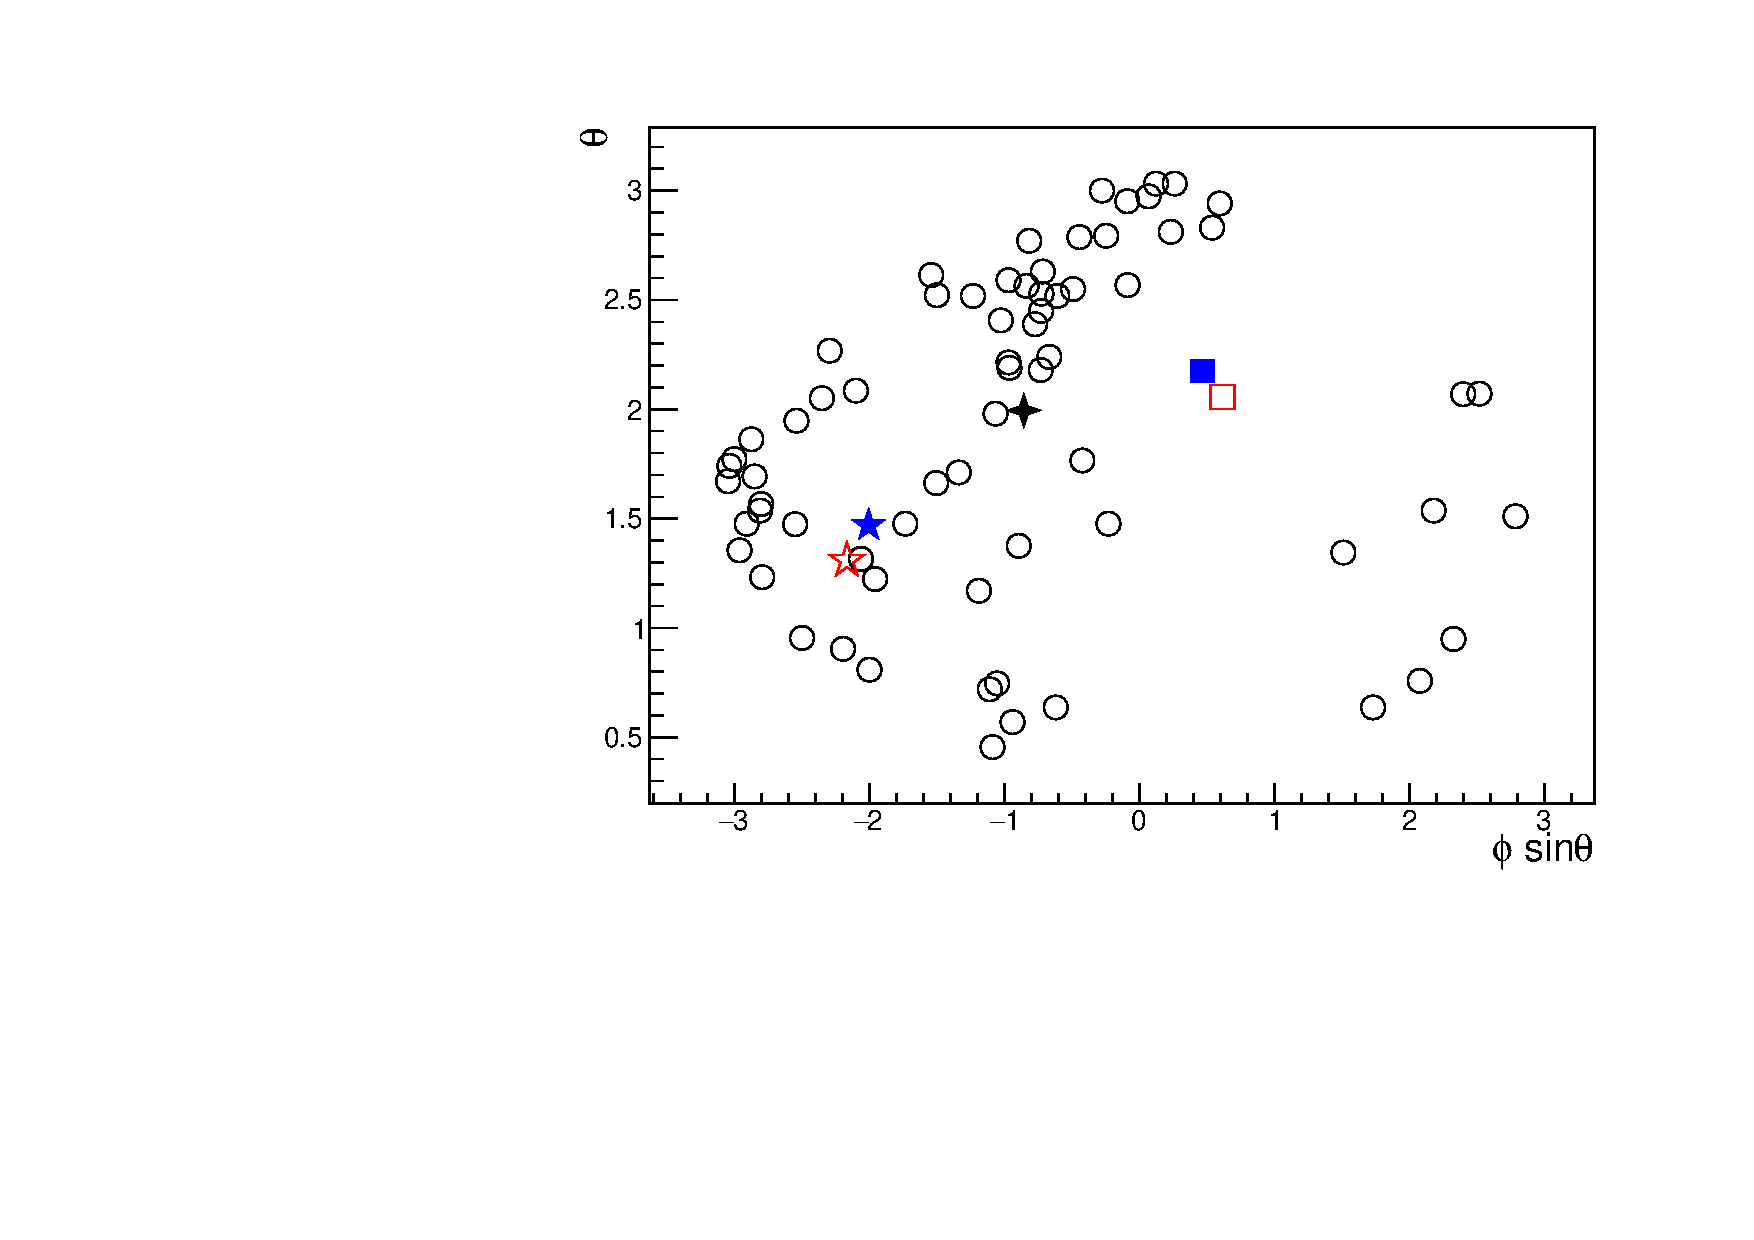
\includegraphics[width=6cm]{PMTmap_100663.pdf}
		\end{minipage}
	}
	\subfigure[Run 100915, GTID 169700]{ 
		\begin{minipage}[t]{0.4\textwidth}
			\centering
			{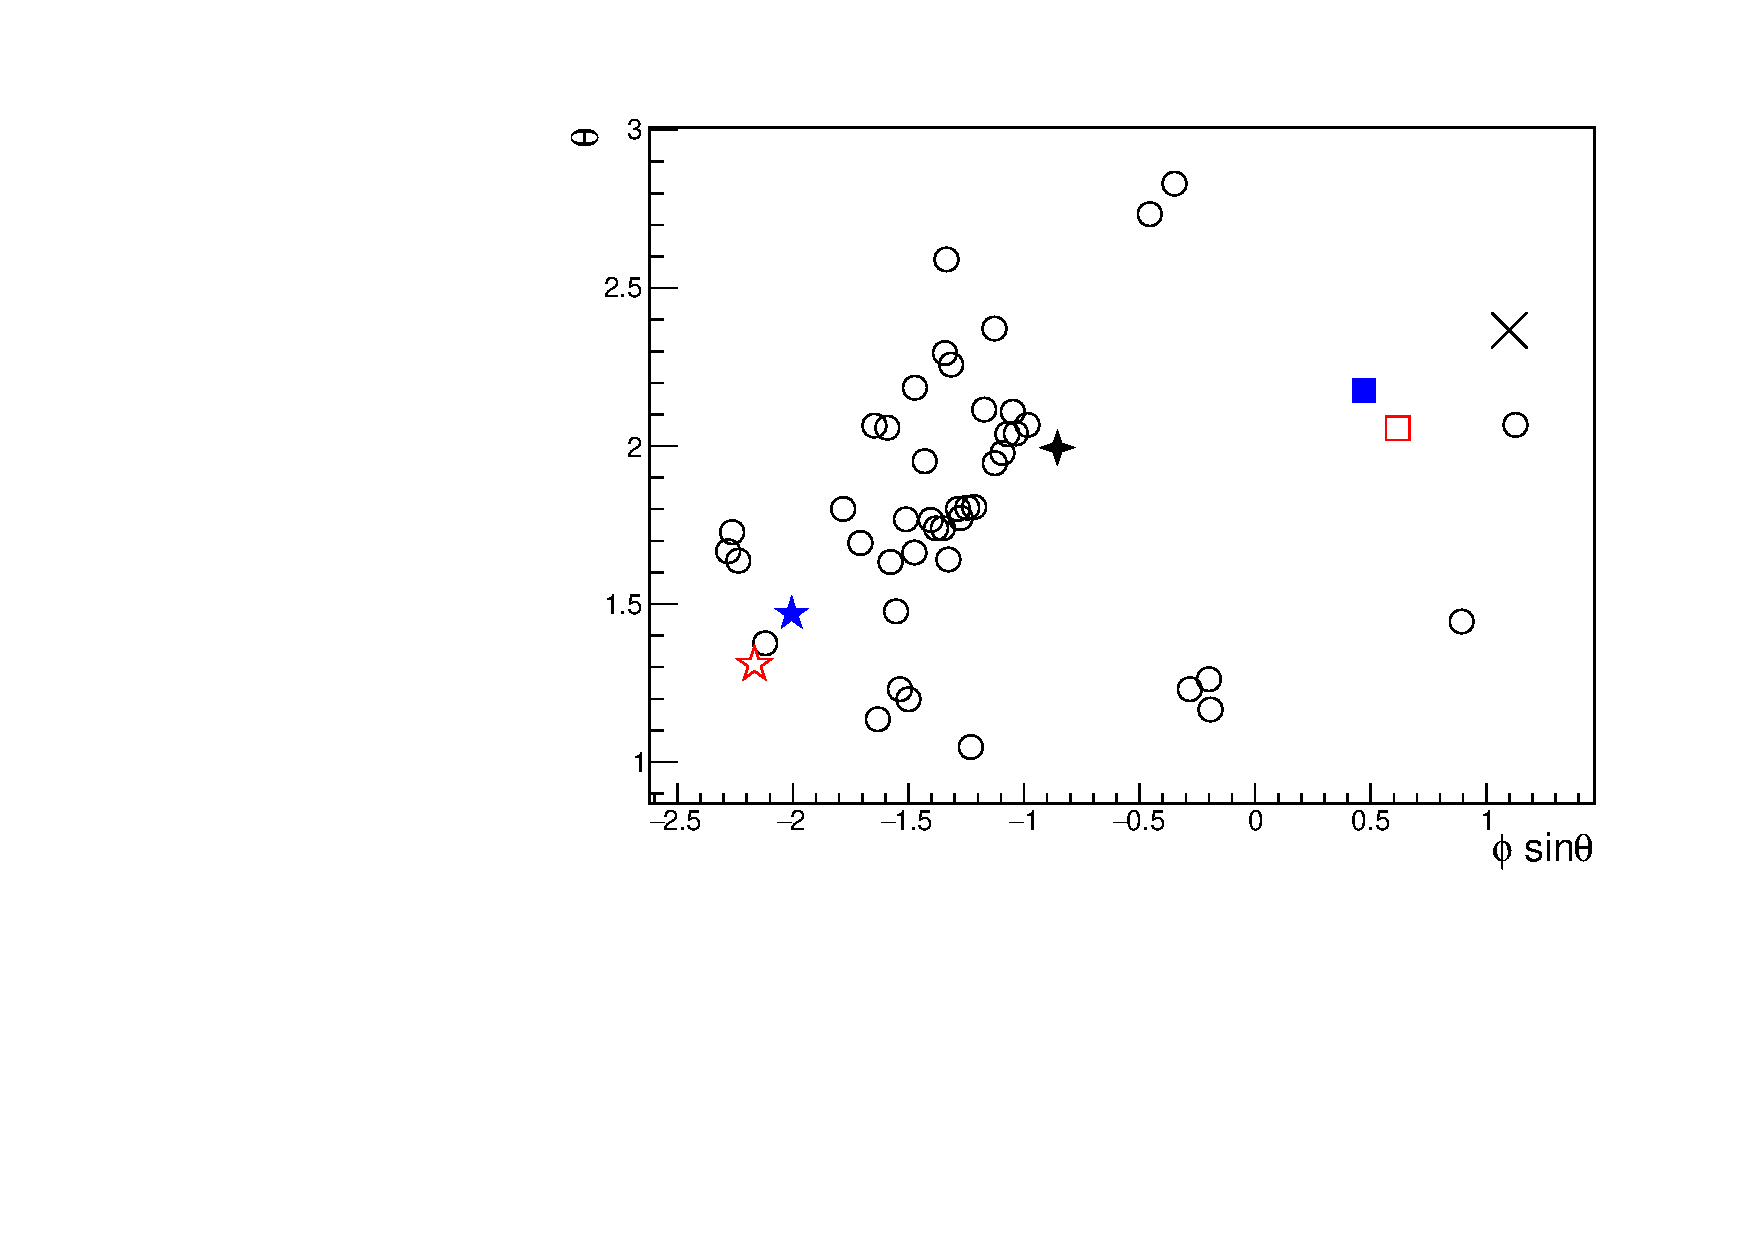
\includegraphics[width=6cm]{PMTmap_100915.pdf}}
		\end{minipage}
	}
	\subfigure[Legends]{ 
		\begin{minipage}[b]{0.4\textwidth}
			\centering
			{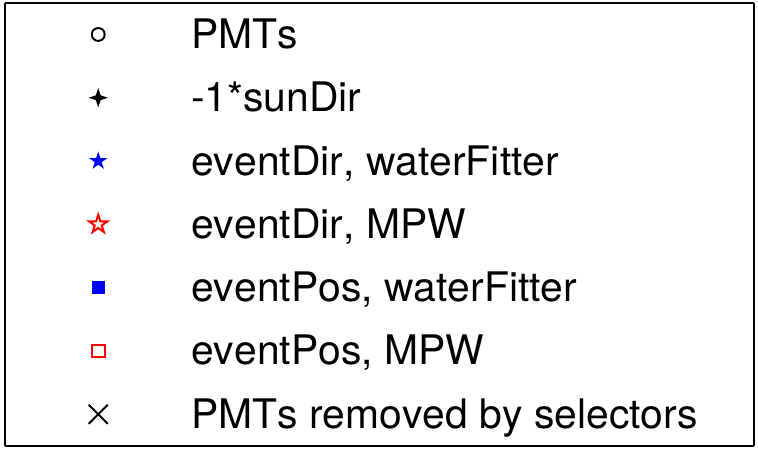
\includegraphics[width=5cm]{solarLegends.png}}
		\end{minipage}
	}
	\caption[Reconstruction results for the candidate events, projected onto PMT sinusoidal maps.]{Reconstruction results for the candidate events, projected onto PMT sinusoidal maps. Black circles stand for
		the hit PMTs used by the fitter; crosses stand for the hit PMTs removed by the selectors; blue full star stands for the event direction fitted by the \texttt{Rat water fitter}; red open star stands for the direction fitted by the \texttt{MPW fitter}; full double diamond stands for the solar direction*-1; blue full square stands for the event position fitted by the \texttt{Rat water fitter}; open square stands for the position fitted by the \texttt{MPW fitter}.}
	\label{openDataSetCandidate}
\end{figure}

% Compare the $klDiv$ quantities for the \texttt{MPW fitter} and \texttt{Rat water fitter} results. 

\subsection{Signal-background Discrimination Based on TMVA}\label{sect:tmva}
This section describes a signal-background discrimination analysis based on the TMVA method. Here the run-by-run simulations that simulated the full detector conditions for a specific run were used. The MC dataset includes the run-by-run simulations from the run-200004 to 203602, which has a live time of 92.54 days and is about a half of the whole ``low background dataset''. Thus it is denoted as the ``half dataset''. This half dataset was used for testing the analyses in this section and the next.

For the MC dataset, two types of background isotopes, $^{208}$Tl and $^{214}$Bi were simulated in different detector regions. In this study, the background events simulated in the inner AV (internal backgrounds) , in the AV and in the external water region were checked. The solar $\nu_e$ events simulated in the inner AV were used as signals. Table.~\ref{table:mixed_MC} summarizes the types of simulations used in this study. 
\begin{table}[ht]
	\centering
	\caption{Datasets of MC simulations.}
	\label{table:mixed_MC}
	\begin{tabular*}{100mm}{c@{\extracolsep{\fill}}cccccccc}
		\toprule
		Simulations & Simulated positions in the detector\\
		\hline 
		$^{208}$Tl & inner AV (internal $^{208}$Tl)\\
		-- & AV \\
		-- & external water (external $^{208}$Tl)\\
		\midrule
		$^{214}$Bi & inner AV (internal $^{214}$Bi)\\
		-- & AV \\
		-- & external water (external $^{214}$Bi)\\
		\midrule
		Solar $\nu_e$ & inner AV (internal $\nu_e$)\\
		-- & AV \\
		-- & external water (external $\nu_e$)\\
		\bottomrule
	\end{tabular*}
\end{table}

Different types of the simulations were merged into a mixed dataset. The simulated solar $\nu_e$ events are tagged as signals and mixed with $^{214}$Bi and $^{208}$Tl background events. The total dataset was divided into training and testing sets. 

Fig.~\ref{TMVA_bkgs_1} shows the energy spectrum of simulated internal events with their fitted positions inside the 5.5-m fiducial volume, i.e., with a radial cut of $R'_{fit}<5.5$~m, where the $R'_{fit}$ is the magnitude of the reconstructed event position $\vec{X}_{fit}$ after the AV coordinate correction: $R'_{fit}\equiv\sqrt{x^2_{fit}+y^2_{fit}+(z_{fit}-108)^2}$. The 108 mm offset in $z$ was discussed in Chapter 3 and Chapter 4. 

\begin{figure}[!htb]
	\centering
	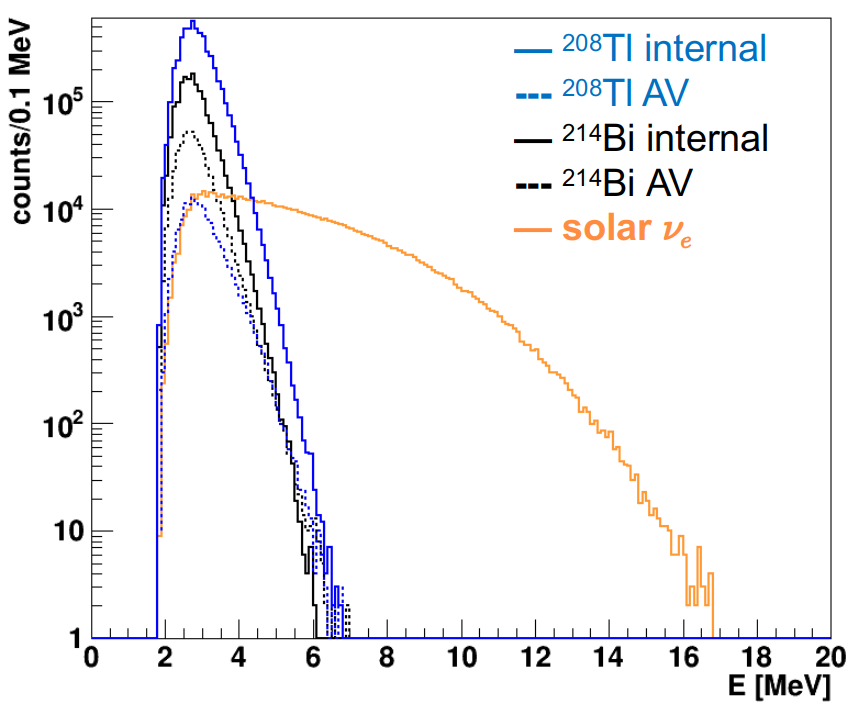
\includegraphics[width=8cm]{TMVA_bkgs_1.png}
	\caption[Energy spectrum of events from different simulations.]{Energy spectrum of events from different simulations in the half dataset: $^{214}$Bi (black), $^{208}$Tl (blue) and solar $\nu_e$ (orange). Solid lines show the internal events and dotted lines show the AV events.}
	\label{TMVA_bkgs_1}
\end{figure}

In the MC dataset, runs from run-200004 to 202516 were taken as the training set (about 67 live days and 72.4\% of the half dataset), and the rest 27.6\% were taken as testing set\footnote{For a more unbiased analysis, a bootstrap method\cite{murphy2012machine} that randomly separates the training and testing datasets can be used, but it is not applied here.}. Once the weights of the variables were obtained by the TMVA training, the weights were applied to the actual data.

Before the analysis, a few ``beforehand cuts'' were applied: NHits$>20$, $R'_{fit}<5500~mm$, $ITR>0.55$, and $-0.12<\beta_{14}<0.95$. Here NHits$>20$ is a reconstruction threshold set for the solar neutrino analysis, which means that only the events with NHits$>20$ were reconstructed by the \texttt{MPW fitter}; the default fiducial volume is $5500$ mm; the $ITR$ and $\beta_{14}$ cuts were suggested by the collaboration, which were mostly based on the experiences for removing the instrumental backgrounds\cite{waterunidoc}. 

Two other ranges of $E_{fit}$ were also tested: $4<E_{fit}<5$ MeV (low energy region) and $5<E_{fit}<15$ MeV ($E>5$ MeV region). 

After applying these beforehand cuts, for the different energy regions, the ratios of the signal event numbers ($N_{sig}$) to the background event numbers ($N_{bkg}$) are listed in Table.~\ref{tab:signalToBkg_tmva}. It shows that, in the low energy region $4<E_{fit}<5$ MeV, the background events are dominant, while for the $E_{fit}>5$ MeV, the background events are significantly reduced.

\begin{table}[ht]
	\centering
	\caption{Ratios of the signal event numbers to the background event numbers.}
	\label{tab:signalToBkg_tmva}
	\begin{tabular*}{100mm}{c@{\extracolsep{\fill}}ccc}
		\toprule
		energy region (MeV) & $N_{sig}$ & $N_{bkg}$ & $N_{sig}/N_{bkg}$ \\
		\midrule
		$4<E_{fit}<15$ & 434830& 166280& 2.6 \\ 
		\midrule
		$5<E_{fit}<15$ & 317205 & 6359 & 49.9\\
		\midrule
		$4<E_{fit}<5$ & 117625 & 159921& 0.73\\
		\bottomrule
	\end{tabular*}
\end{table}

Three classification methods implemented in the TMVA package were applied to the training and testing datasets: the Fisher discriminants/linear discriminant analysis (Fisher/LD), the Boosted Decision Tree (BDT), and the Artificial Neural Networks Multilayer Perceptron (ANN-MLP, or MLP in short)\cite{albertsson2007tmva}.

The Fisher discriminant $y_{F_i}(i)$ for classifying event $i$ is defined by \cite{tmvaWebsite}:
\begin{equation}
y_{F_i}(i) = F_0+\sum_{k=1}^{n_{params}}F_k x_k(i),
\end{equation}
where $n_{params}$ is the number of input variables; the Fisher coefficients, $F_k$ is given by:
\begin{equation}
F_k = \frac{\sqrt{N_SN_B}}{N_S+N_B}\sum_{l=1}^{n_{params}}1/W_{kl}(\bar{x}_{S,l}-\bar{x}_{B,l}),
\end{equation} 
where $N_{S(B)}$ are the number of signal (background) events in the training sample; $\bar{x}_{{S(B),l}}$ are the means of input variables for signal (background); $W_{kl}$ is the covariance matrix\cite{tmvaWebsite}.

For the settings in the TMVA, the BDT method was set with: (1) using the adaptive boosting (AdaBoost) algorithm; (2) training 400 trees with a maximum depth of 3; and (3) using gini index for the decision tree. 

The MLP method was set with: (1) using sigmoid function as the activate function; and (2) using neural networks with 4 hidden layers and 200 training cycles.

There are 9 variables used as the TMVA inputs: $ITR$, $\beta_{14}$, $E_{fit}$, $G_{test}$, $U_{test}$, $scaleLogL$, $Z_{factor}$, $\vec{u}\cdot \vec{R'}$ and $klDiv$ (in the symmetrical form: Eqn.~\ref{eq:symKlDiv}). Among them, the beforehand cuts had been applied to the $ITR$ and $\beta_{14}$, and the $E_{fit}$ had been selected for different regions, as mentioned previously. Here the NHits and $\theta_{ij}$ were not used, since the NHits is correlated to the energy while the $\theta_{ij}$ is anticorrelated to the $\beta_{14}$.

The distributions of these variables are shown in Fig.~\ref{fig:inputParamsTMVA}. The differences between the signal (black solid lines) and background (red dotted lines) distributions can be observed.

\begin{figure}[htbp]
	\centering
	\subfigure[$\beta_{14}$]{
		\begin{minipage}[t]{0.3\textwidth}
			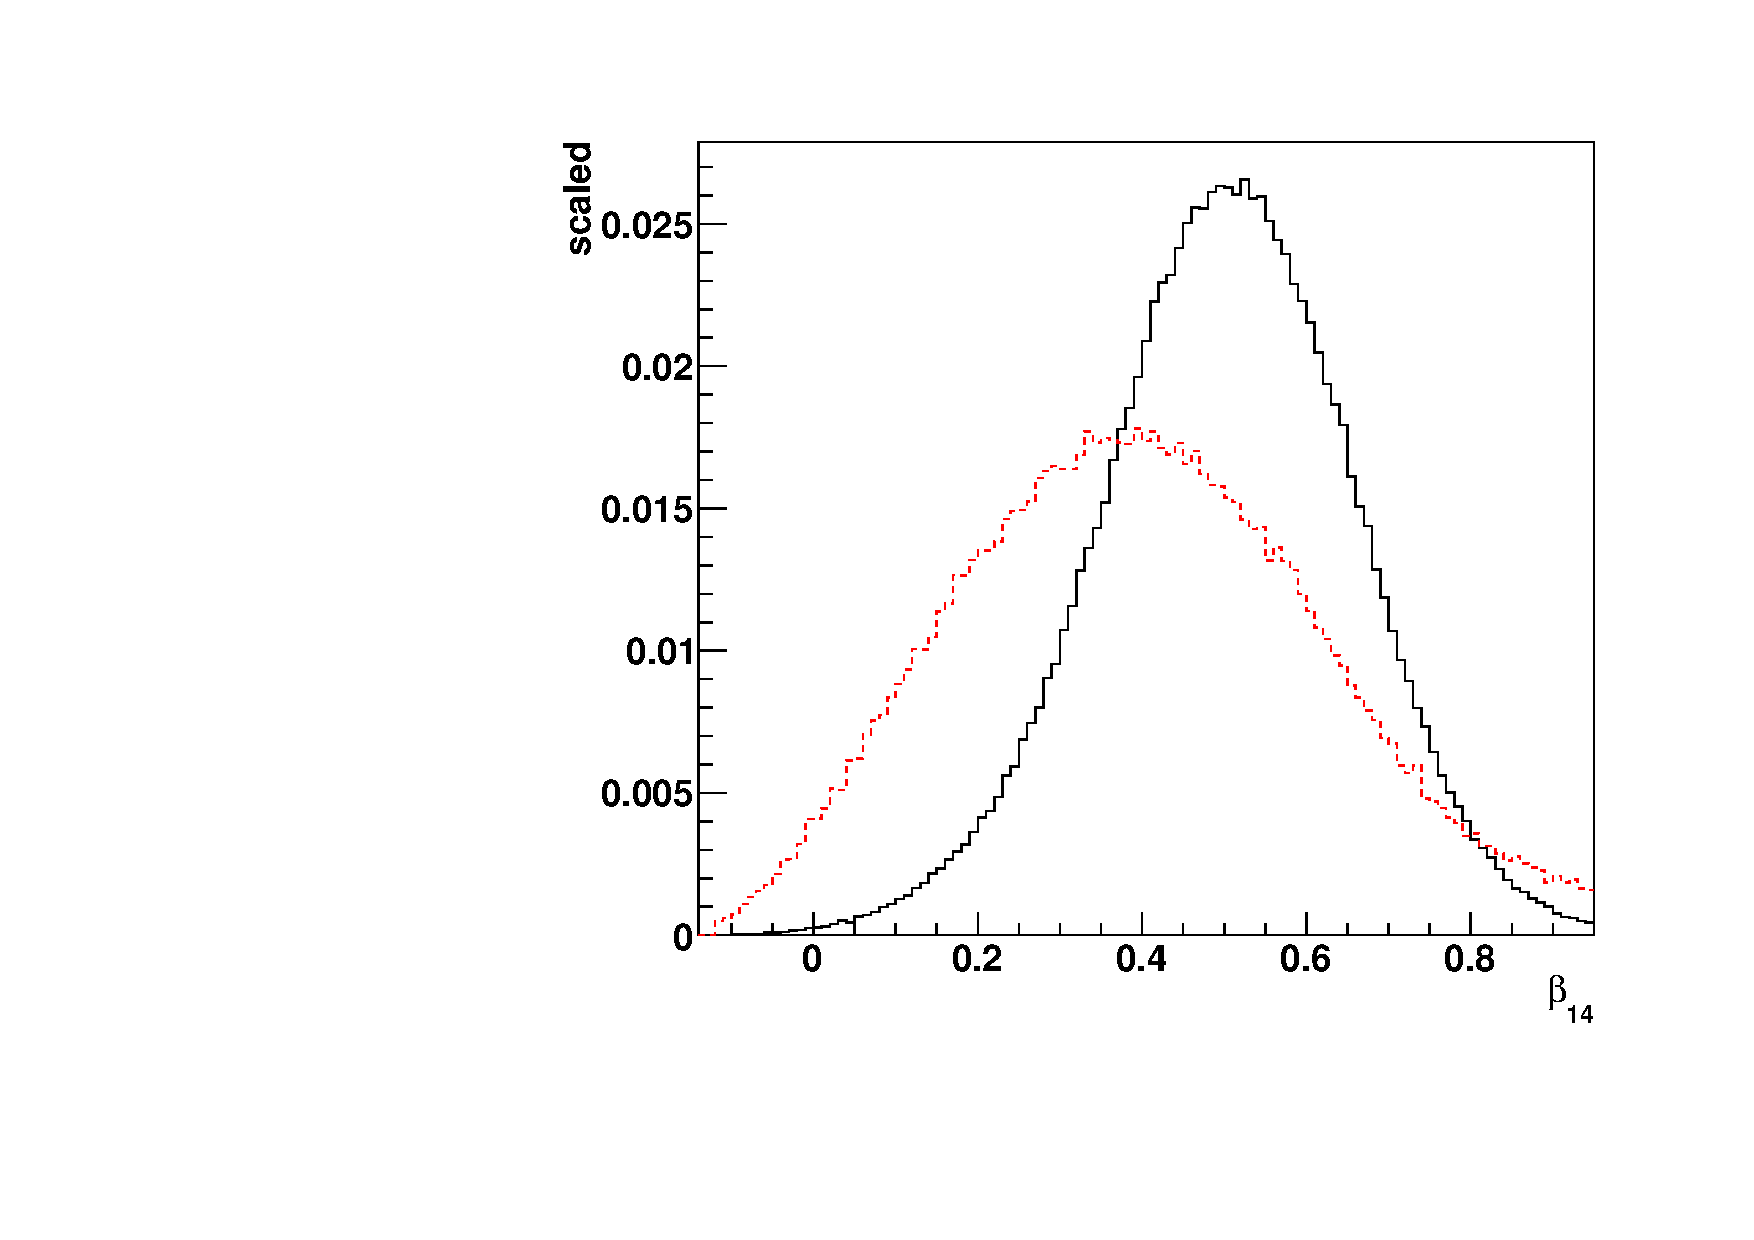
\includegraphics[width=4cm]{tmvaCompare_Beta14.pdf}
		\end{minipage}
	}
	\subfigure[$E_{fit}$]{
		\begin{minipage}[b]{0.3\textwidth}
			\centering
			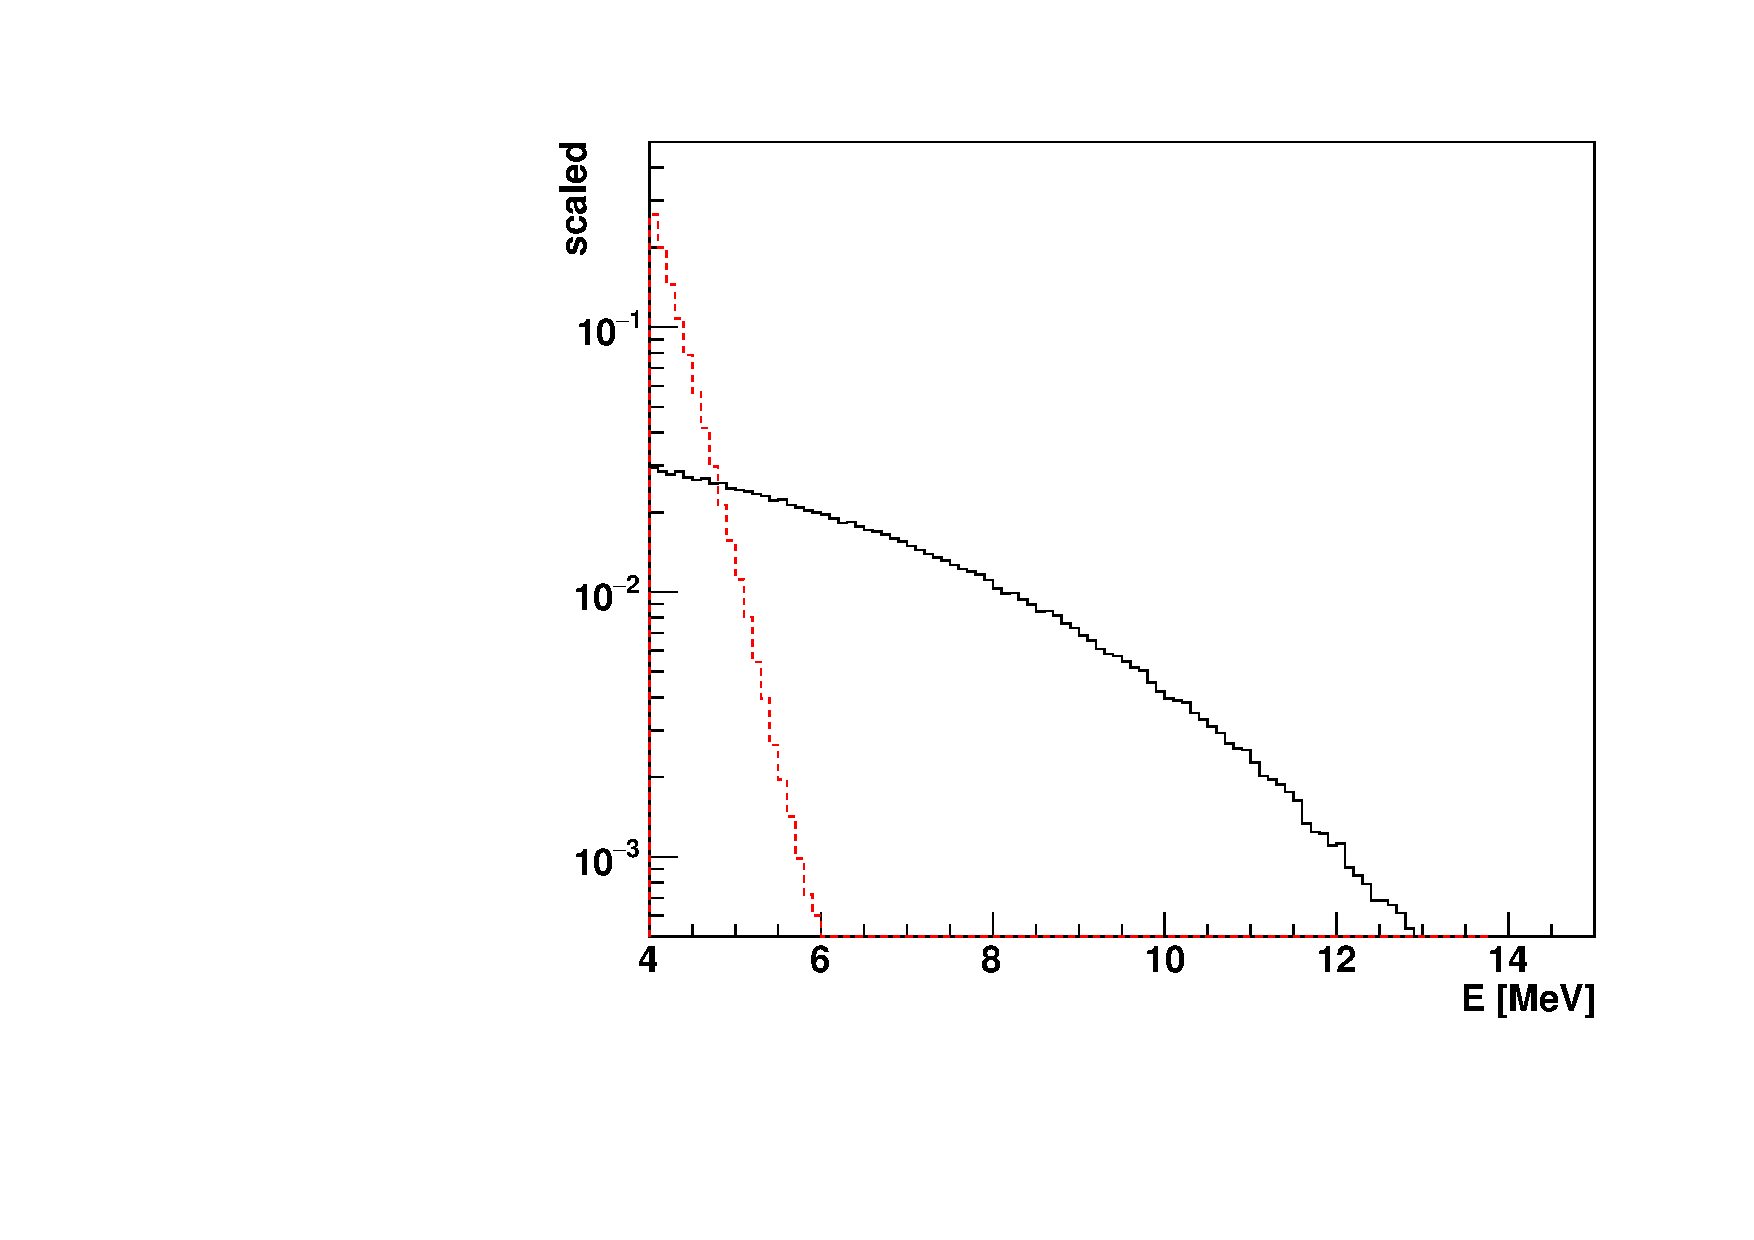
\includegraphics[width=4cm]{tmvaCompare_energy.pdf}
		\end{minipage}
	}
	\subfigure[$G_{test}$]{
		\begin{minipage}[b]{0.3\textwidth}
			\centering
			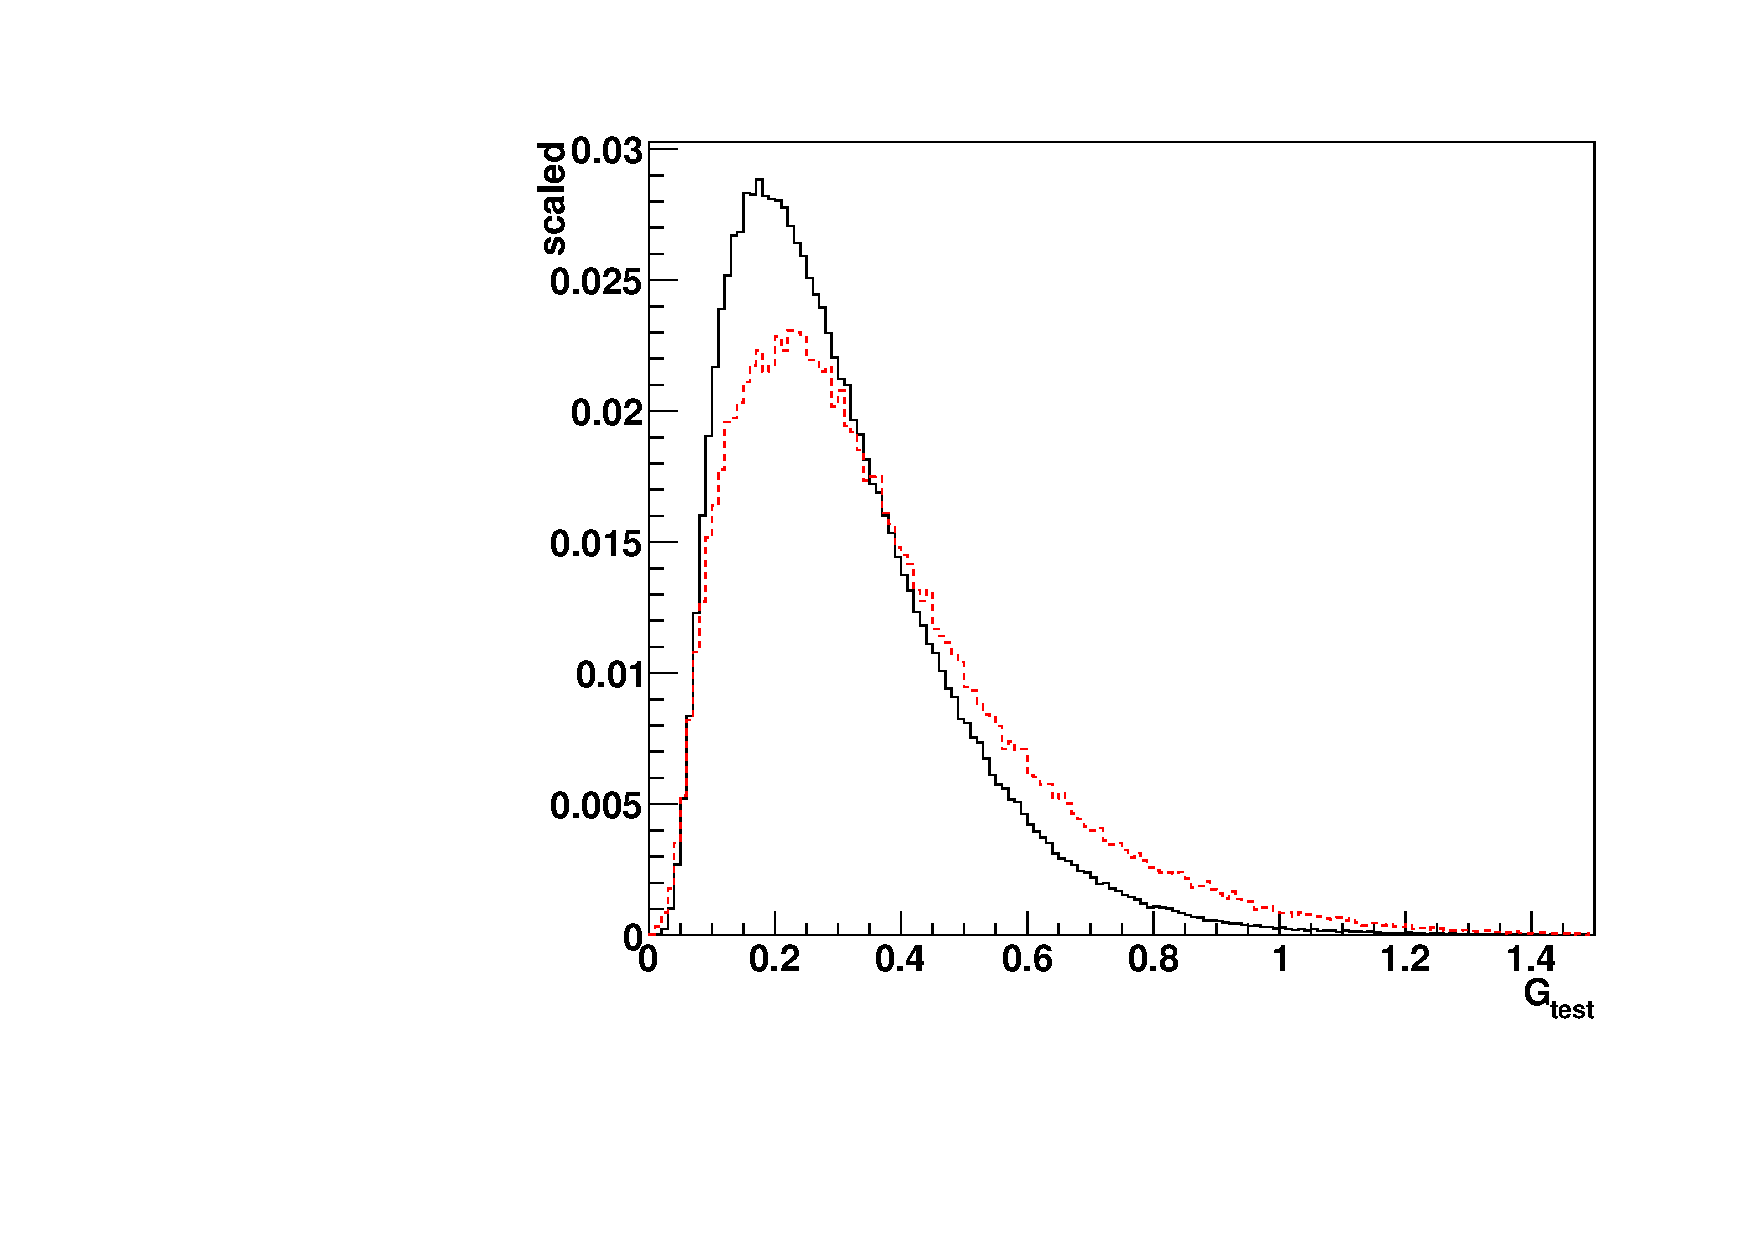
\includegraphics[width=4cm]{tmvaCompare_Gtest.pdf}
		\end{minipage}
	}
	\subfigure[$U_{test}$]{
	\begin{minipage}[b]{0.3\textwidth}
		\centering
		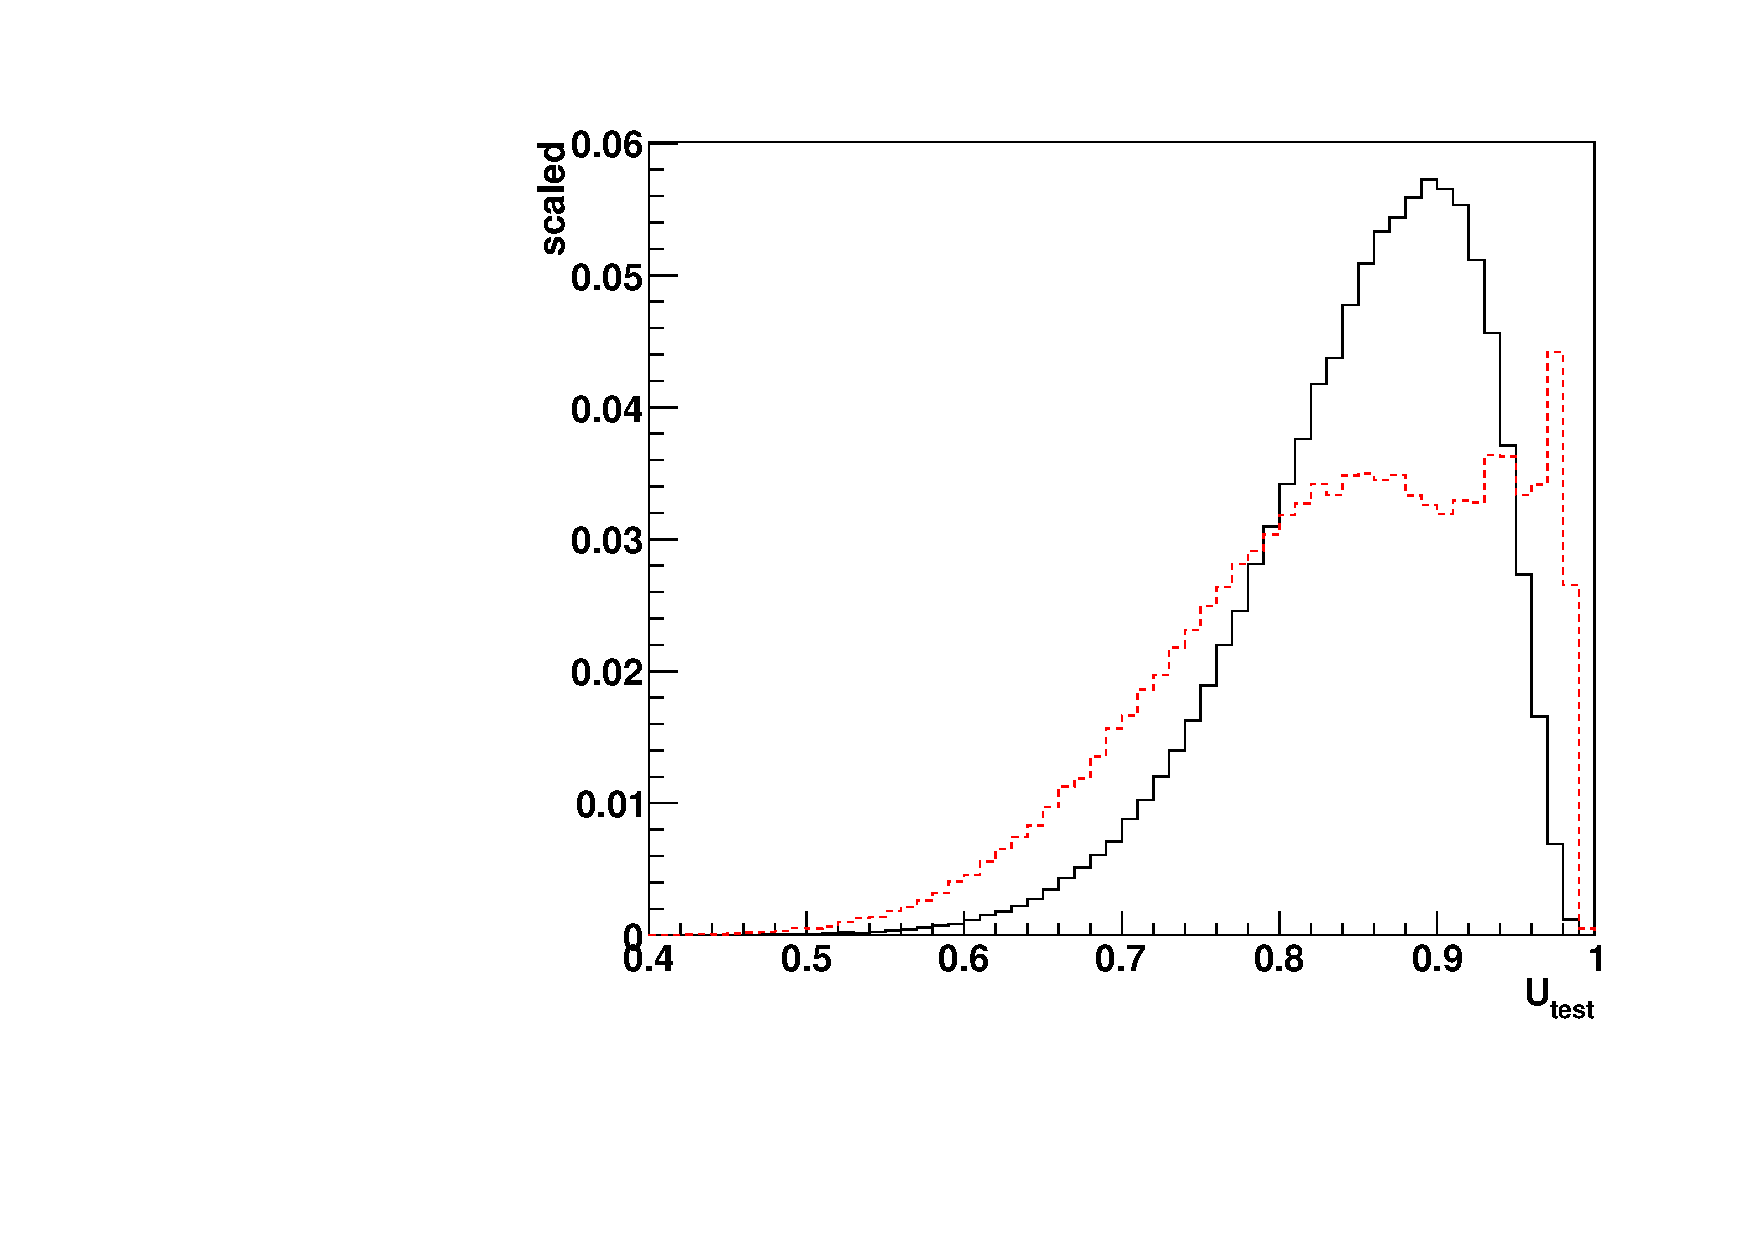
\includegraphics[width=4cm]{tmvaCompare_Utest.pdf}
	\end{minipage}
    }	
   \subfigure[$Z_{factor}$]{
   \begin{minipage}[b]{0.3\textwidth}
	\centering
	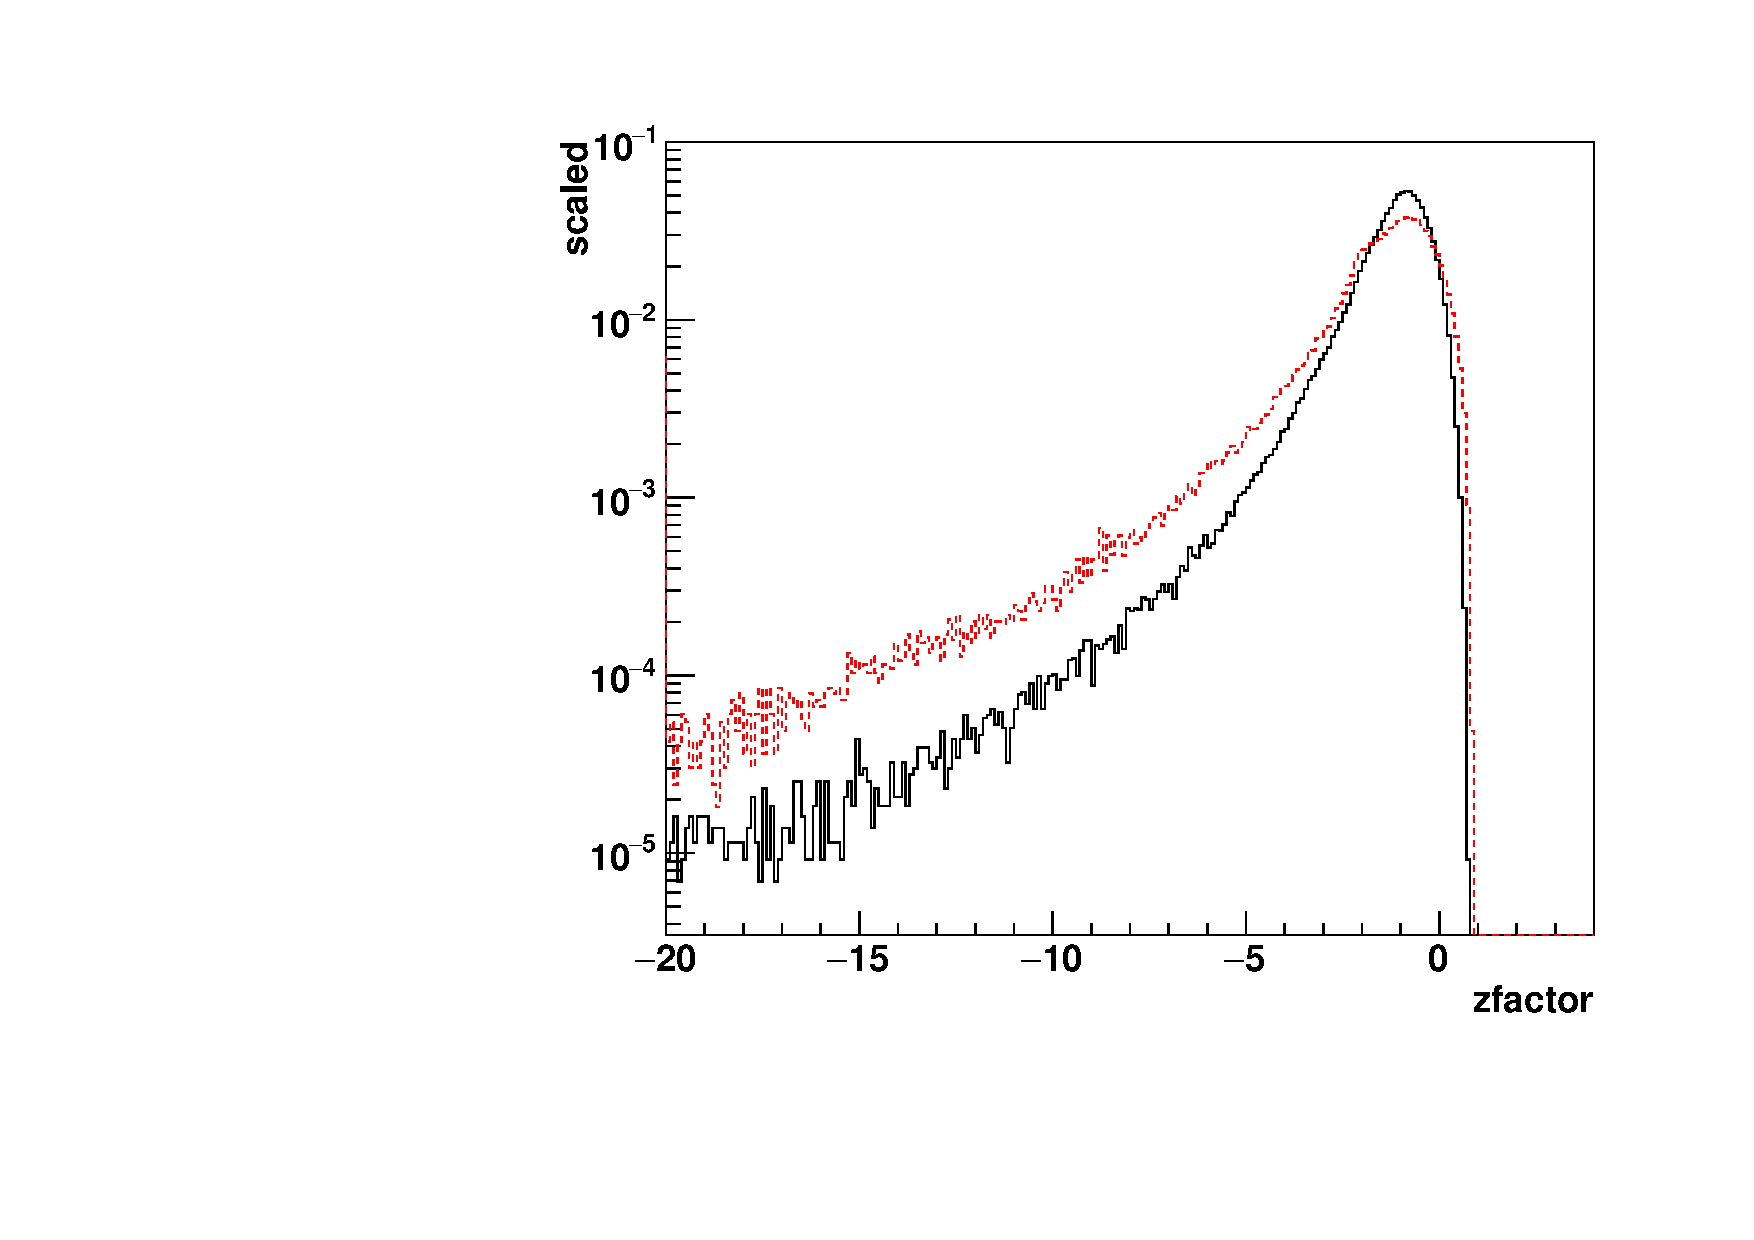
\includegraphics[width=4cm]{tmvaCompare_zfactor.pdf}
   \end{minipage}
   }	
   \subfigure[$ITR$]{
   \begin{minipage}[b]{0.3\textwidth}
	\centering
	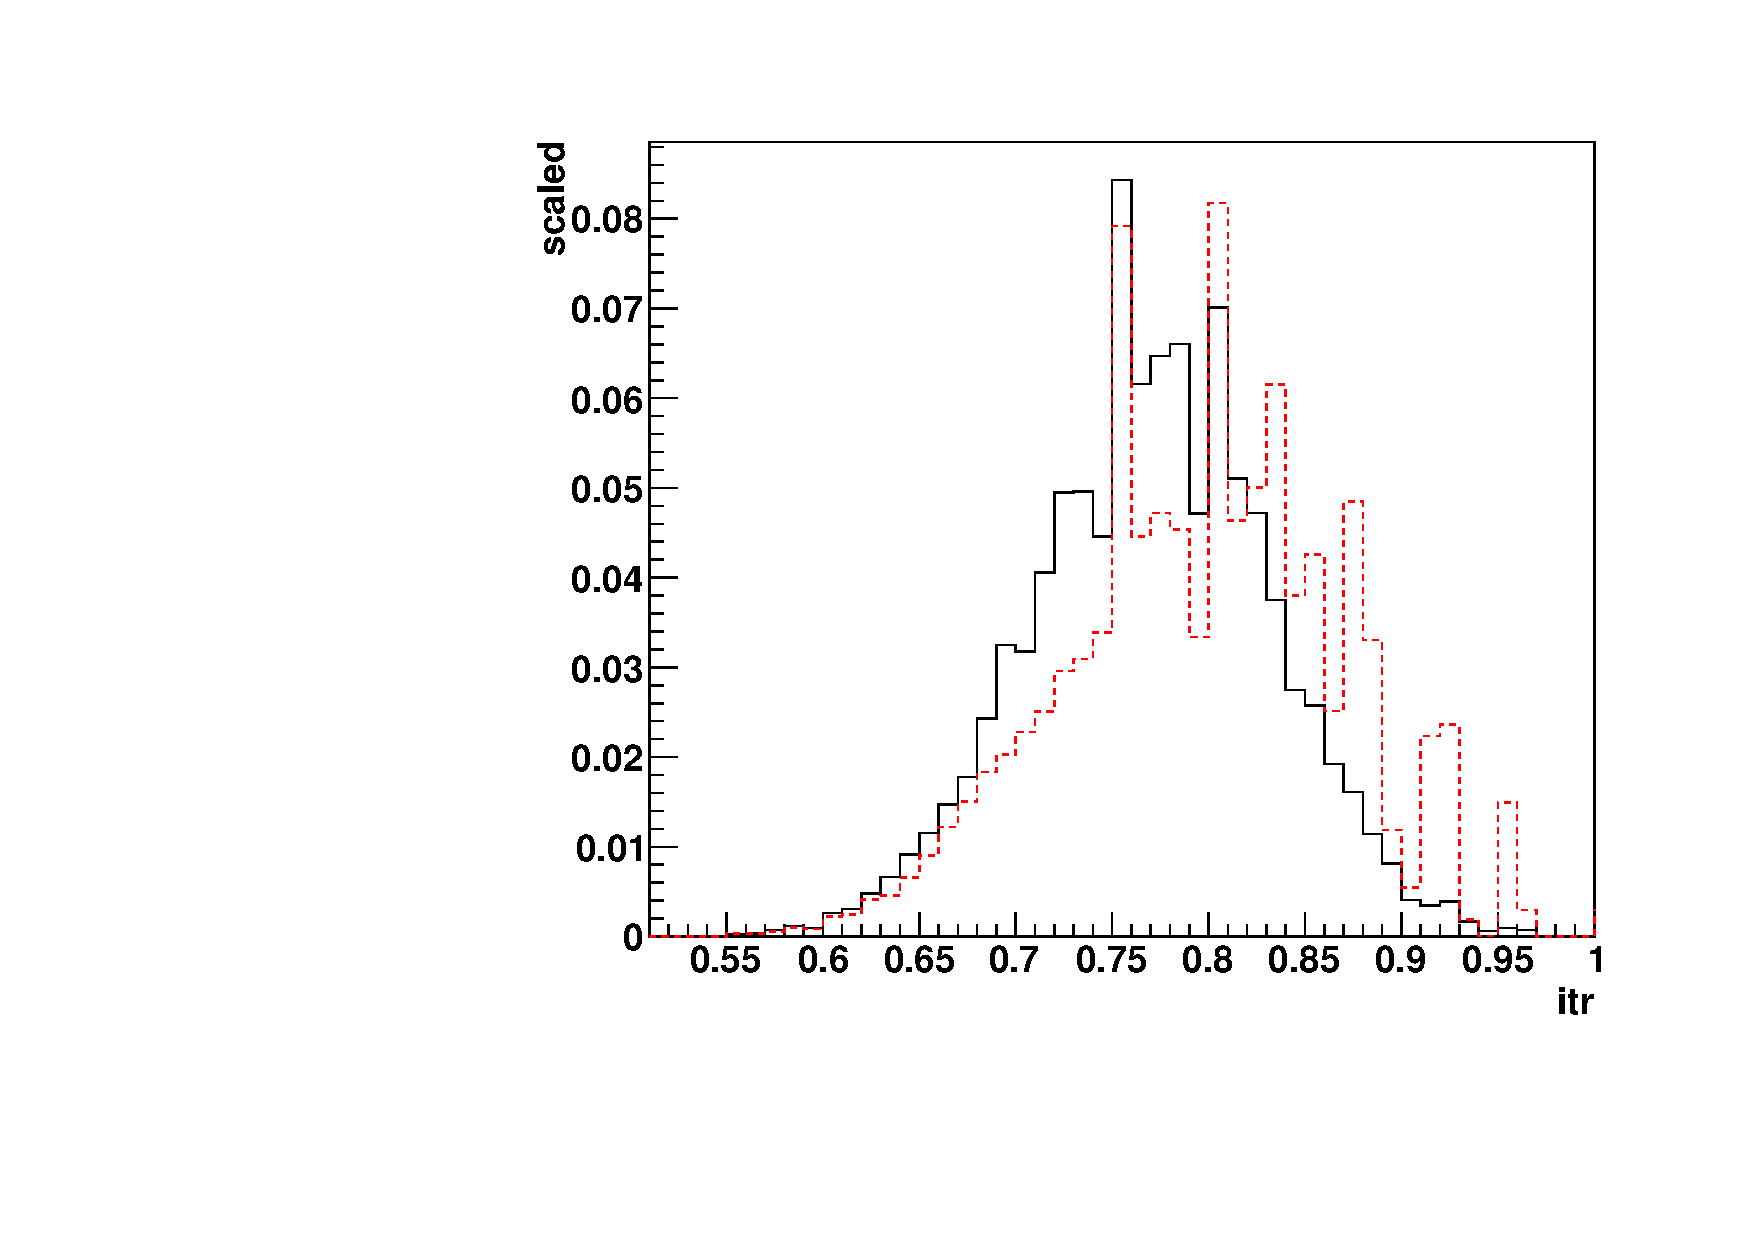
\includegraphics[width=4cm]{tmvaCompare_itr.pdf}
    \end{minipage}
   }	
   \subfigure[$\vec{u}\cdot\vec{R'}$]{
   \begin{minipage}[b]{0.3\textwidth}
	\centering
	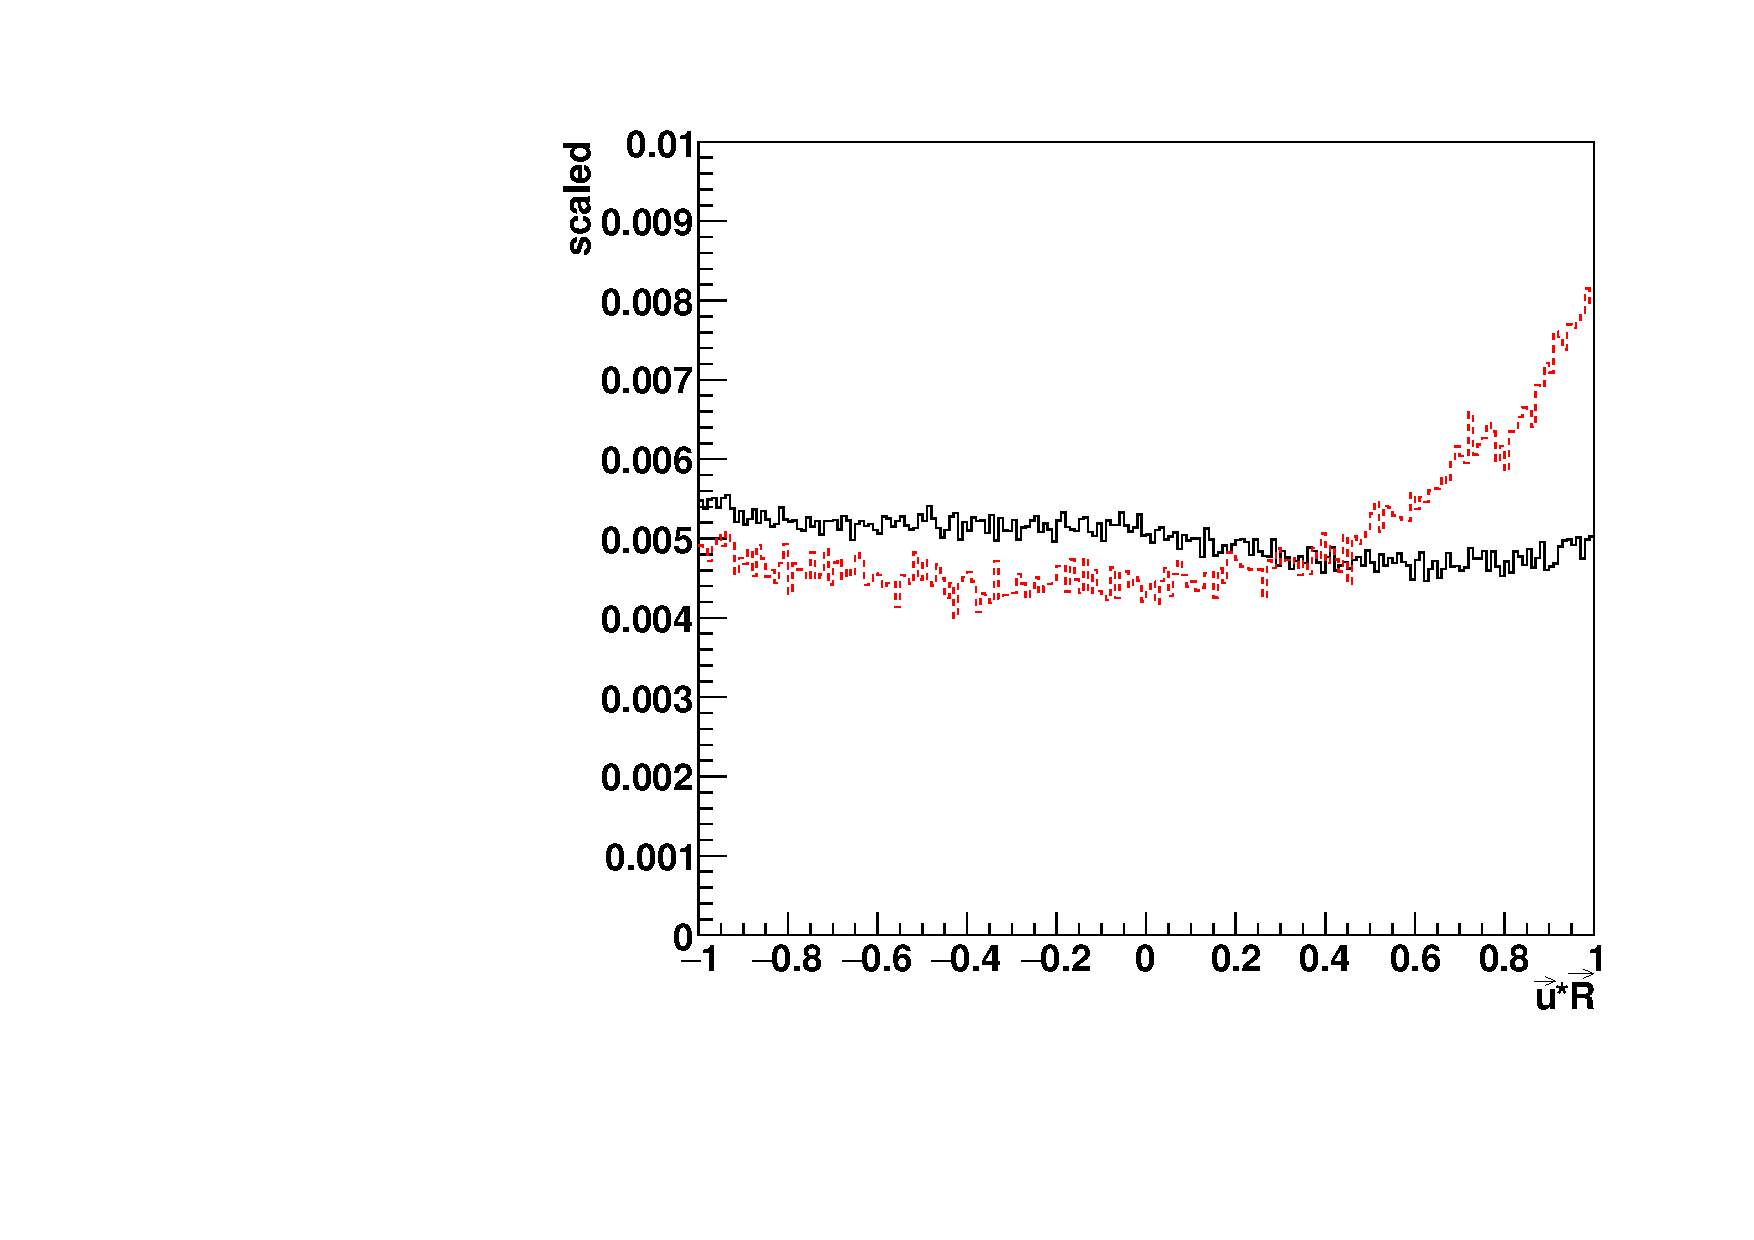
\includegraphics[width=4cm]{tmvaCompare_udotR.pdf}
    \end{minipage}
}
   \subfigure[$scaleLogL$]{
	\begin{minipage}[b]{0.3\textwidth}
		\centering
		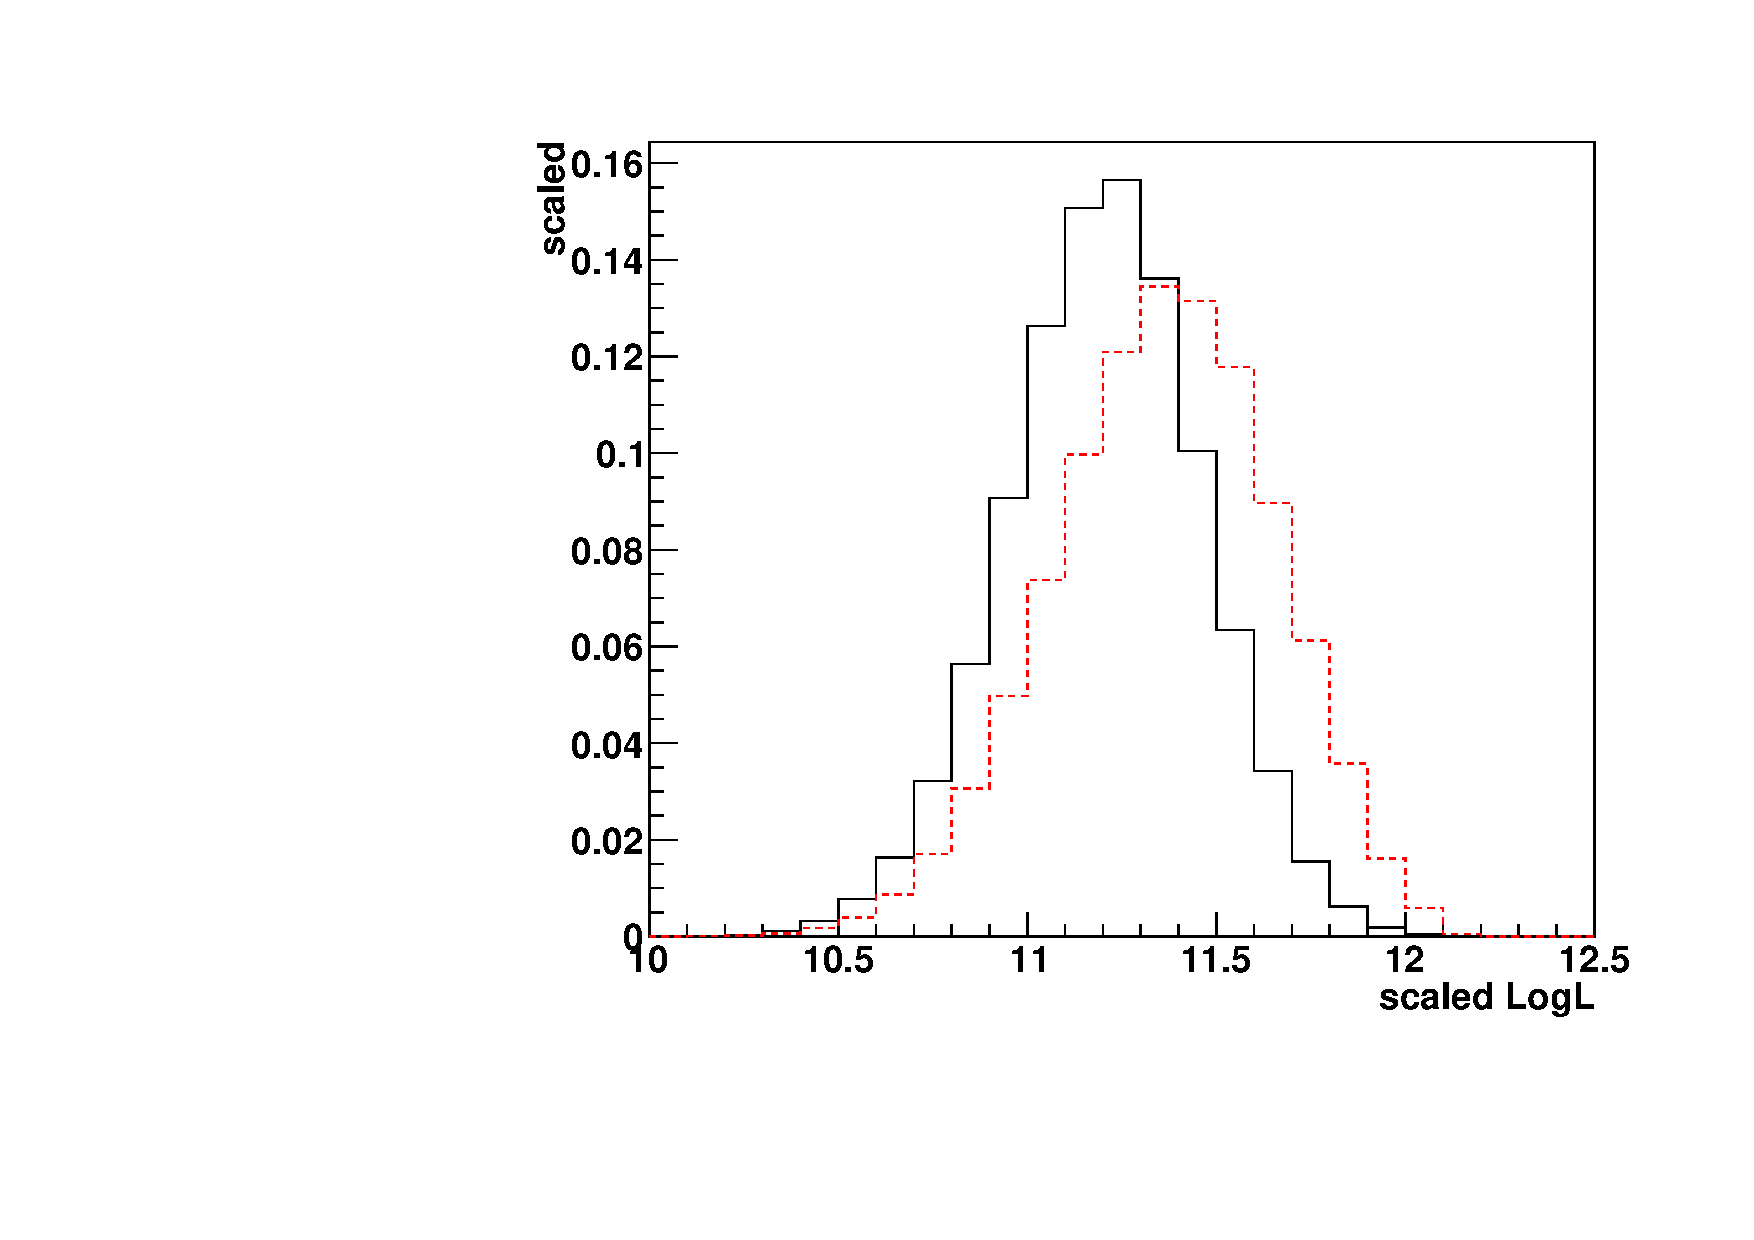
\includegraphics[width=4cm]{tmvaCompare_scaleLogL.pdf}
	\end{minipage}
}	
   \subfigure[$klDiv$]{
    \begin{minipage}[b]{0.3\textwidth}
	\centering
	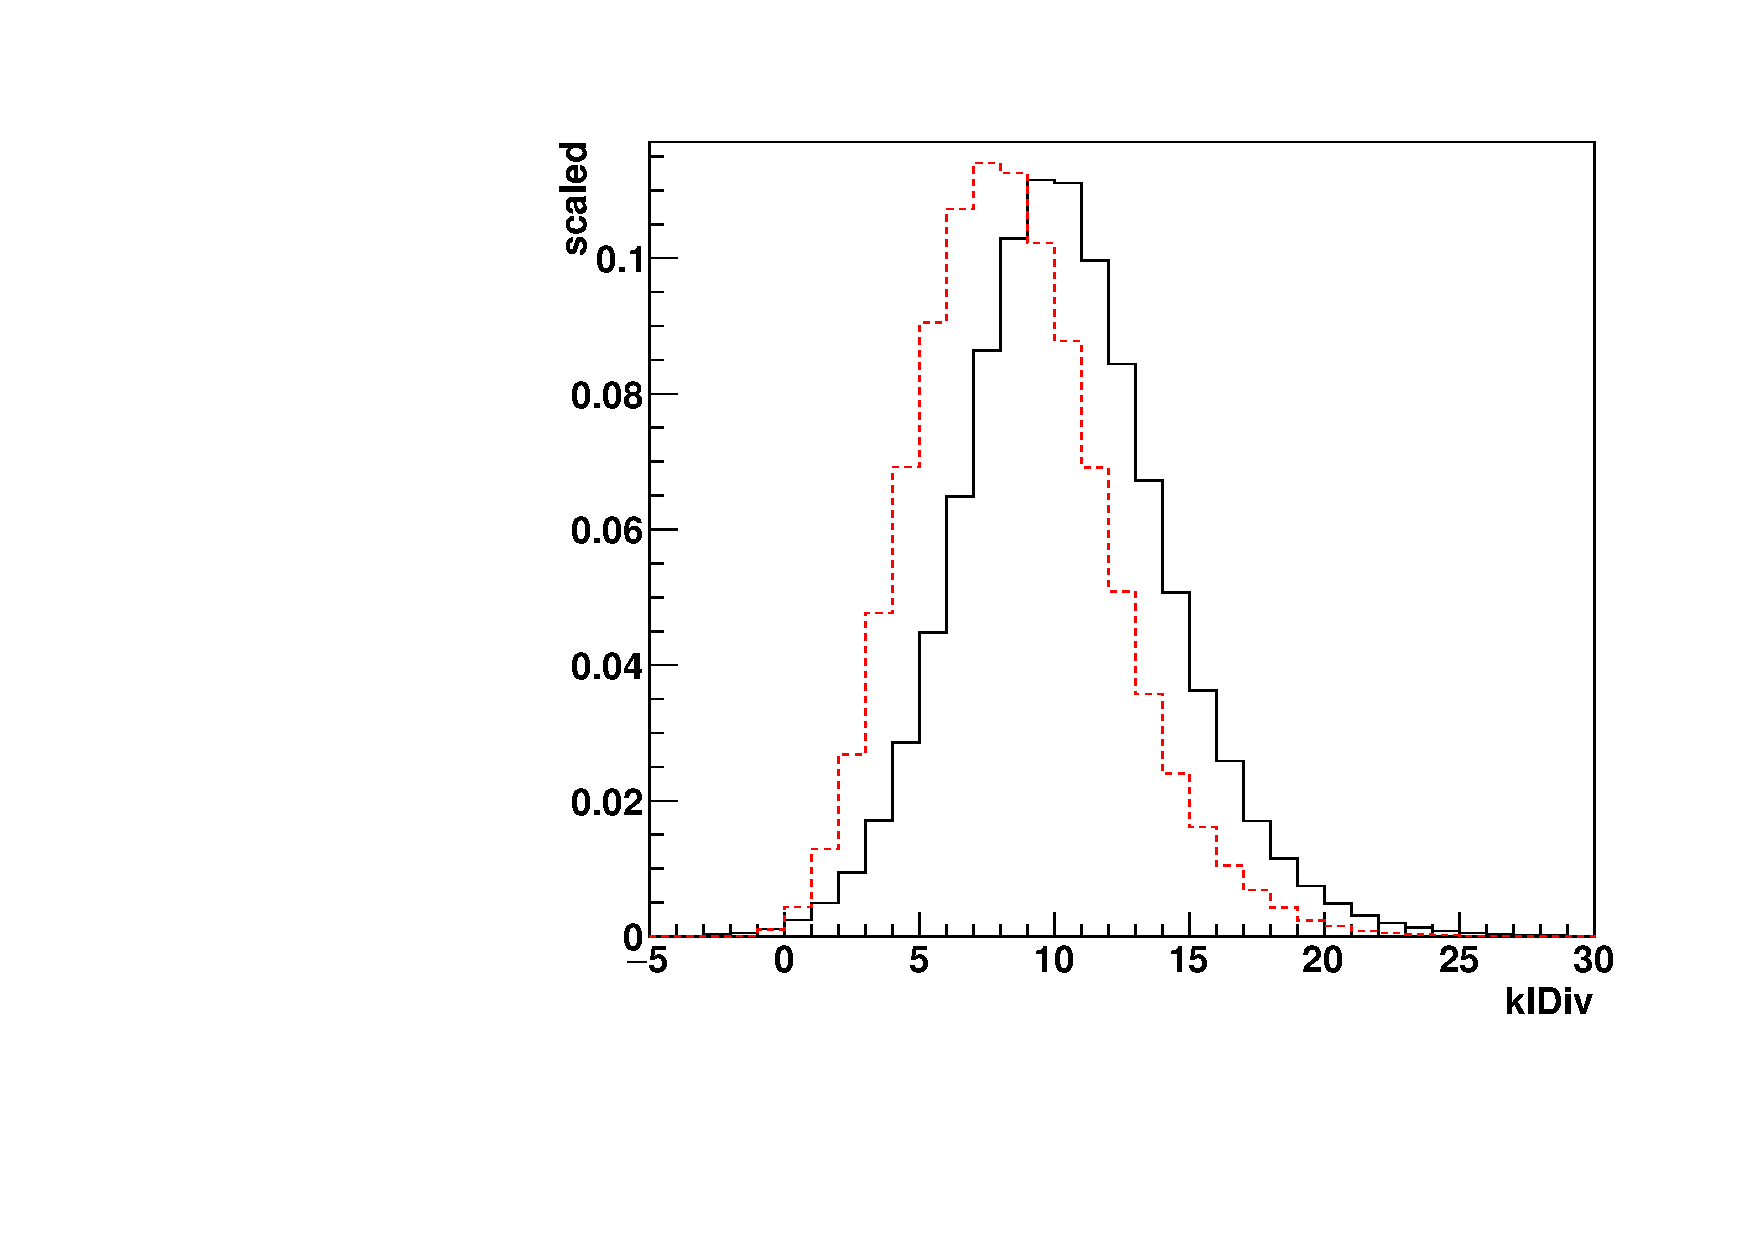
\includegraphics[width=4cm]{tmvaCompare_klDiv.pdf}
   \end{minipage}
   }
%   \subfigure[$\cos\theta_{sun}$]{
%	\begin{minipage}[b]{0.3\textwidth}
%		\centering
%		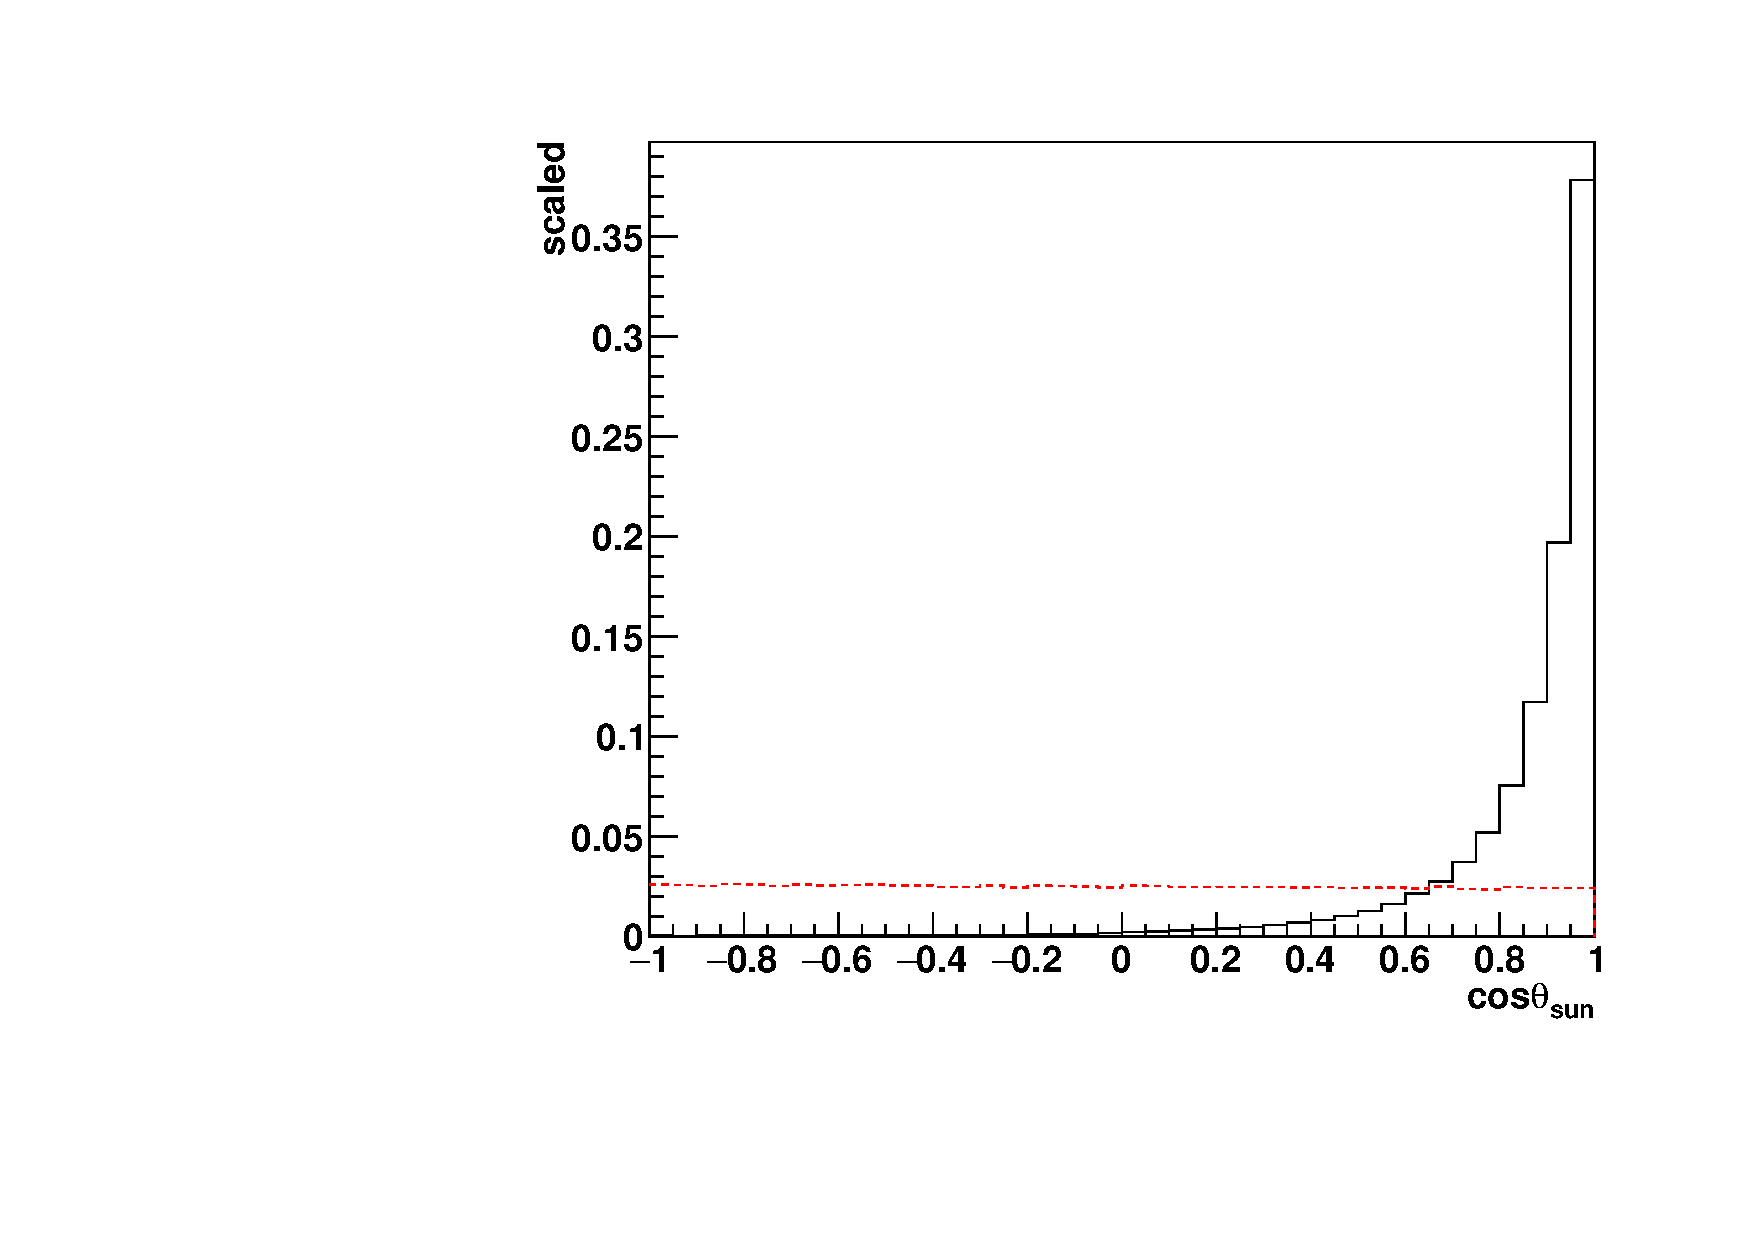
\includegraphics[width=4cm]{tmvaCompare_cosThetaSun.pdf}
%	\end{minipage}
%   }	
	\caption[Multiple variables as the inputs for the TMVA analysis.]{Multiple variables as the inputs for the TMVA analysis. The distributions of the backgrounds are show in dotted red lines while the signals are shown in solid black lines. The distributions are normalized to their integrals.\label{fig:inputParamsTMVA}}
\end{figure}

The MLP method gave the best results, while it was the most CPU-consuming method.

The output signal/background distributions on the test sub-dataset are shown in Fig.~\ref{output_separation_allE}.
\begin{figure}[htbp]
	\centering
	\subfigure[Fisher/LD output.]{
		\begin{minipage}[t]{0.4\textwidth}
			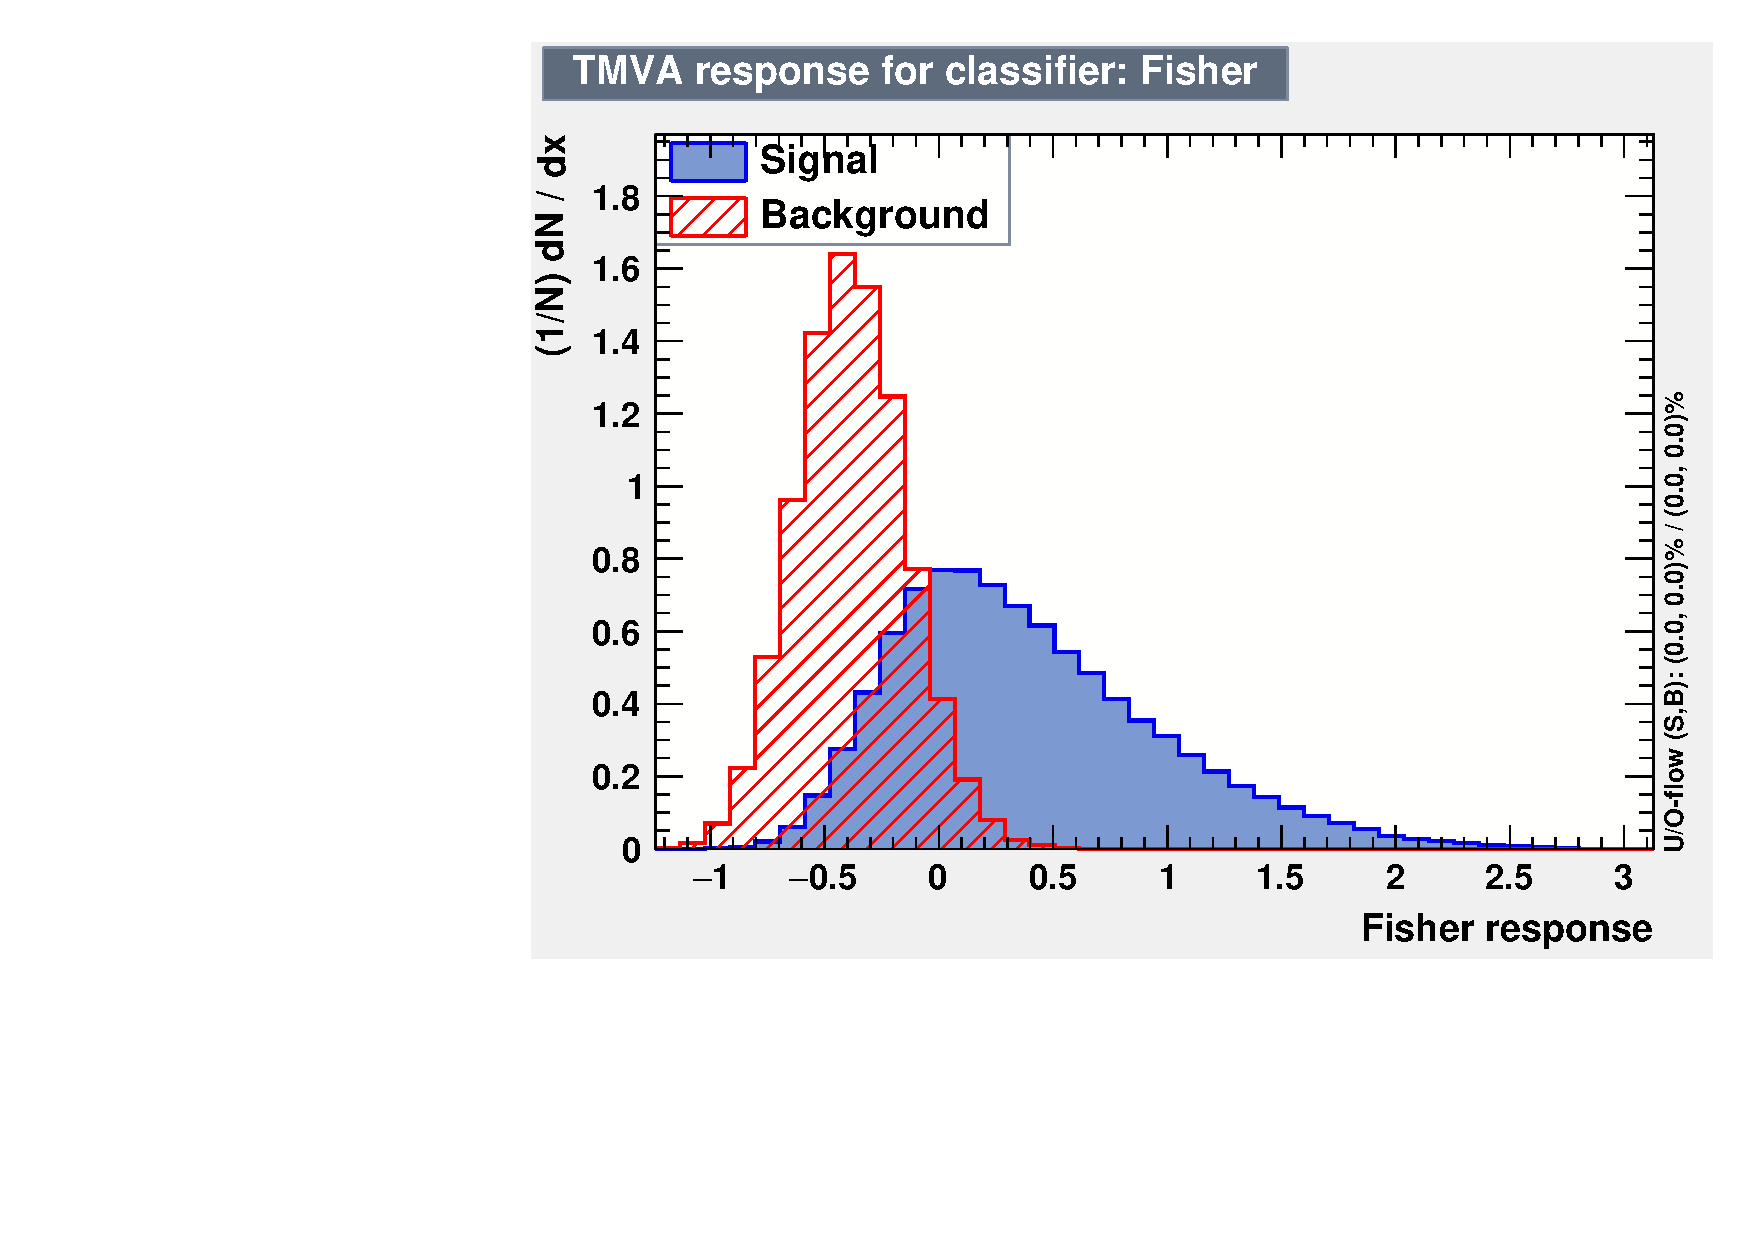
\includegraphics[width=6cm]{output_allE_Fisher.pdf}
		\end{minipage}
	}
	\subfigure[BDT output.]{
		\begin{minipage}[b]{0.4\textwidth}
			\centering
			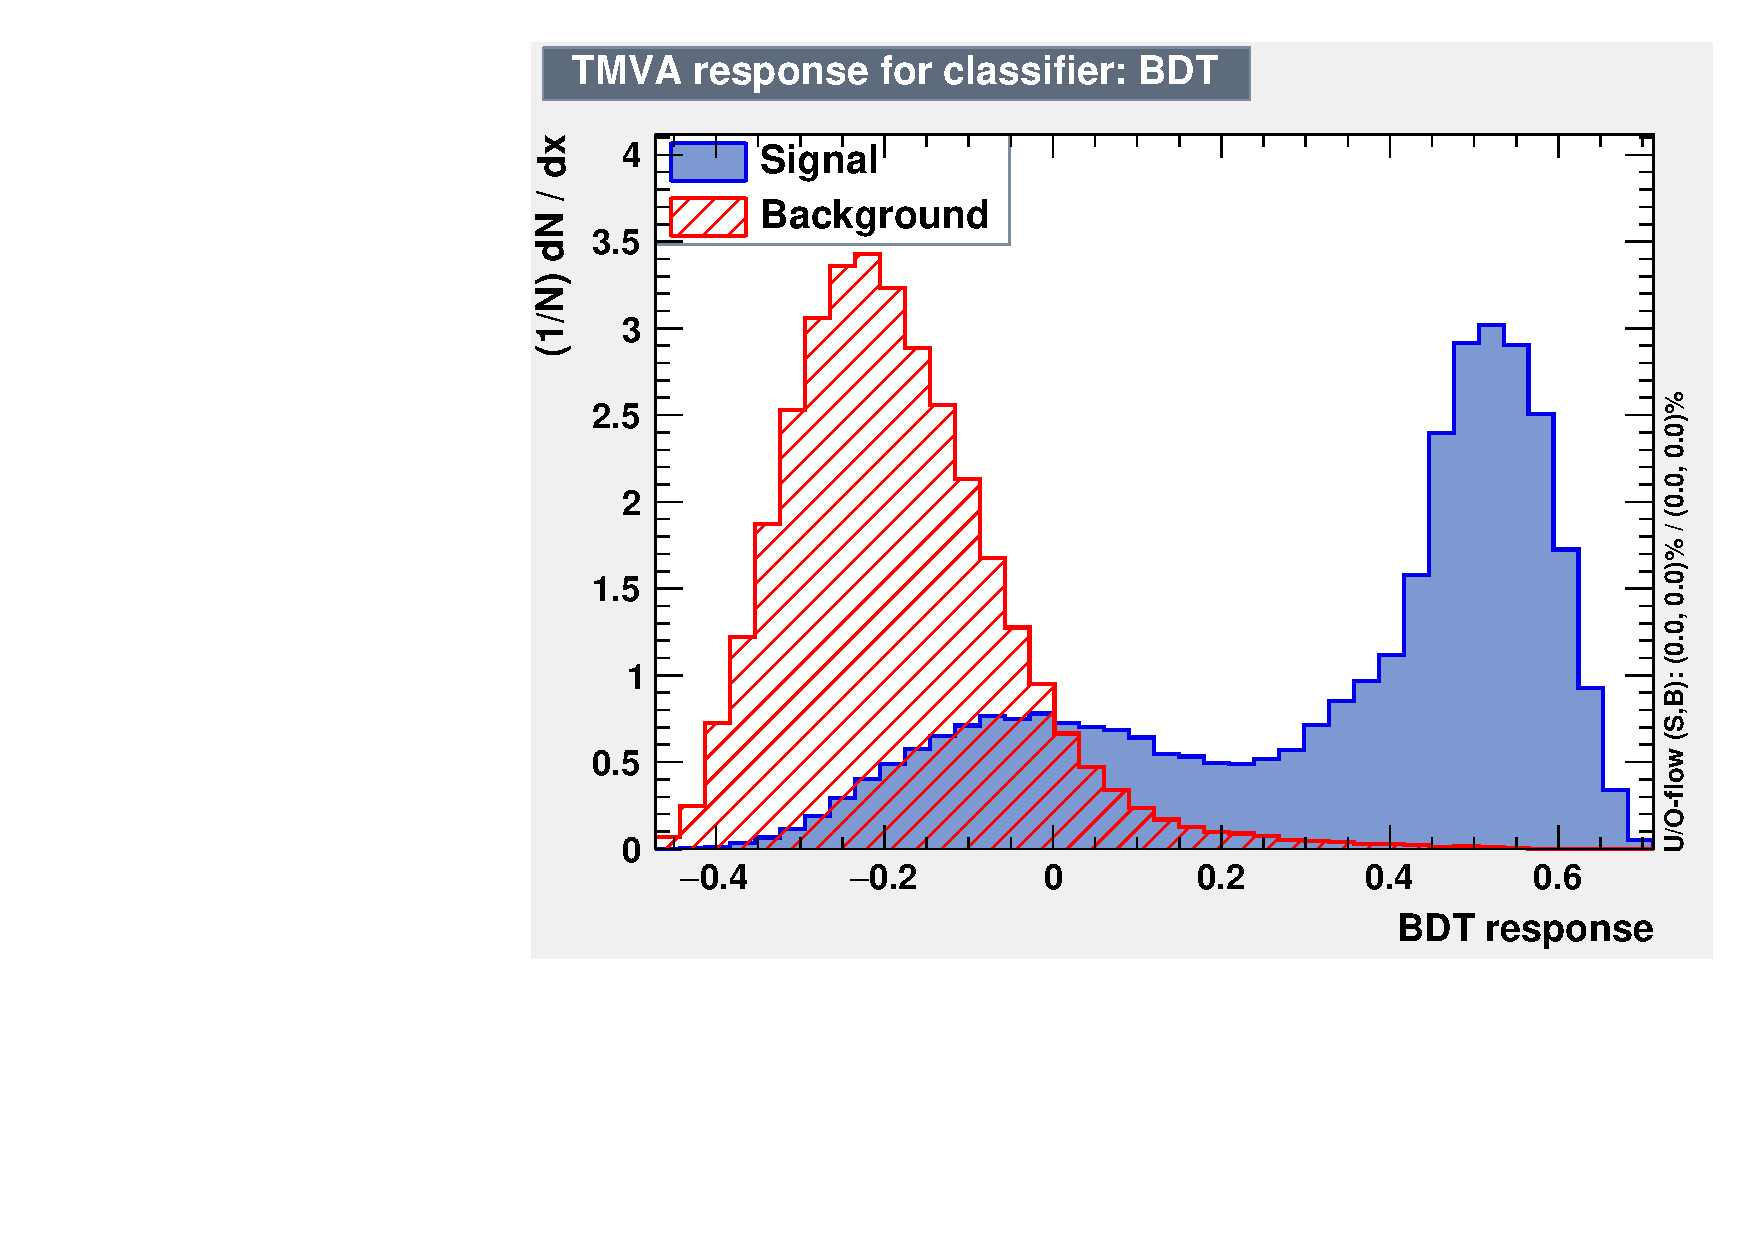
\includegraphics[width=6cm]{output_allE_BDT.pdf}
		\end{minipage}
	}
	\subfigure[MLP output]{
		\begin{minipage}[b]{0.4\textwidth}
			\centering
			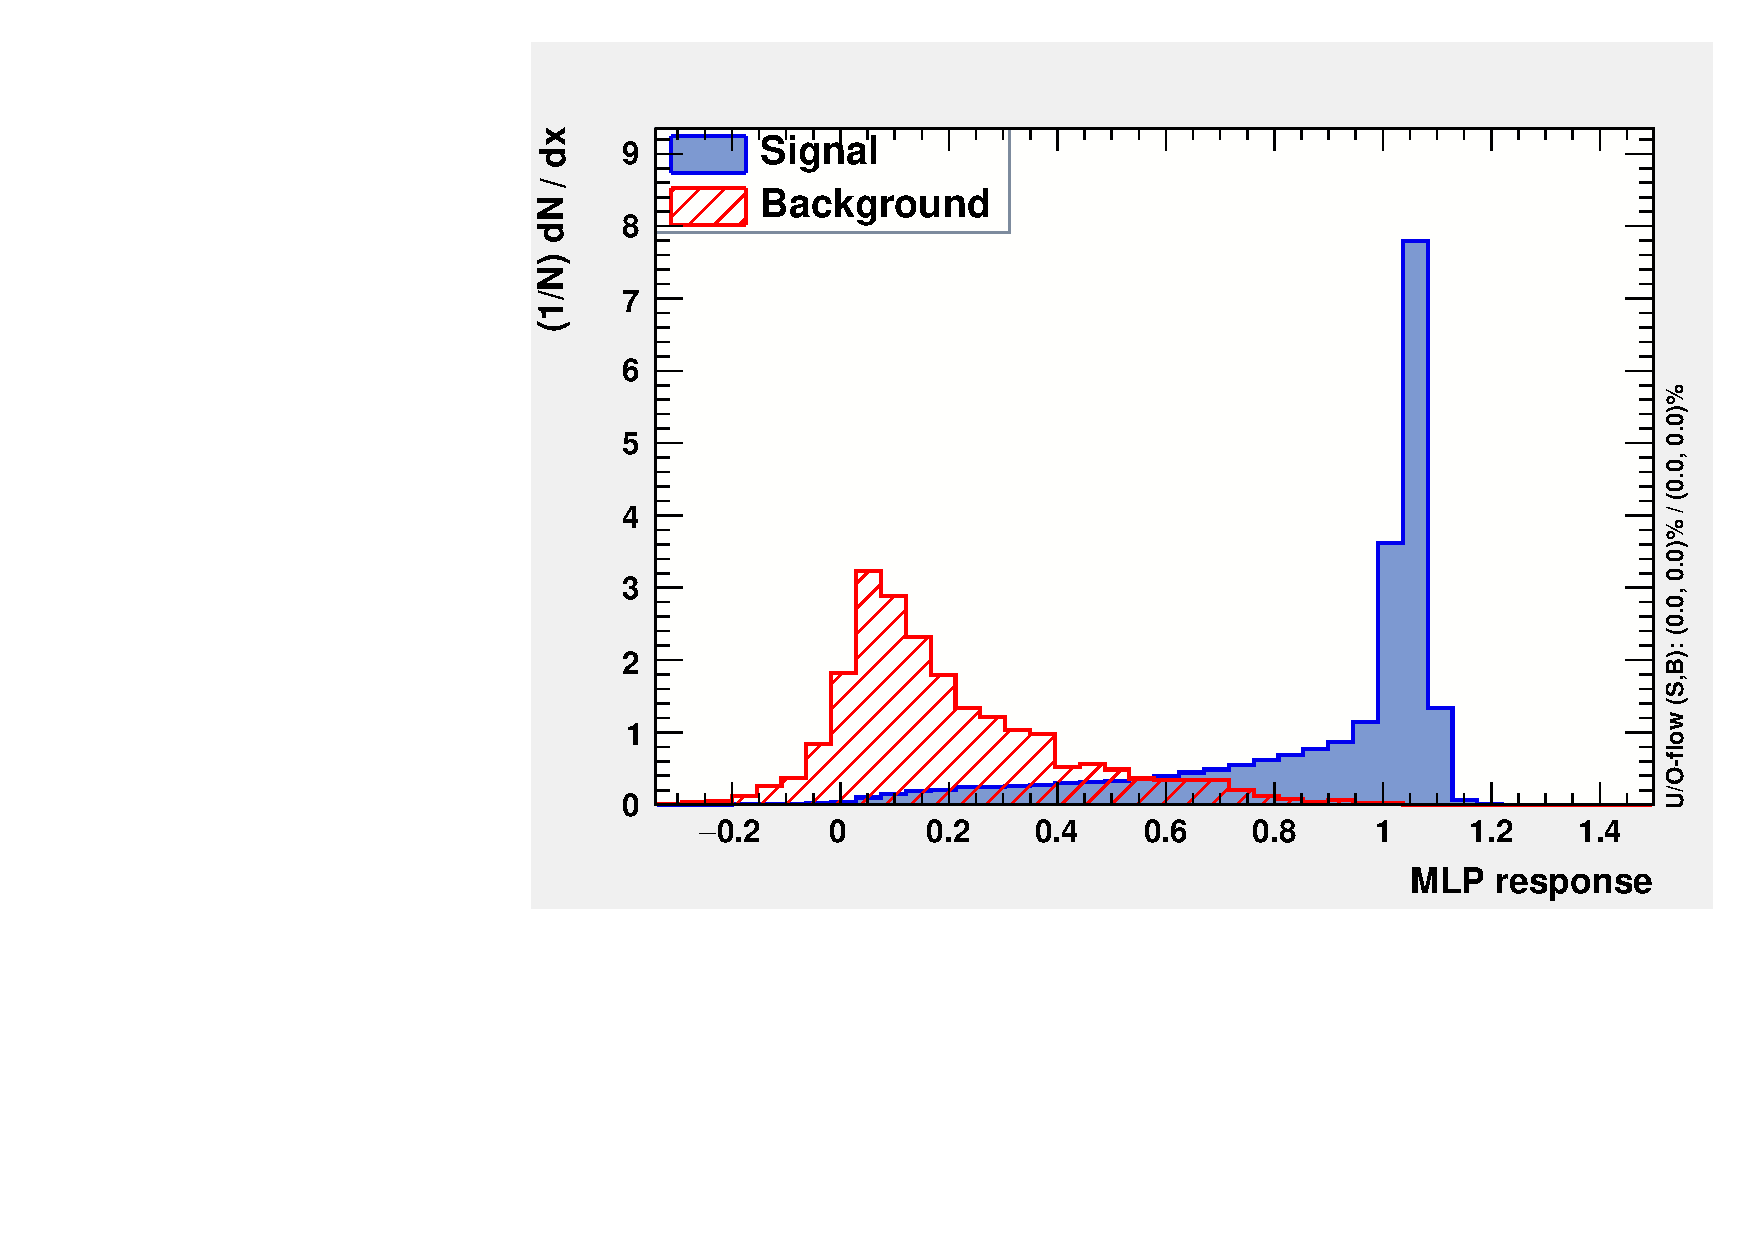
\includegraphics[width=6cm]{output_allE_MLP.pdf}
		\end{minipage}
	}
	\caption{TMVA outputs for signal/background separations by different methods.\label{output_separation_allE}}
\end{figure}

As one of the essential TMVA output, the background rejection versus signal efficiency curve is denoted as a receiver operating characteristic (ROC) curve, which is usually used to test the performance of machine learning classifier. A quantity taking the integrals of the ROC curve: called the ``area under the curve'' (AUC) is often used to summarize the quality of a ROC curve\cite{murphy2012machine}.  Fig.~\ref{allE_roc} shows the ROC curves for different methods:
\begin{figure}[!htb]
	\centering
	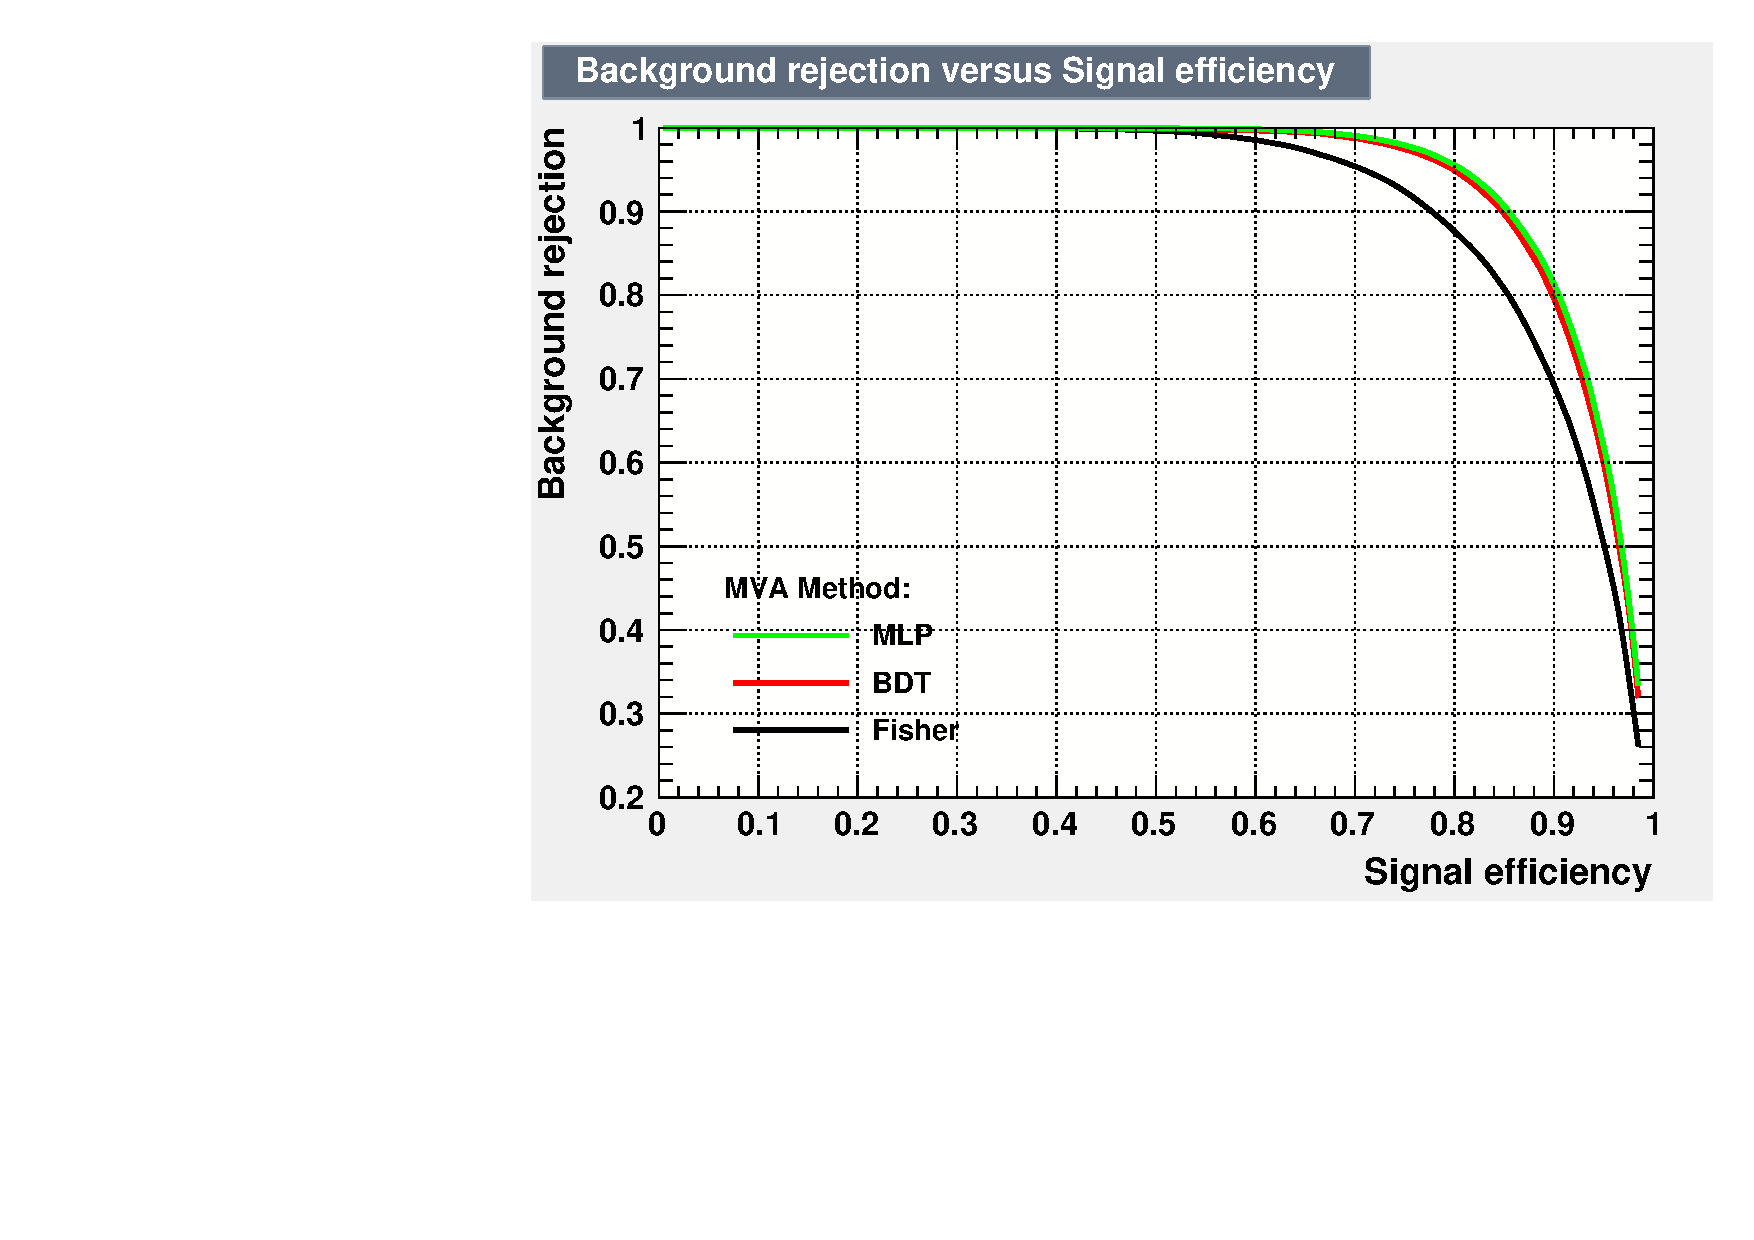
\includegraphics[width=10cm]{ROC_E4to15.pdf}
	\caption{ROC curves from TMVA output, for event with $4<E_{fit}<15$~MeV.}
	\label{allE_roc}
\end{figure}
where the Fisher/LD is the worst case; the BDT and MLP outputs are close to each other while the MLP gives the largest AUC values.

\begin{figure}[!htb]
	\centering
	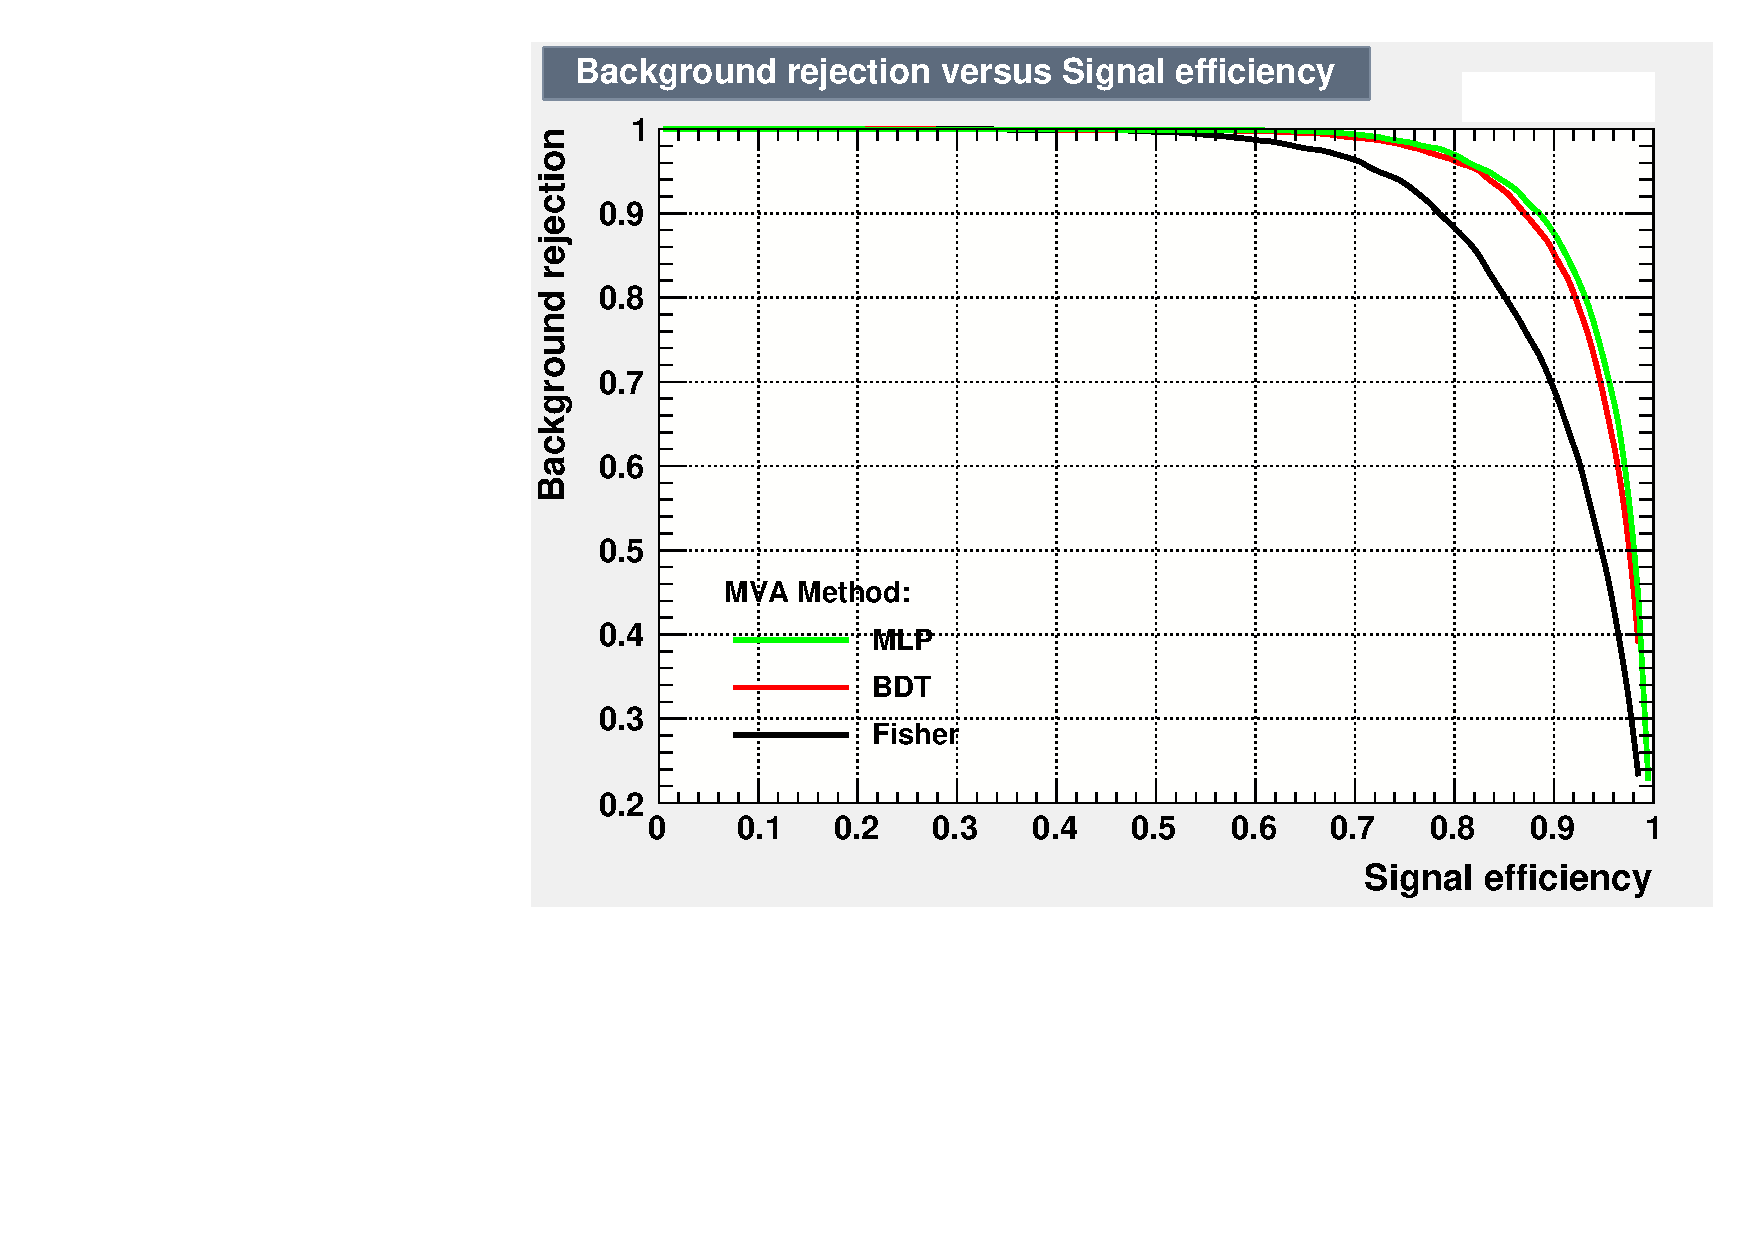
\includegraphics[width=10cm]{ROC_E5to15.pdf}
	\caption{ROC curves from TMVA output, for event with $5<E_{fit}<15$ MeV (energy above 5 MeV).}
	\label{E5to15_roc}
\end{figure}

\begin{figure}[!htb]
	\centering
	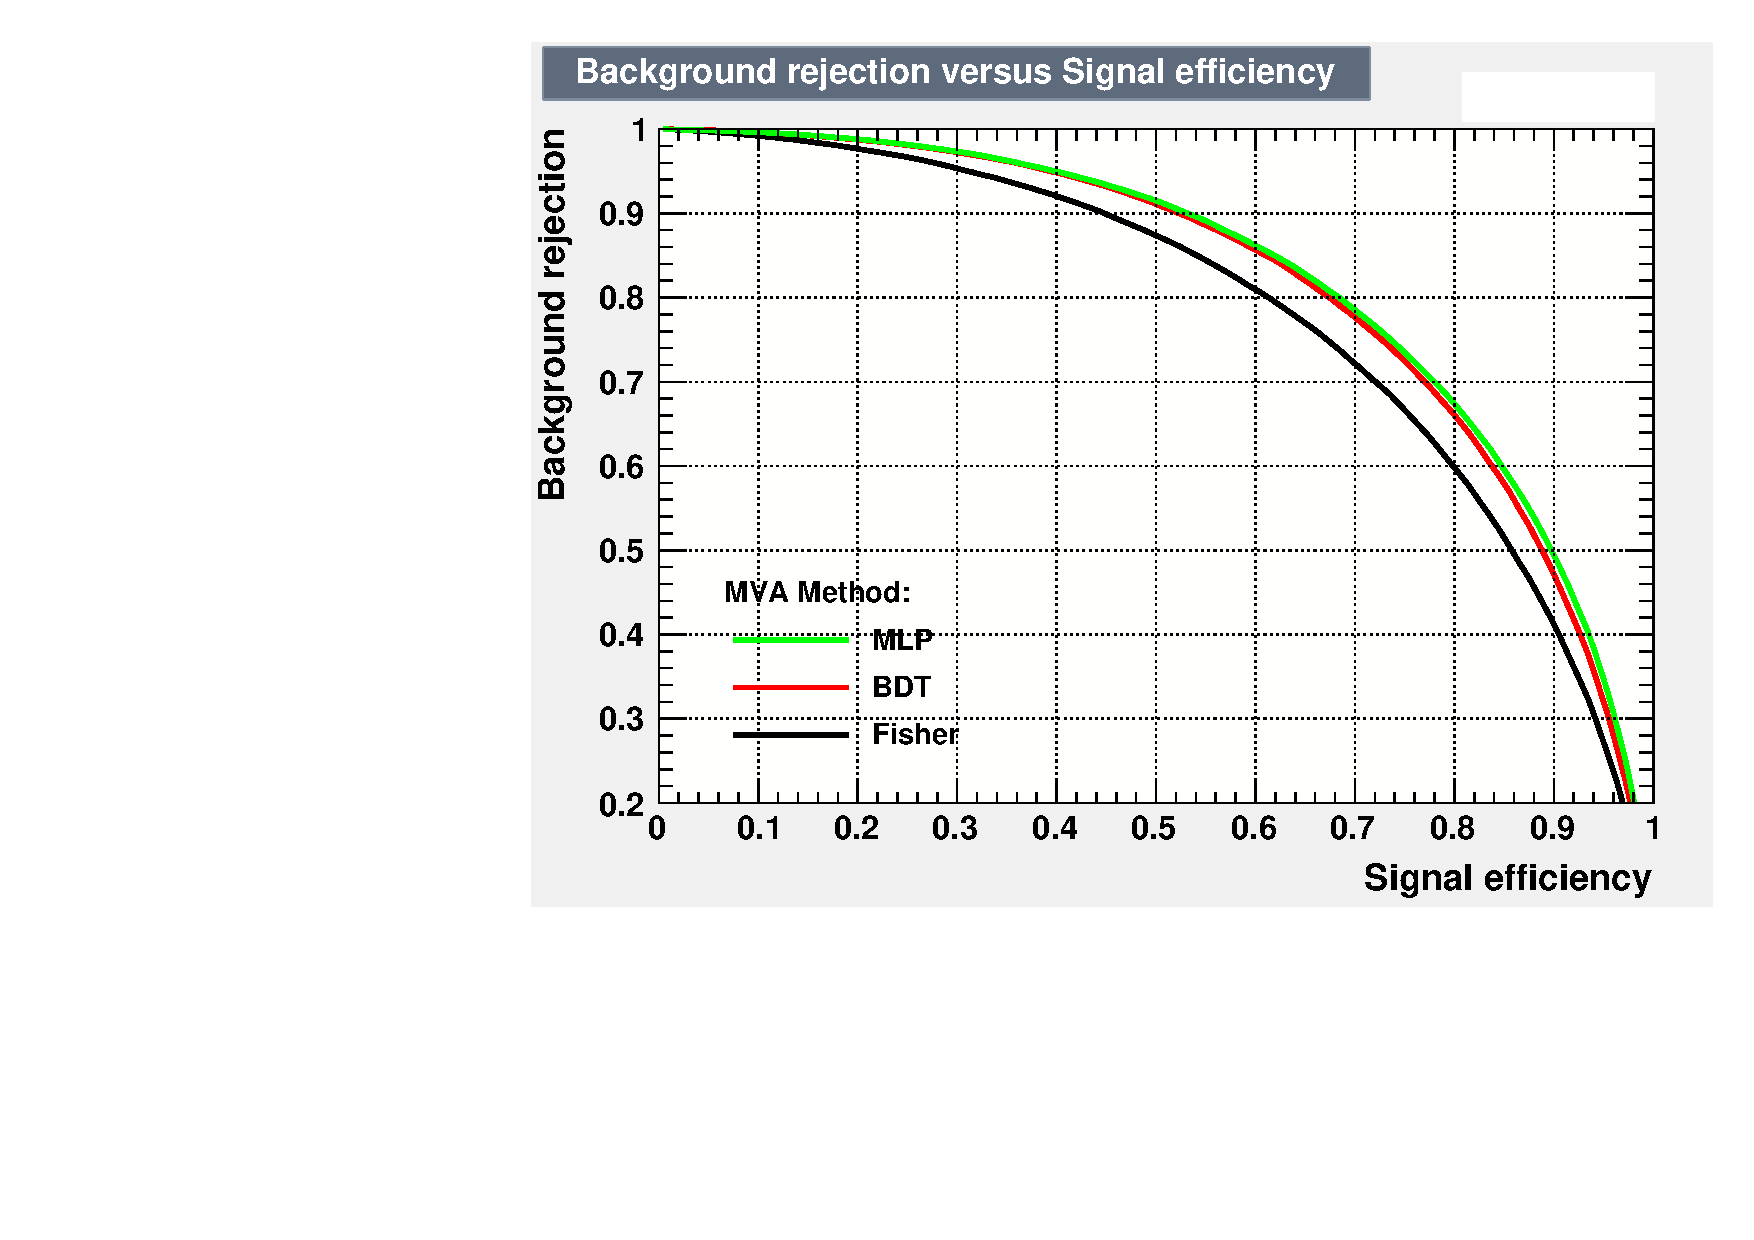
\includegraphics[width=10cm]{ROC_E4to5.pdf}
	\caption{ROC curves from TMVA output, for event with $4<E_{fit}<5$ MeV (low energy region).}
	\label{E4to5_roc}
\end{figure}

A typical CPU time ($t_{CPU}$) for a certain method to train the dataset with different energy regions is listed in Table.~\ref{tab:tmvaMethod_allE}.
\begin{table}[ht]
	\centering
	\caption{Testing results from different TMVA methods.}
	\label{tab:tmvaMethod_allE}
	\begin{tabular*}{100mm}{c@{\extracolsep{\fill}}ccc}
		\toprule
		Method & AUC & $t_{CPU}$ (second/$10^6$ events) \\
		\midrule
		$4<E_{fit}<15$~MeV \\
		Fisher/LD & 0.915 & 0.81\\
		BDT &  0.940 & 249.53 \\
		MLP & 0.944 & 1370.02\\
	   \hline
	   $5<E_{fit}<15$ MeV\\
				Fisher/LD & 0.915& 0.93\\
		BDT & 0.950 & 269.71\\
		MLP &  0.958 & 1450.90\\
	   \hline
	   $4<E_{fit}<5$ MeV \\
	   Fisher/LD & 0.782 & 0.84\\
		BDT & 0.816 & 280.1\\
		MLP & 0.823 &1337.9\\
		\bottomrule
	\end{tabular*}
\end{table}

It shows that, when the energy goes lower, it is more difficult to separate the signals from the backgrounds.

The distributions of the ``solar angle'', $\cos\theta_{sun}$ were used to show the performance of the solar $\nu_e$ event selection and background event discrimination. It is also used to extract the number of signal and background events, which will be discussed in the following sections. Here I applied the BDT and the MPL method on the test sub-dataset. For the real dataset from run-200004 to 207718, the trained weights and variables from the BDT and the MLP methods were applied event by event and the discriminator responses, $D_{BDT}$ and $D_{MLP}$ were calculated respectively. Cuts of $D_{BDT}>0.0$ and $D_{MLP}>0.5$ were applied to extract the solar $\nu_e$ signals from backgrounds. 
%The distributions of $\cos\theta_{sun}$ were shown in Fig. as the results.
%4<E<15 MeV
%%BDT signal efficiency     = 0.944954
%% MLP signal efficiency        = 0.926606
 
%MLP signal efficiency        = 0.842493
%MLP background efficiency    = 0.0840084
%5<E<15 MeV
%BDT signal efficiency     = 0.868345w
%BDT background efficiency = 0.103896
%MLP signal efficiency        = 0.887622
%MLP background efficiency    = 0.104416

%%% BDT signal efficiency     = 0.733945
%% MLP signal efficiency        = 0.779817
%
%4<E<5 MeV
%BDT signal efficiency     = 0.72266
%BDT background efficiency = 0.245453
%MLP signal efficiency        = 0.723576
%MLP background efficiency    = 0.235984

%\begin{figure}[!htb]
%	\centering
%	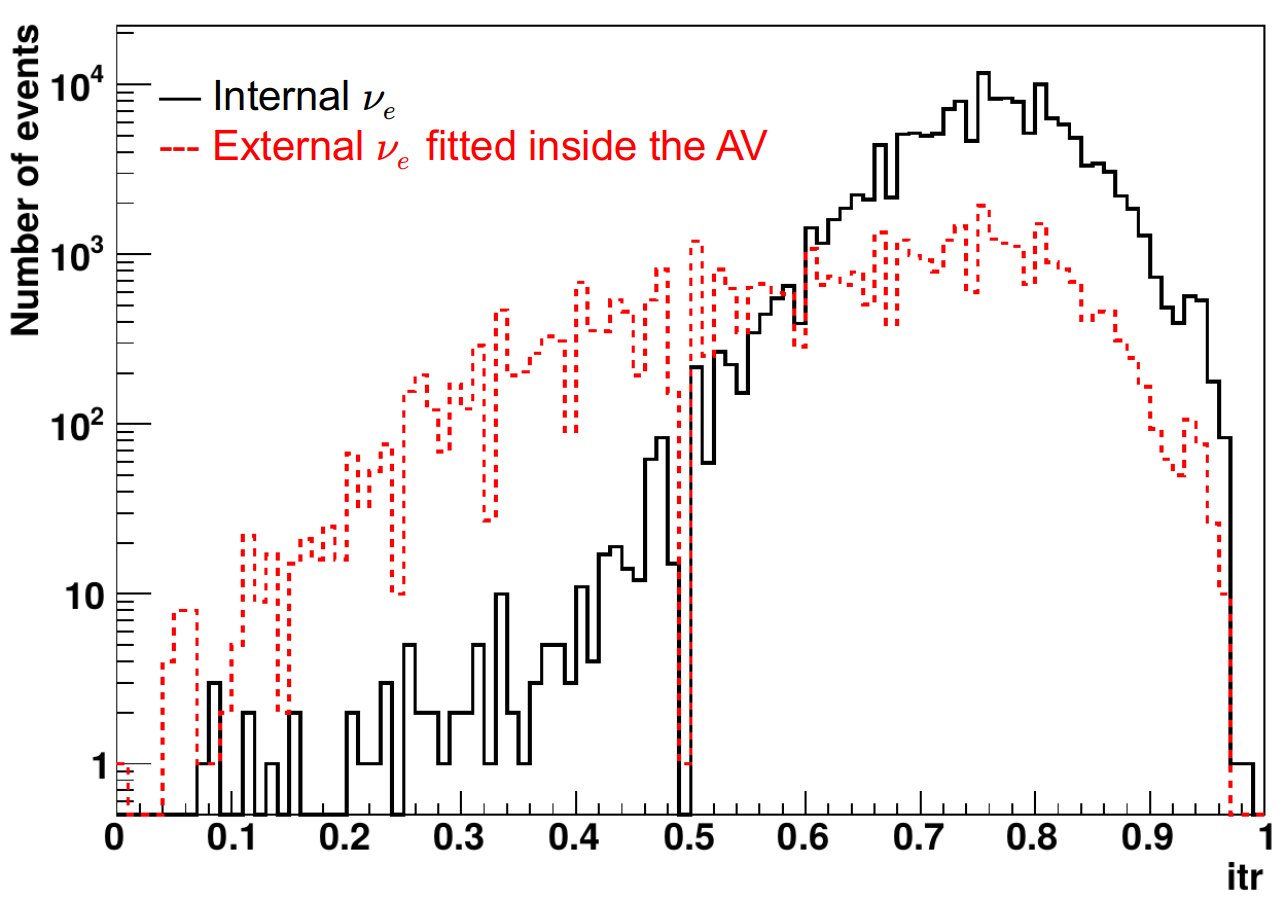
\includegraphics[width=8cm]{ITR_MPW_solarNuVsExSolar.png}
%	\caption{Comparison between solar $\nu_e$ and external solar $\nu_e$; MPW results.}
%	\label{itrCmp}
%\end{figure}
\subsubsection{TMVA Outputs for Data}

Fig.~\ref{cosThetaToSun_4to15_BDT} and Fig.~\ref{cosThetaToSun_5to15_BDT} show the BDT selection outputs from the 190.33-day dataset. Fig.~\ref{cosThetaToSun_4to15_MLP} and Fig.~\ref{cosThetaToSun_5to15_MLP} show the MLP outputs. 

%Table.~\ref{table:eventNumbers} shows the number of the output events for different energy regions and from different methods.

Cuts on the position and energy FoMs suggested by the collaboration\cite{morganFOM} are: $-11<Z_{factor}<1$, $scaleLogL>10.85$, $0<G_{test}<1.9$, $U_{test}<0.95$, $ITR>0.55$, $-0.12<\beta_{14}<0.95$\footnote{There is also a suggested cut on the quantity of $position_error$ ($position_error<525~mm$). However, since this quantity was not calculated by the \texttt{MPW fitter}, it was not included here.}. Combined with the ``beforehand cuts'', the whole set of cuts is considered as ``default cuts'' here and is compared with the TMVA outputs.

%\begin{table}[ht]
%	\centering
%	\caption{Number of candidate events for different selection methods.}
%	\label{table:eventNumbers}
%	\begin{tabular*}{150mm}{c@{\extracolsep{\fill}}cccc}
%		\toprule
%		Method & selected signals ($S$) & backgrounds ($N$)& $S/N$ \\
%		\hline  %1472
%		$[4,15]~MeV$ & (total: 1922 events)& &\\
%		\hline
%		BDT & 367  & 1555 &0.236 \\
%		MLP & 484 & 1438 & 0.337\\
%		default cut &932   & 990& 0.941\\
%		\hline
%		$[5,15]~MeV$ & (total: 207 events)&  & \\
%		\hline
%		BDT & 156  & 51 & 3.06\\
%		MLP &  160 & 47 & 3.40 \\
%		default cut & 162 & 45 & 3.60\\
%		\bottomrule
%	\end{tabular*}
%\end{table}
%

\begin{figure}[!htb]
	\centering
	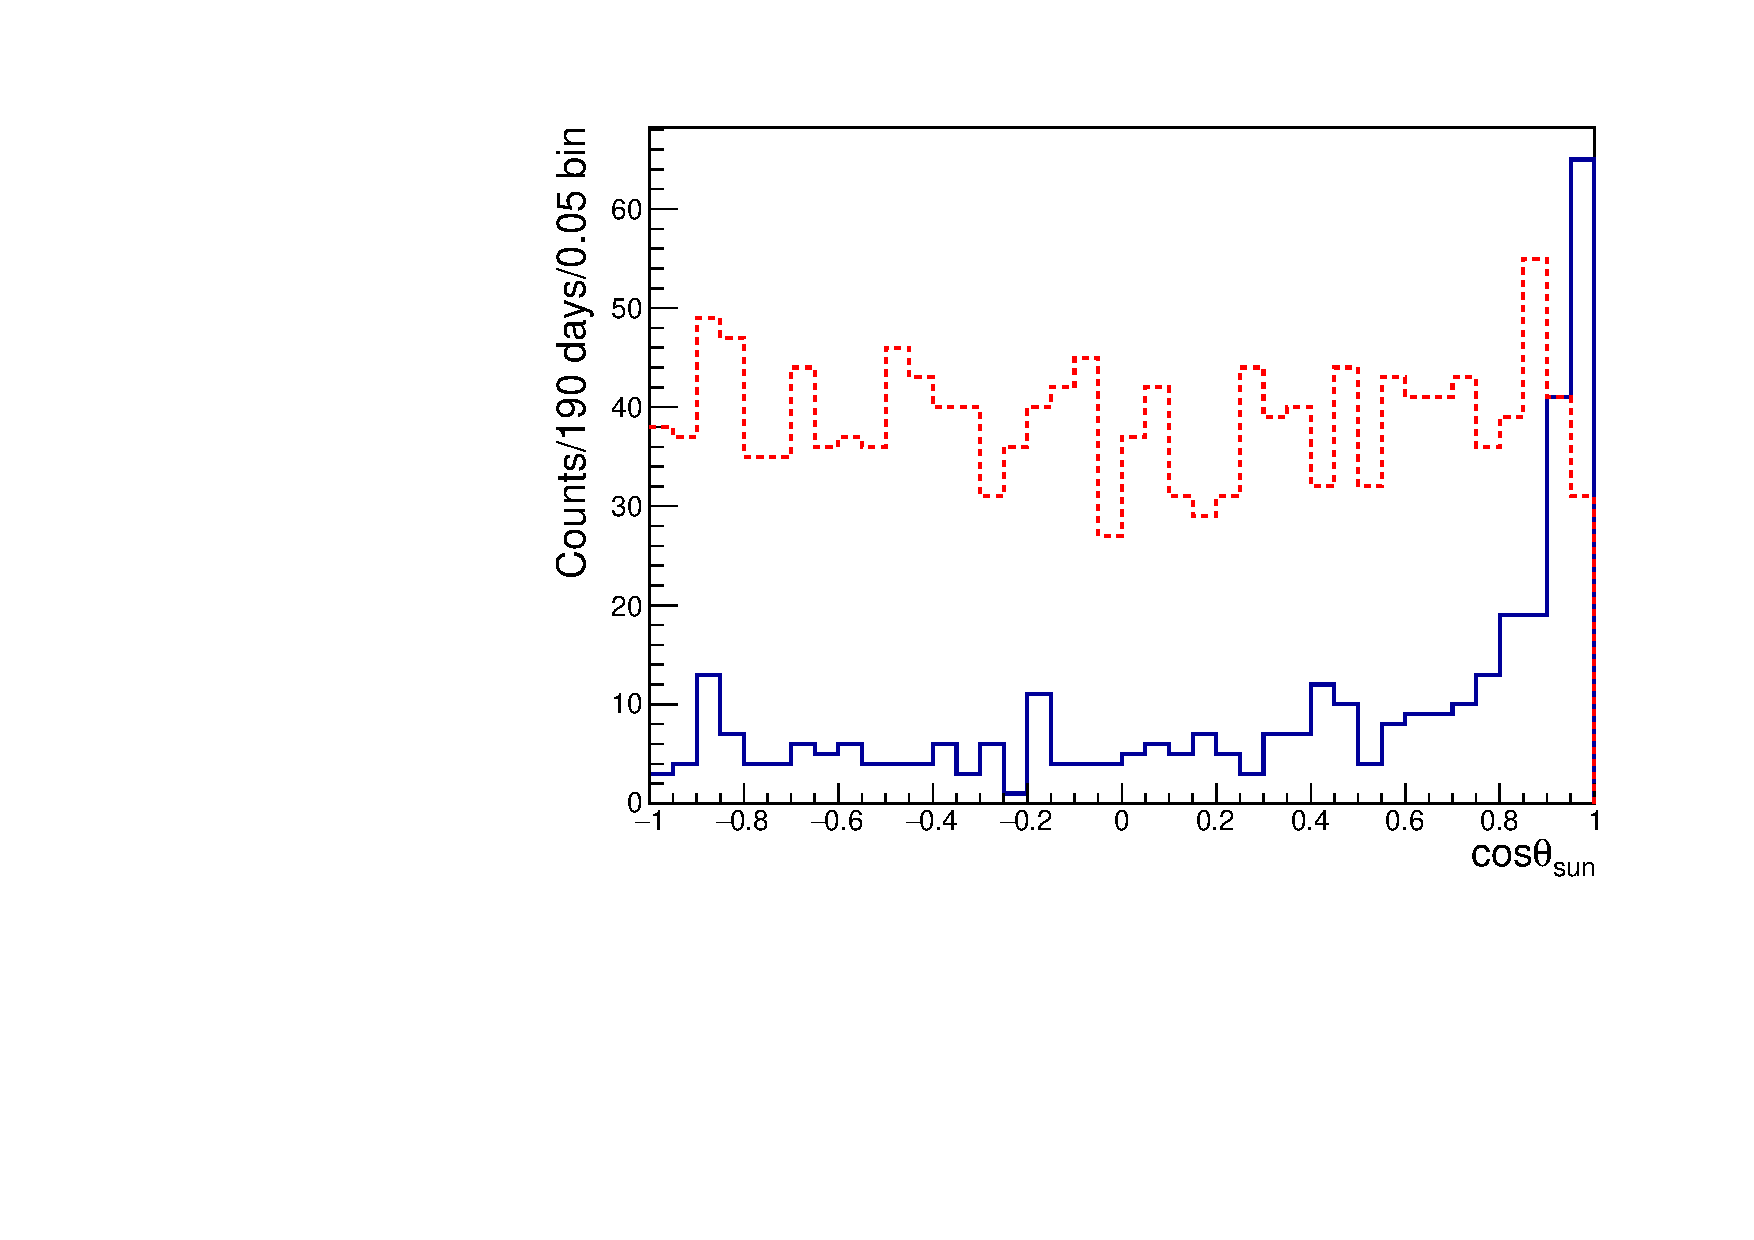
\includegraphics[width=8cm]{cosThetaToSun_4to15_BDT.pdf}
	\caption[BDT output for $\cos\theta_{sun}$, with $4<E_{fit}<15$ MeV.]{BDT output for $\cos\theta_{sun}$, with $4<E_{fit}<15$ MeV. The solid blue line shows the selected candidate solar $\nu_e$ events while the dotted red line shows the selected background events.}
	\label{cosThetaToSun_4to15_BDT}
\end{figure}

\begin{figure}[!htb]
	\centering
	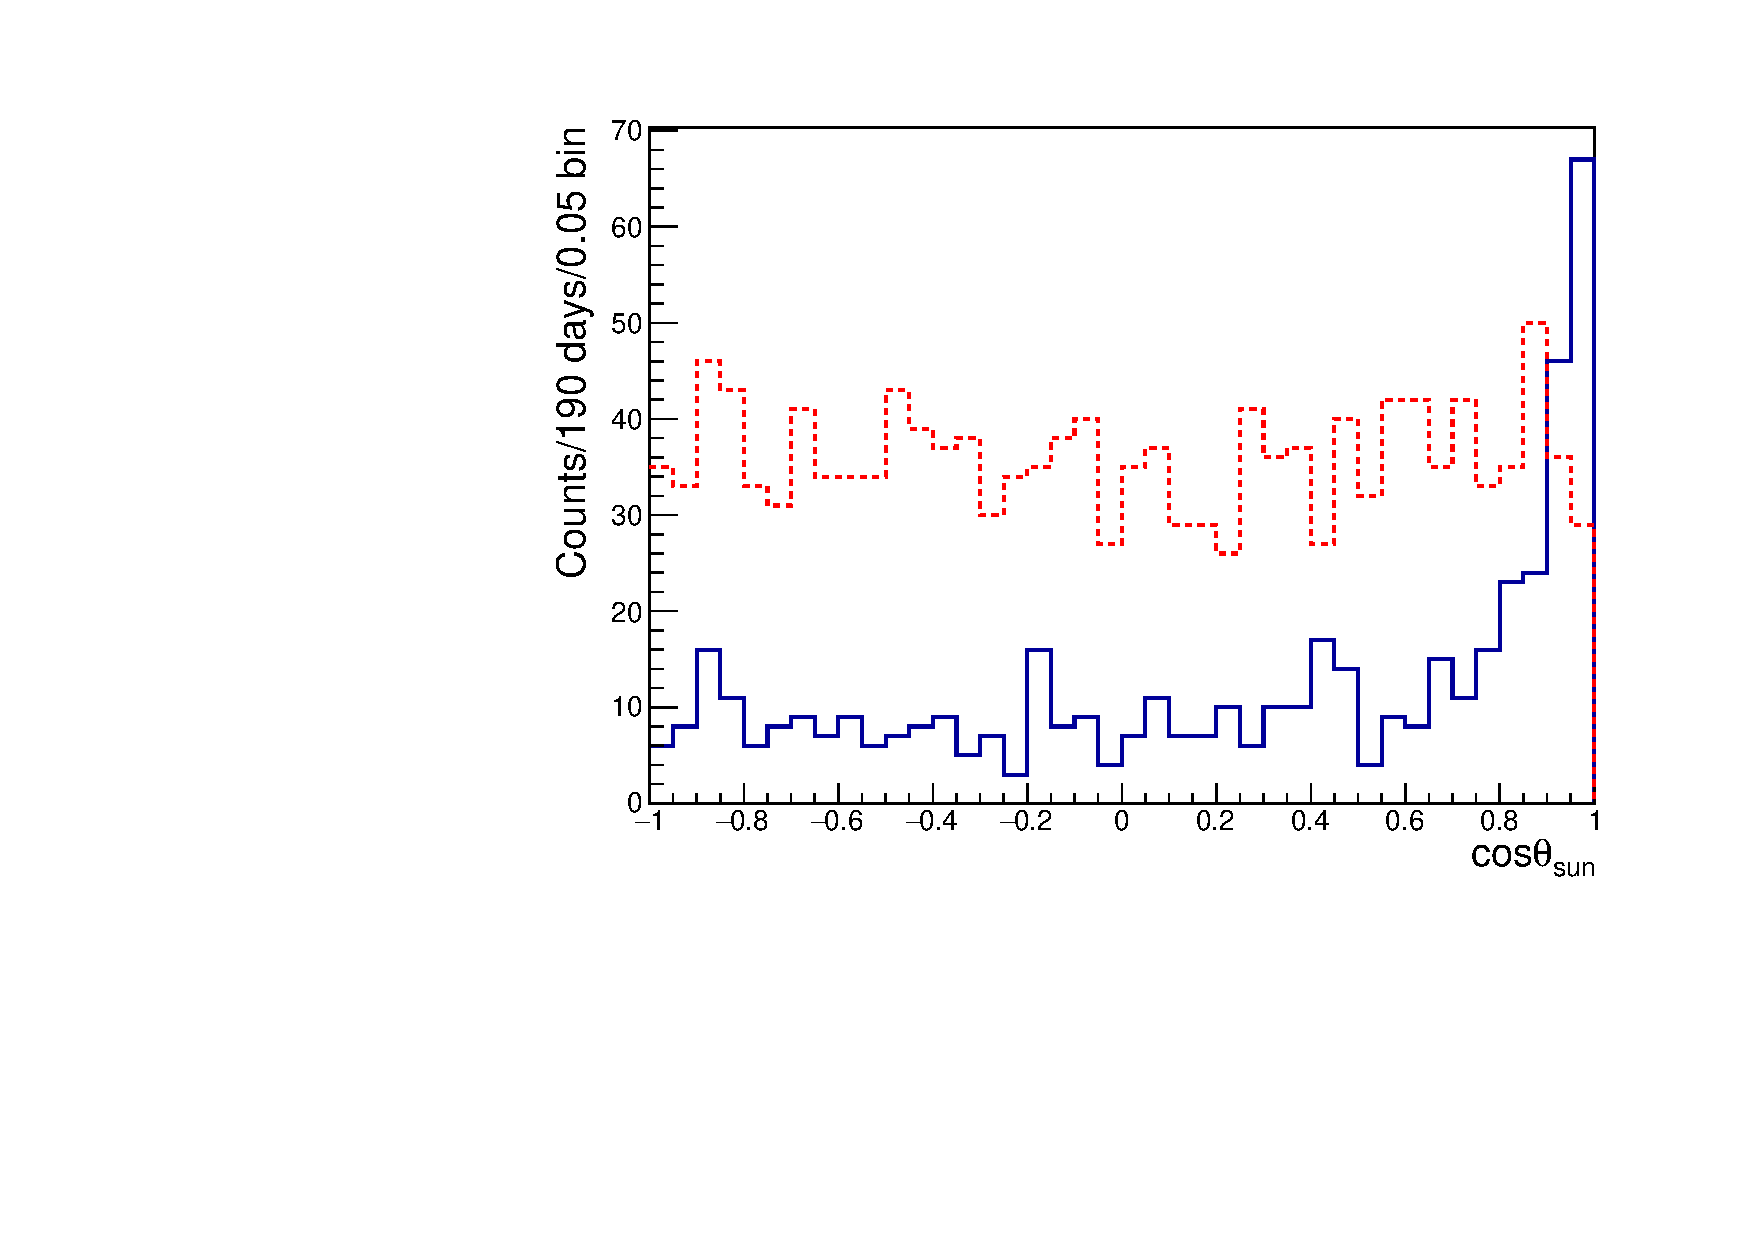
\includegraphics[width=8cm]{cosThetaToSun_4to15_MLP.pdf}
	\caption[MLP output for $\cos\theta_{sun}$, with $4<E_{fit}<15$~MeV.]{MLP output for $\cos\theta_{sun}$, with $4<E_{fit}<15$~MeV. The solid blue line shows the selected candidate solar $\nu_e$ events while the dotted red line shows the selected background events.}
	\label{cosThetaToSun_4to15_MLP}
\end{figure}

\begin{figure}[!htb]
	\centering
	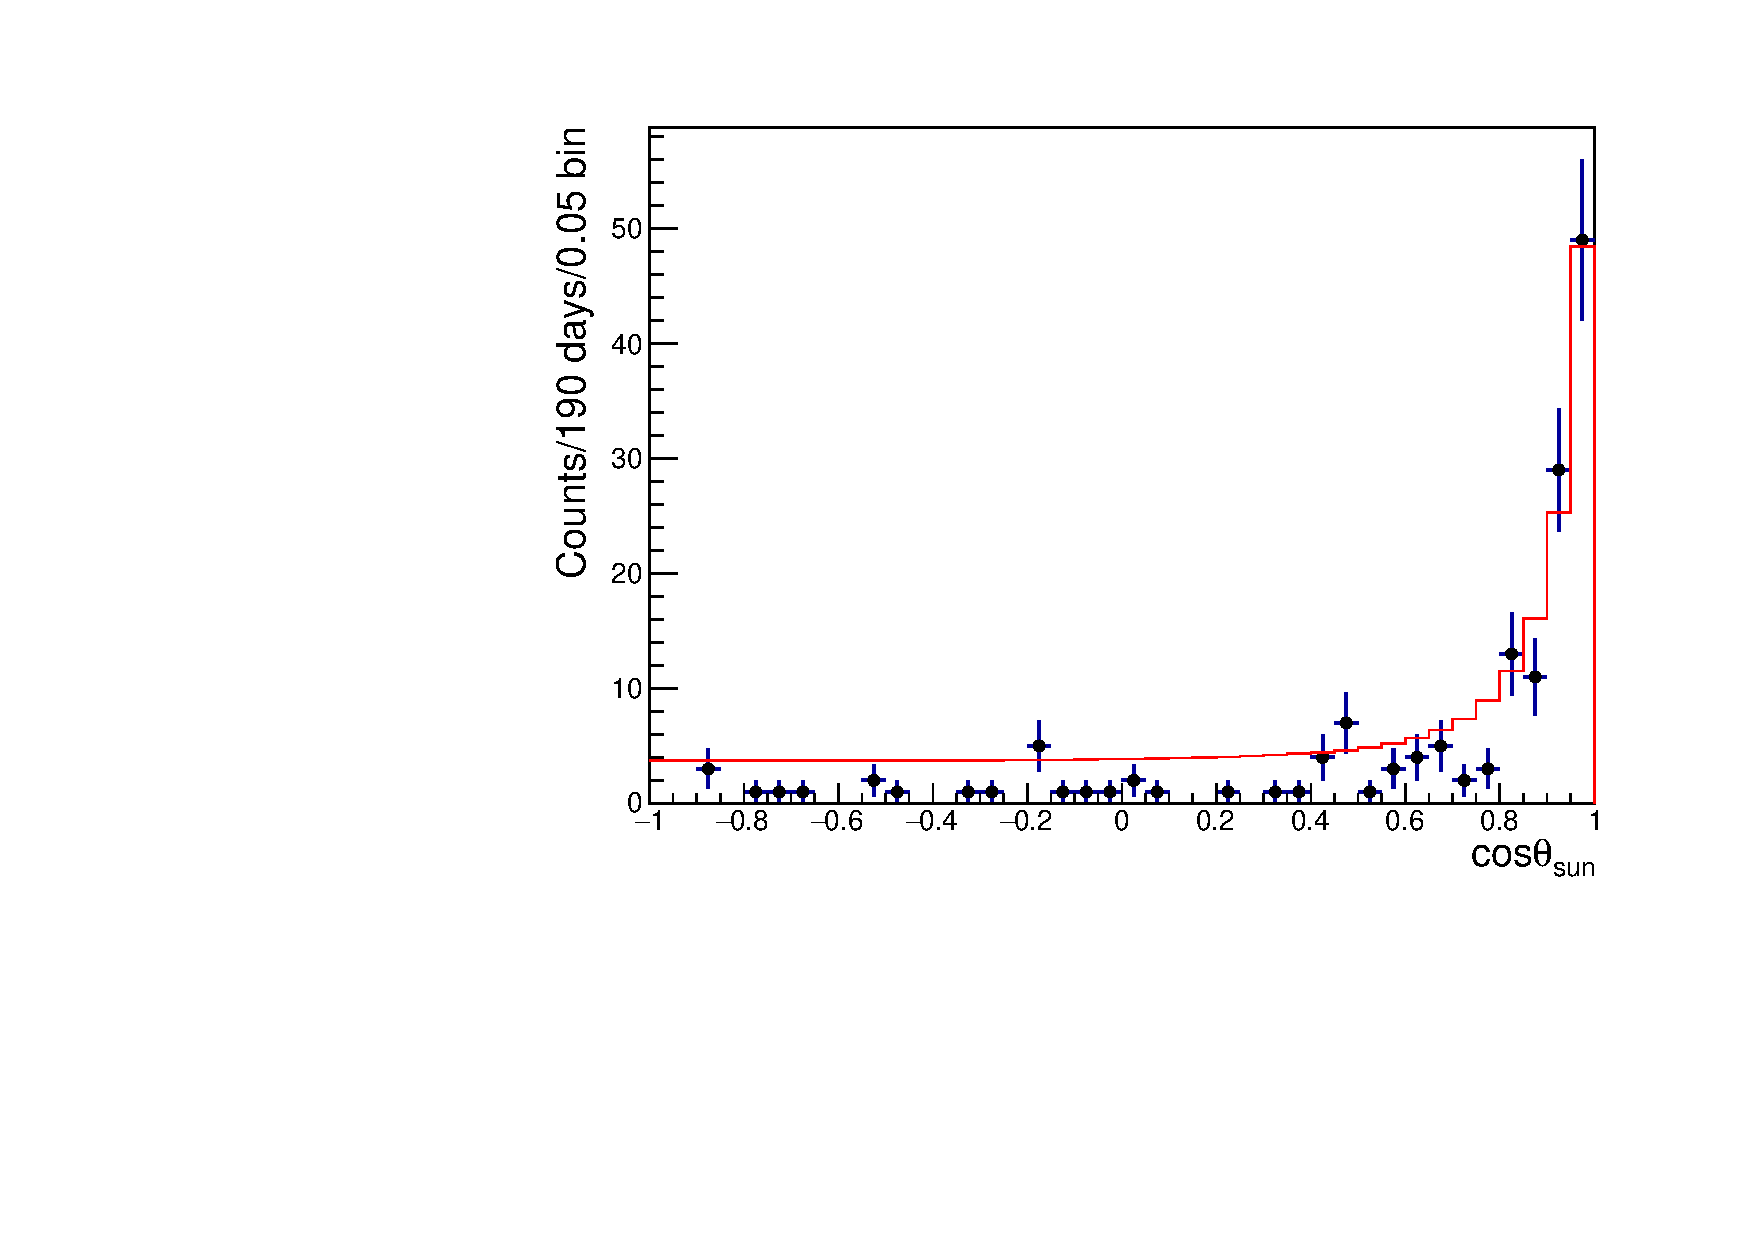
\includegraphics[width=8cm]{cosThetaToSun_5to15_BDT.pdf}
	\caption[BDT output for $\cos\theta_{sun}$, with $4<E_{fit}<15$ MeV.]{BDT output for $\cos\theta_{sun}$, with $4<E_{fit}<15$ MeV. The solid blue line shows the selected candidate solar $\nu_e$ events while the dotted red line shows the selected background events.}
	\label{cosThetaToSun_5to15_BDT}
\end{figure}

\begin{figure}[!htb]
	\centering
	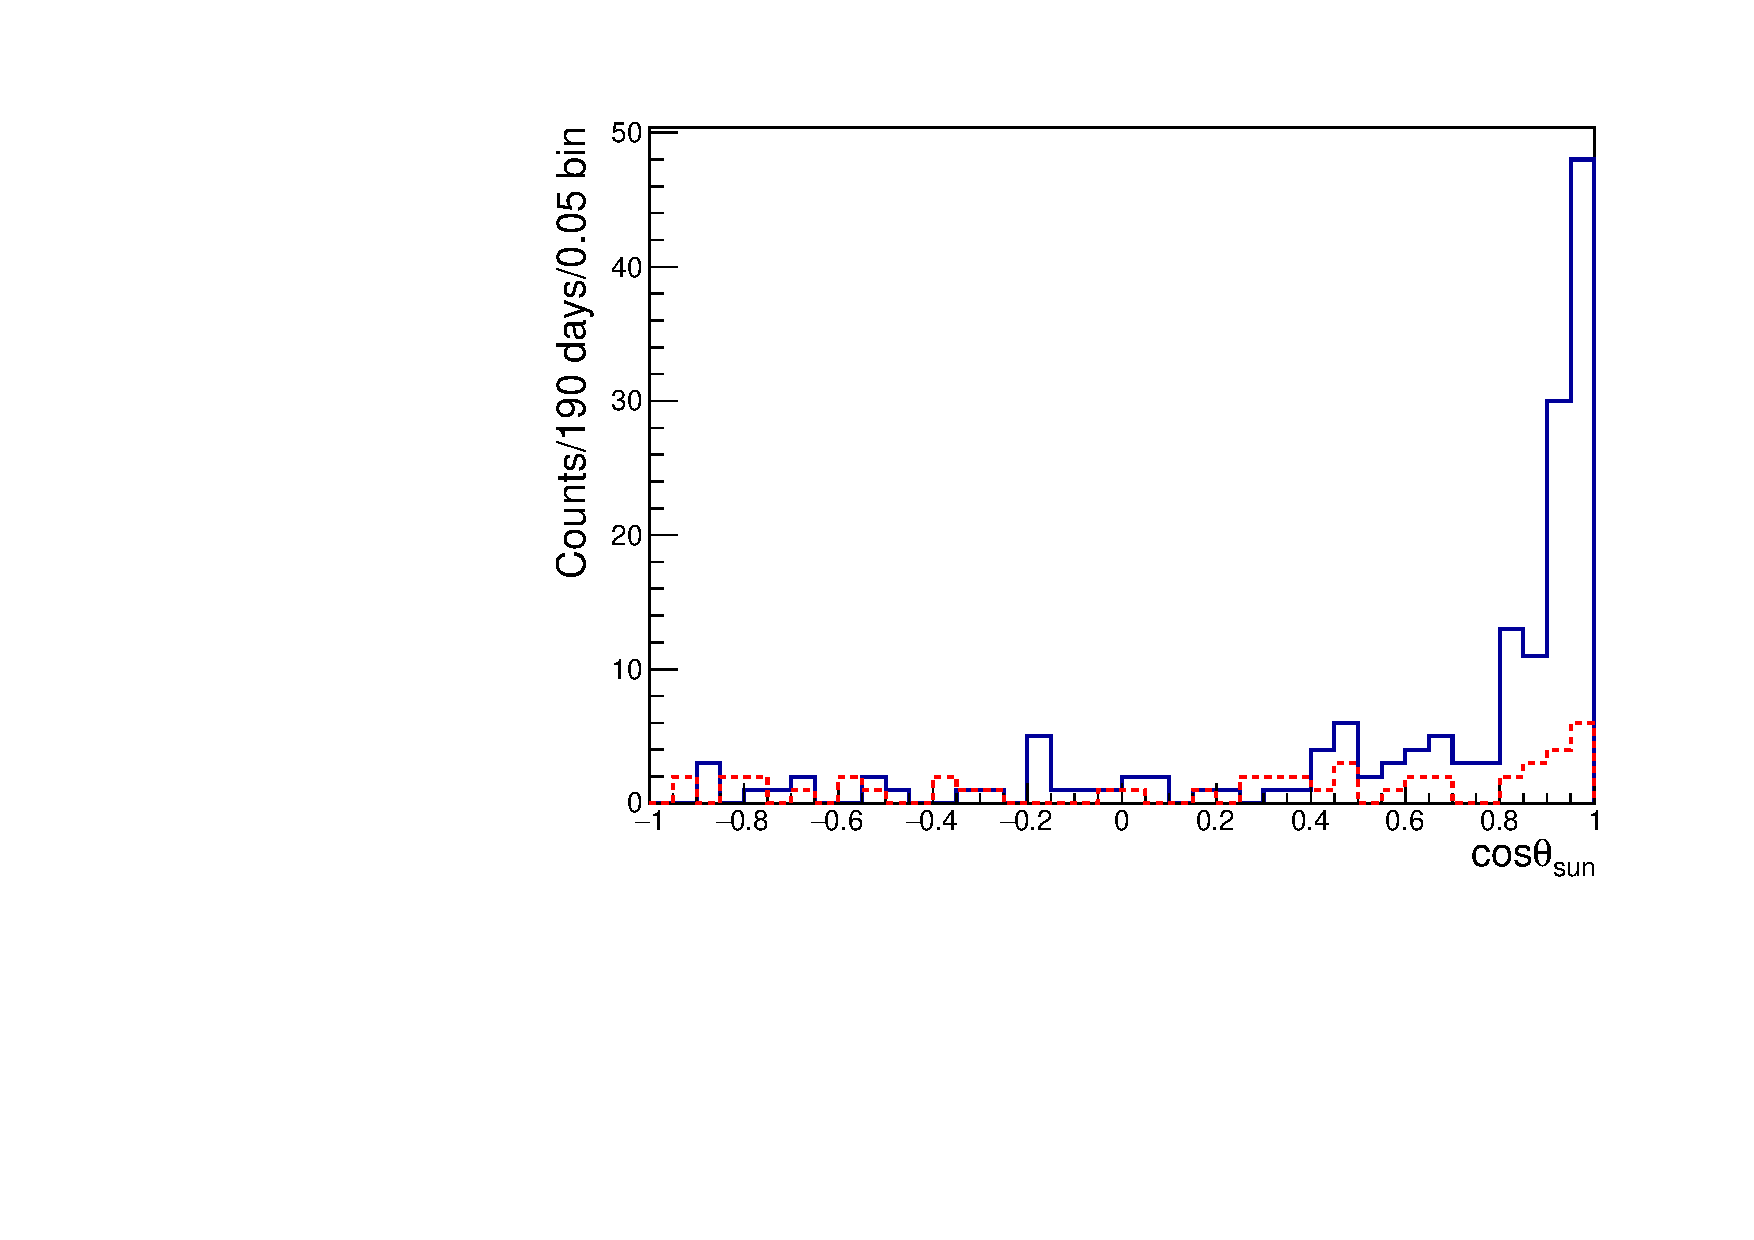
\includegraphics[width=8cm]{cosThetaToSun_5to15_MLP.pdf}
	\caption[MLP output for $\cos\theta_{sun}$, with $5<E_{fit}<15$ MeV.]{MLP output for $\cos\theta_{sun}$, with $5<E_{fit}<15$ MeV. The solid blue line shows the selected candidate solar $\nu_e$ events while the dotted red line shows the selected background events.}
	\label{cosThetaToSun_5to15_MLP}
\end{figure}

%6<E_{fit}<15~MeV$

%Comparisons

The main analysis of this thesis is focused on the [5,15] MeV energy region. A comparison of the outputs of $5<E_{fit}<15$~MeV from the BDT, MLP and the default cuts is shown in Fig.~\ref{compare_cosThetaToSun_5to15}.
\begin{figure}[!htb]
	\centering
	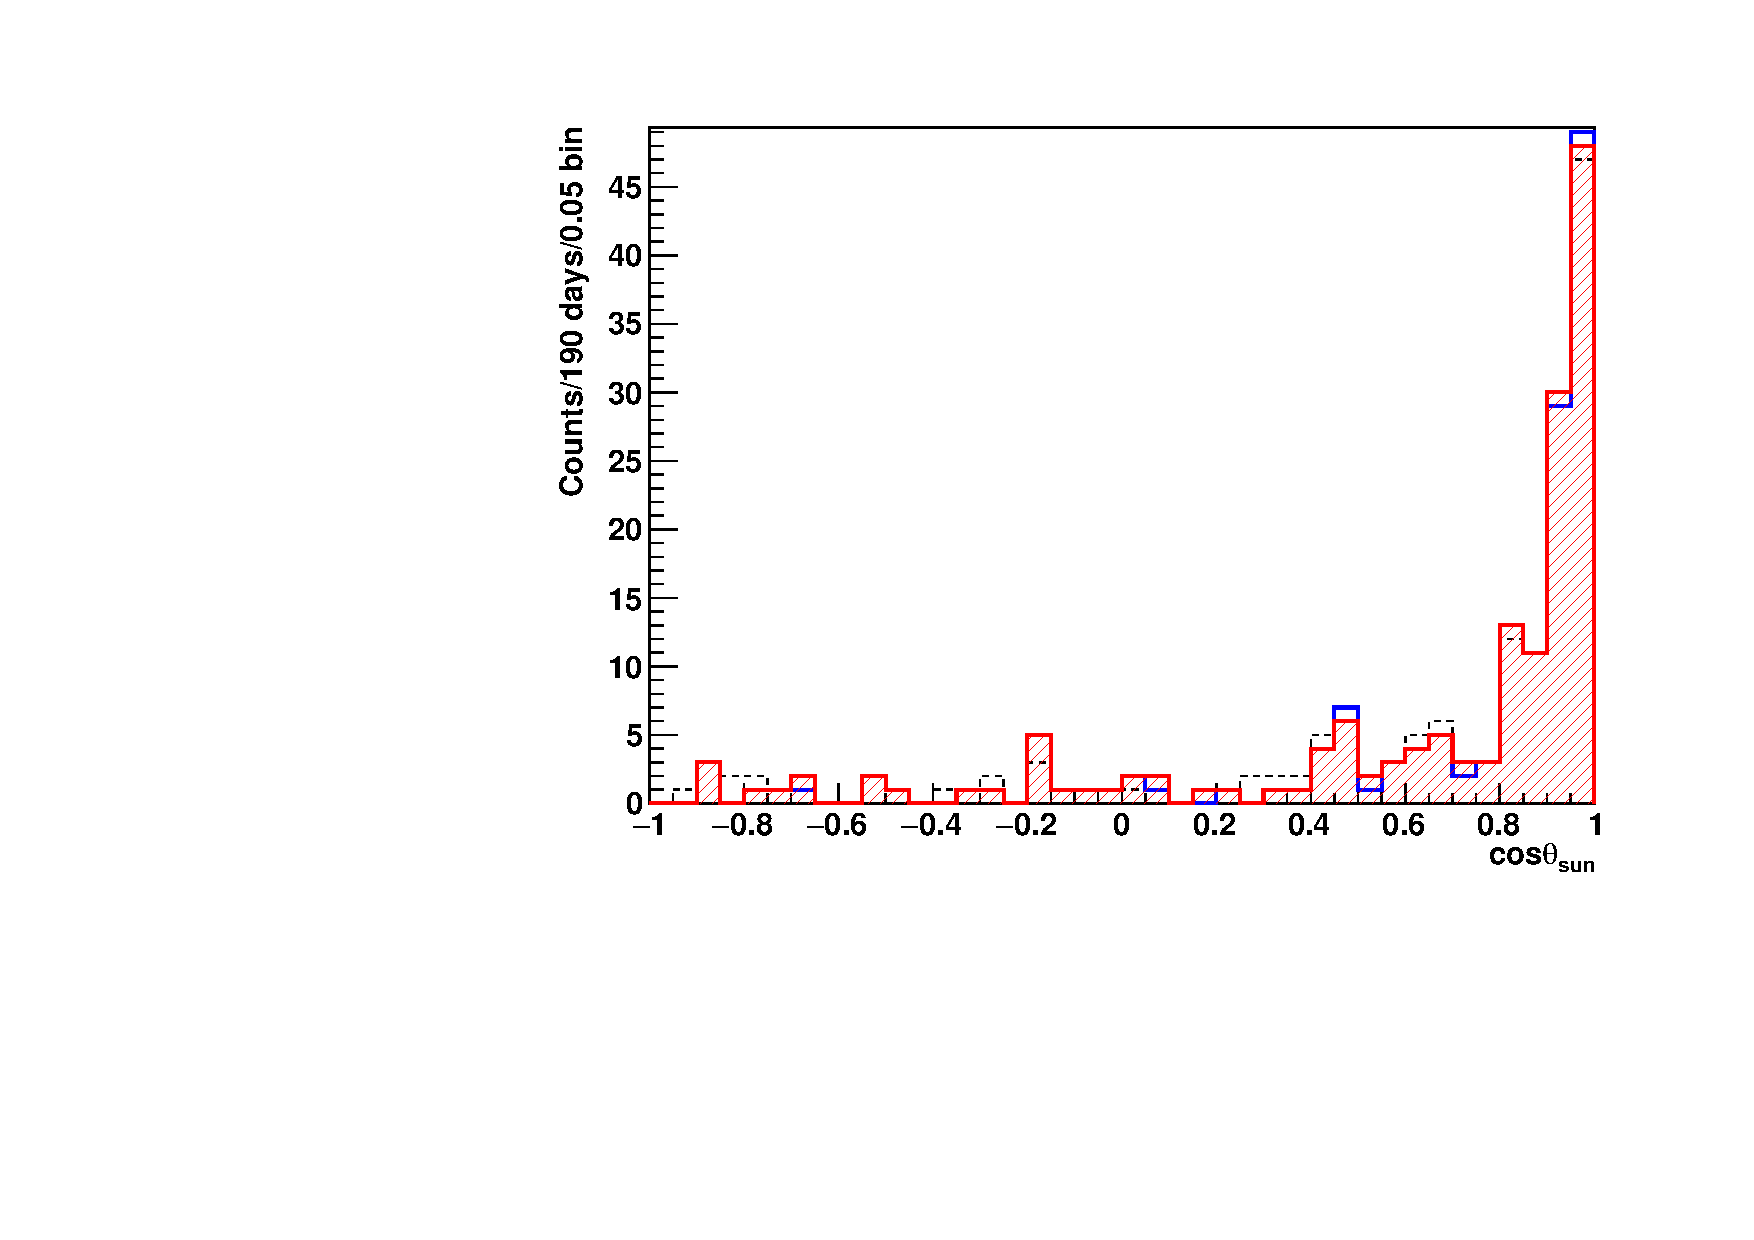
\includegraphics[width=8cm]{Compare_cosThetaSun_5to15.pdf}
	\caption[A comparison of the outputs of the BDT, MLP and the default cuts for the $5<E_{fit}<15$ MeV.]{A comparison of the outputs of the BDT, MLP and the default cuts for the $5<E_{fit}<15$ MeV. The solid blue line shows the BDT results; the red slashes show the MLP results and the dotted black line shows the default cut results.}
	\label{compare_cosThetaToSun_5to15}
\end{figure}

\subsection{Discussions on the TMVA Results}
A more stringent radial cut (or tighter FV) can be applied on lower energy region $4<E_{fit}<5$~MeV to further remove the background events which are dominant in lower energy region. However, this tighter cut can also reduce the signal events.

Other packages developed for high energy particle physics, such as \texttt{StatPatternRecognition} (SPR)\cite{sprWebsite}, can also be considered as an alternative tool or as a reference for results comparisons. 

\subsection{Likelihood Fits for Solar Neutrino Candidate Events}
In the previous section, the optimized cuts obtained from the TMVA analysis were applied on the dataset. 

After the event selections, a distribution of $\cos\theta_{sun}$ extracted from the solar $\nu_e$ candidate events was obtained. 

\subsubsection{Maximum Likelihood Fit}\label{sect:poisson_fit}
A maximum likelihood method was applied on the distribution to extract the number of the solar $\nu_e$ interaction events ($N_{sig}$) as well as the number of the background events ($N_{bkg}$).

The values of $\cos\theta_{sun}$ from the selected events were filled into a histogram divided into bins.
For each bin, the observed event number ($n_{obs}$) was considered as a sum of solar $\nu_e$ and background events. The $n_{obs}$ in each bin was assumed to follow a Poisson distribution: $Poisson(n_{obs}, N_{bkg}\cdot P_{bkg}+N_{sig}\cdot P_{ES}(E))$, where $P_{bkg}$ and $P_{ES}(E)$ are the assumed distribution of backgrounds and solar $\nu_e$ events respectively.

For the background events, a uniform distribution of $\cos\theta_{sun}$ was assumed. On the other hand, the $\cos\theta_{sun}$ distributions of solar $\nu_e$ were extracted from the realistic run simulations after applying the optimized cuts, as shown in Fig.~\ref{solarPDF}. 

\begin{figure}[!htb]
	\centering
	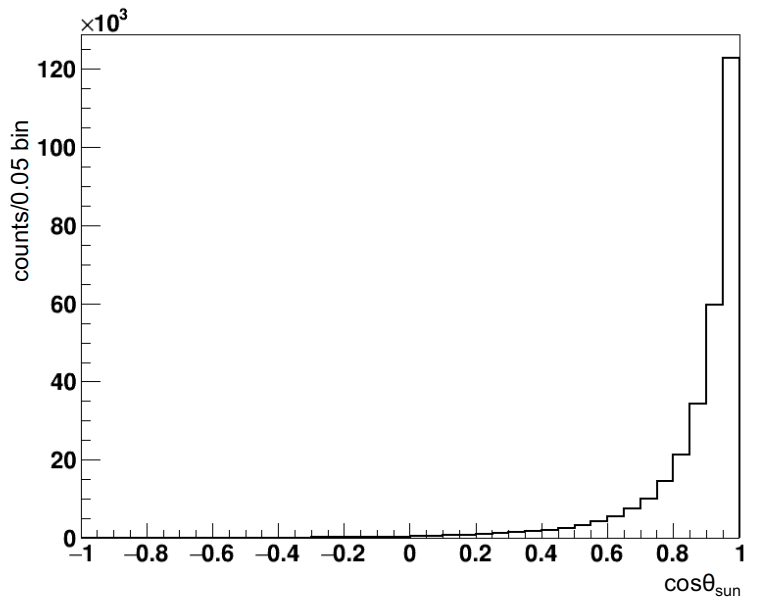
\includegraphics[width=10cm]{solarPDF.png}
	\caption{The $\cos\theta_{sun}$ distribution of solar $\nu_e$ extracted from the simulations, which was used as a $PDF$ function.}
	\label{solarPDF}
\end{figure}

Adding up each bin $i$ and taking $N_{bkg}$ and $N_{sig}$ as the free parameters for fitting, the maximum likelihood function was built as\cite{pdg2020}:
%\begin{equation}\label{eq:solar_poissonFit}
%-\ln\mathcal L(N_{sig},N_{bkg}|n_{obs})
%=-\sum_i^{N_{bins}}\ln(Poisson(n^i_{obs}, N_{bkg}P^i_{bkg}+N_{sig}P^i_{ES}(E^i))).
%\end{equation}

\begin{equation}\label{eq:solar_poissonFitMinimizer}
-2\ln\mathcal \lambda(N_{sig},N_{bkg})
=2\sum_{i=0}^{N_{bins}}[\mu_i(N_{sig},N_{bkg})-n_i+n_i\ln\frac{n_i}{\mu_i(N_{sig},N_{bkg})}],
\end{equation}
where $\mu_i(N_{sig},N_{bkg})$ is the expected number of events in each bin: $\mu_i(N_{sig},N_{bkg})=N_{sig}\cdot P^i_{ES}(E^i)+N_{bkg}\cdot1/N_{bins}$; $N_{bins}$ is the total number of the bins, usually taken as 40 (per 0.05 bins). This quantity also includes the cases when the bin contains zero ($n_i=0$).

Fitting the data with $(N_{bkg},N_{sig})$ by maximizing the quantity \ref{eq:solar_poissonFitMinimizer}, $N_{bkg}$ and $N_{sig}$ were obtained. In the next section, an ensemble test based on fake datasets was used for testing the fit results.
%Fig.~\ref{solarFits1} shows the fit results. The fitted number of solar $\nu_e$ events is $N_{sig} = 67.1\pm9.2$, which is equivalent to a rate of $1.04\pm 0.14~event/(day\cdot kiloton)$; while the fitted number of background events is $N_{sig} = 3.4\pm0.91$, which is equivalent to a rate of $0.05\pm 0.01 event/(day\cdot kiloton)$.
%
%\begin{figure}[!htb]
%	\centering
%	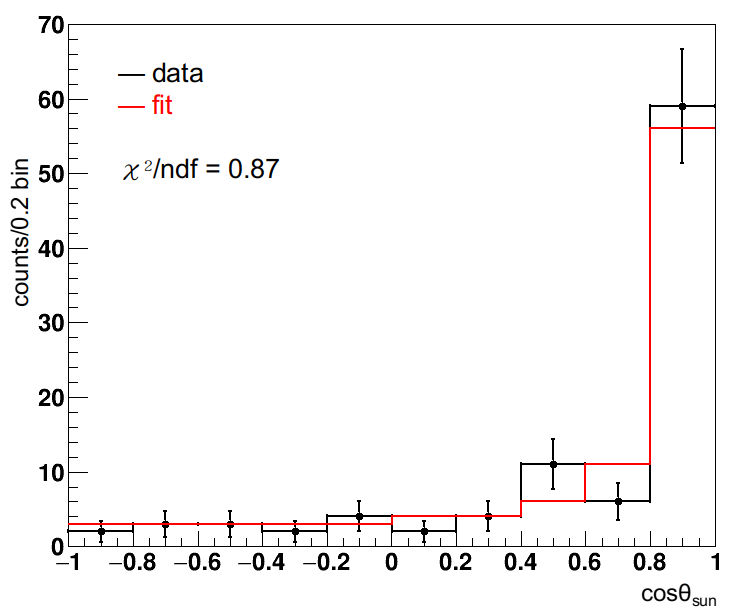
\includegraphics[width=8cm]{solarFits1.png}
%	\caption{Fitted results for the $N_{bkg}$ and $N_{sig}$ via the maximum likelihood method.}
%	\label{solarFits1}
%\end{figure}
%
%2D fits
\subsubsection{Ensemble Test}
To check the uncertainty of the Poisson fit, 5000 fake datasets were generated. Here I used the method similar to the Ref.~\cite{leta}.
The fake data were taken from the run-by-run MC simulations of the run-200004 to 203602, which has 92.54 live days. The default cuts mentioned in the last section were applied on these simulations.
%In the MC dataset, for $E_{fit}>5~MeV$, there were 6359 backgrounds from different background events and 317205 signals of internal solar $\nu_e$ events (the event types were mentioned in Table.~\ref{table:mixed_MC}).

The number of backgrounds in a fake dataset, $N^f_{bkg}$, was assumed to be two times of the event number in the $-1<\cos\theta_{sun}<0$ region while the number of signals $N^f_{sig}=N^f_{total}-N^f_{bkg}$. Reading from the sub-dataset of run-200004 to 203602, it found $N^f_{bkg}=38$ and then $N^f_{sig}=109-N^f_{bkg}=71$, as shown in Fig.~\ref{half_data}. To do the ensemble test, for each fake dataset, two random numbers: $N^r_{sig}$ and $N^r_{bkg}$ were generated by the $\texttt{ROOT TRandom3}$ random number generator class. Each of the two random numbers followed the random Poisson distribution: $e^{-\mu}\mu^{N^r}/N^r!$, where $\mu=71$ or $38$, and thus they fluctuated around $N^f_{sig}$ or $N^f_{bkg}$.

\begin{figure}[!htb]
	\centering
	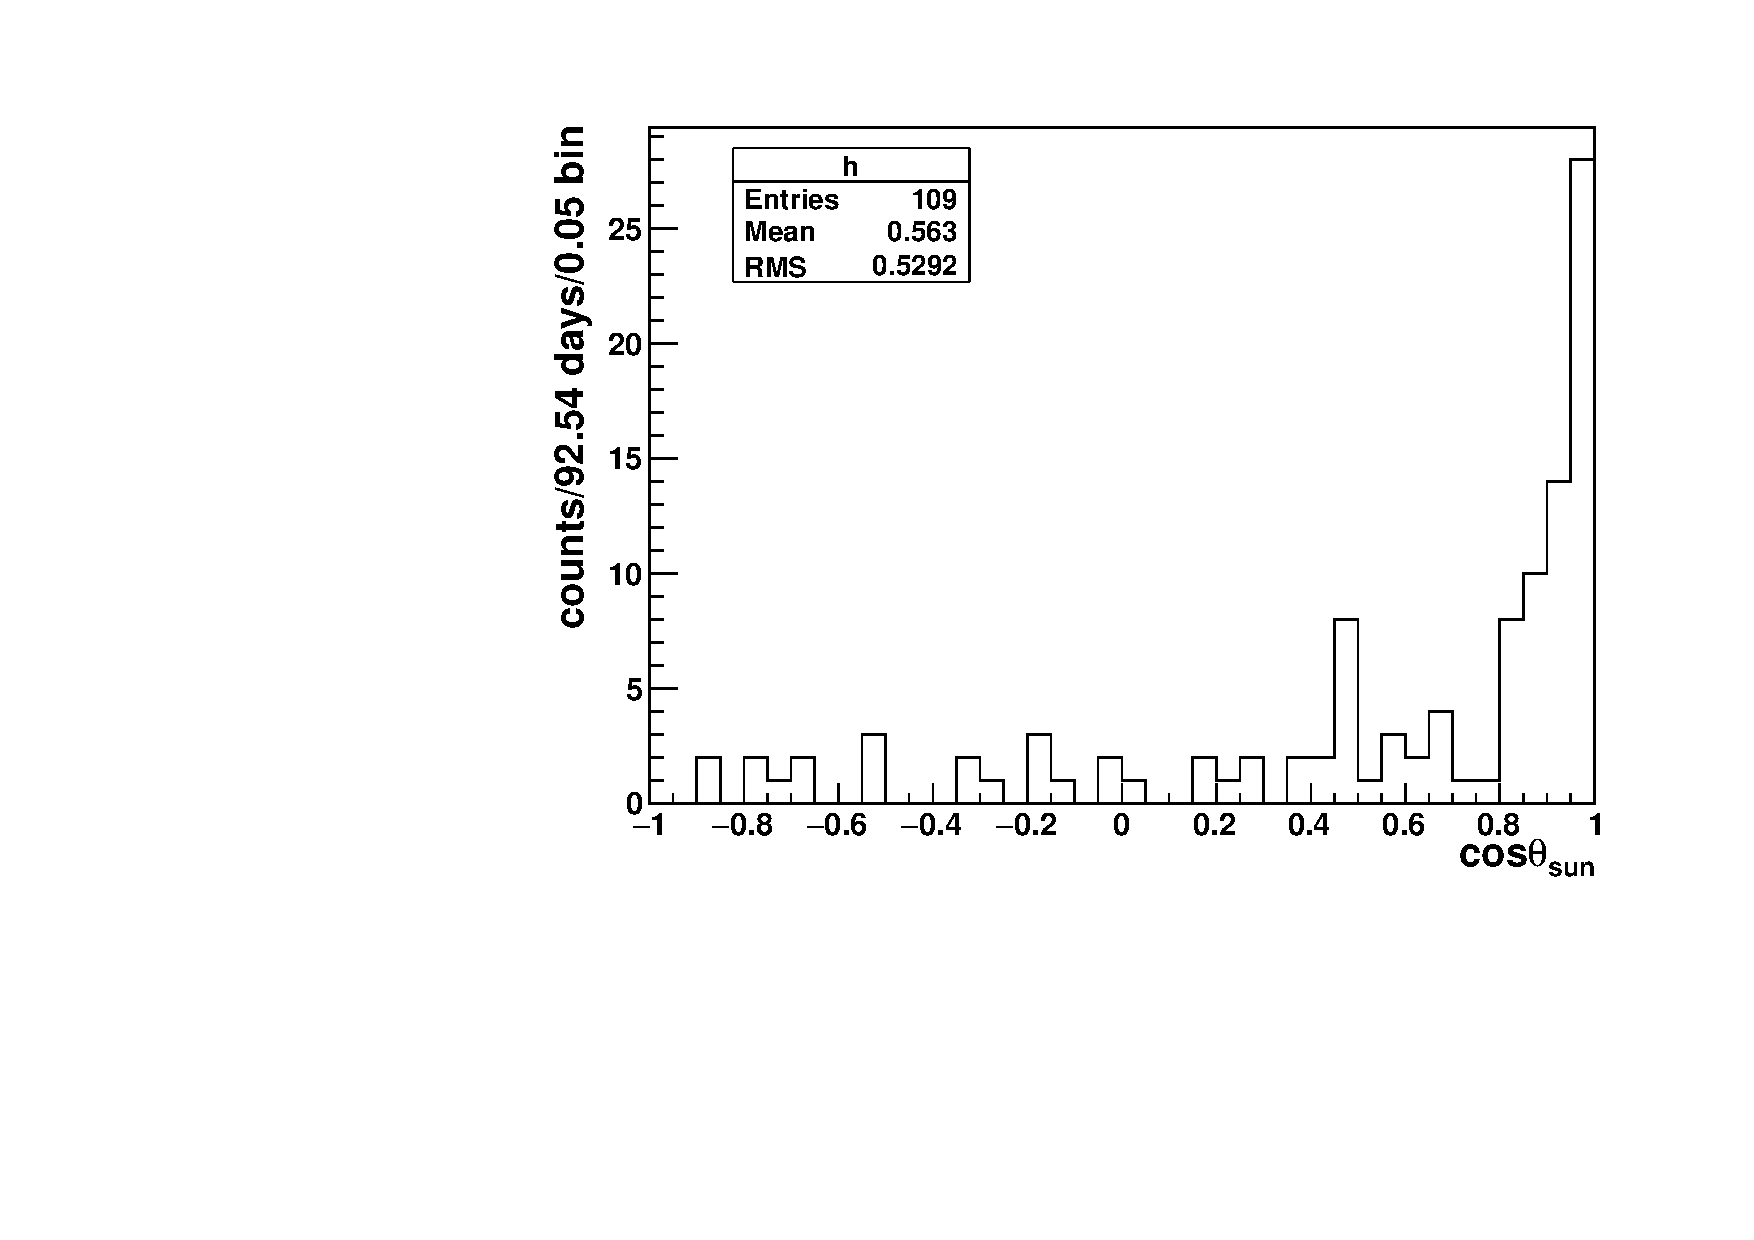
\includegraphics[width=10cm]{cosThetaToSun_halfData_5to15.pdf}
	\caption[Real data from run-200004 to 203602 (``half dataset''), after the default cuts.]{Real data from run-200004 to 203602 (half dataset), after the default cuts. The number of counts in $-1<\cos\theta_{sun}<0$ region is 19.}
	\label{half_data}
\end{figure}

To create the fake datasets, $N^r_{sig}$ ($N^r_{bkg}$) events after the cuts were randomly and uniformly selected from the solar $\nu_e$ (merged backgrounds) MC simulations. For each randomly selected event, the values of $E_{fit}$ and $\cos\theta_{sun}$ were recorded. Each dataset was fitted with the maximum likelihood function described in Sect.~\ref{sect:poisson_fit}. Fig.~\ref{ensemble_test} shows an example of the fitted results.

\begin{figure}[!htb]
	\centering
	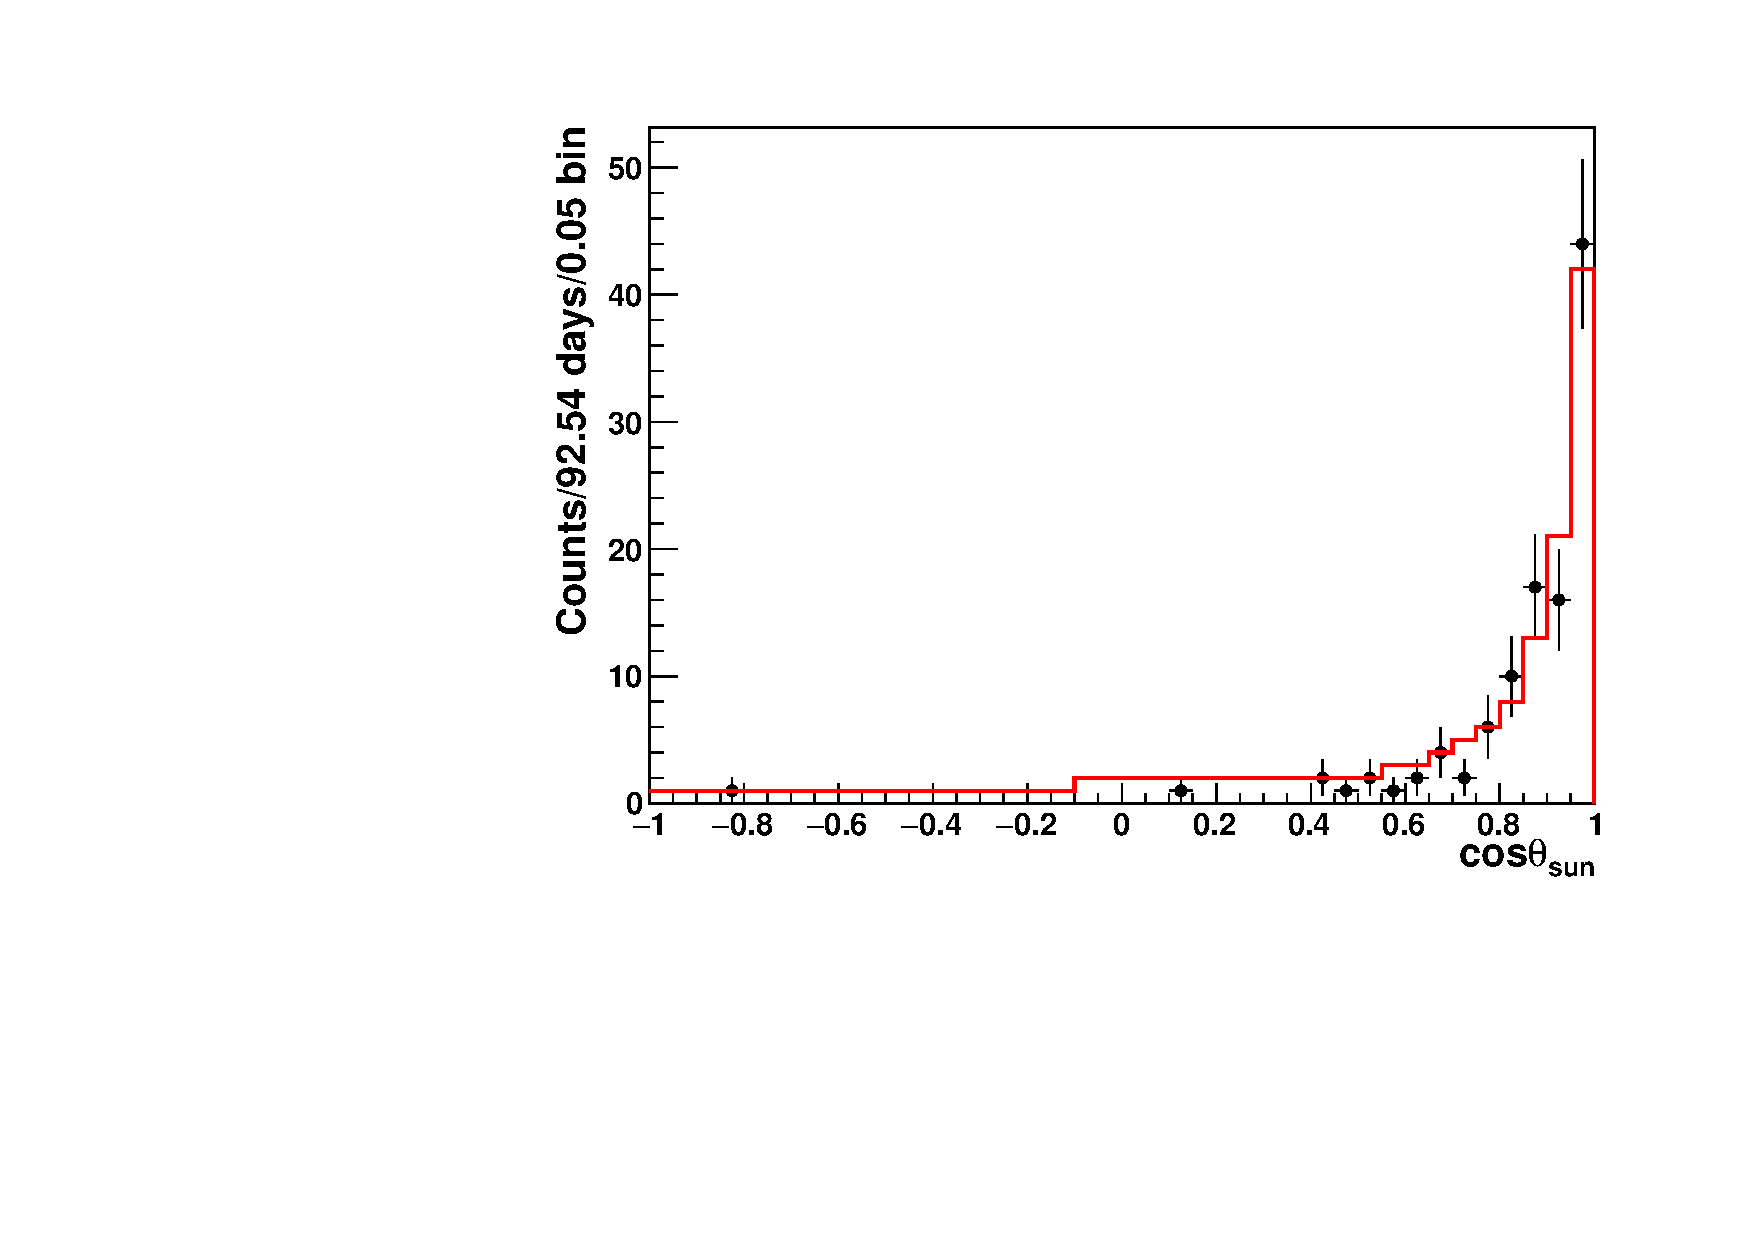
\includegraphics[width=10cm]{ensemble_fitExample.pdf}
	\caption[An example of the randomly generated $\cos\theta_{sun}$ fitted with $(N_{sig},N_{bkg})$.]{An example of the randomly generated $\cos\theta_{sun}$ fitted with $(N_{sig},N_{bkg})$. The black dots are data points and the red line is the fitted results. For $N^r_{sig} = 73$ and $N^r_{bkg}=44$, the fitted results give $N_{sig} = 73.42\pm9.42$ and $N_{bkg} = 43.58 \pm 7.73$, with a $\chi^2/ndf = 60.19/40 = 1.50$.}
	\label{ensemble_test}
\end{figure} 

The fit pull and the fit bias were defined by \cite{leta}:
\begin{equation}
bias=\frac{N_{sig}-N^r_{sig}}{N_{sig}},
\end{equation}

\begin{equation}
pull=\frac{N_{sig}-N^r_{sig}}{\sigma_{sig}},
\end{equation}
where $N_{sig}$ is the fitted number of signal events, $\sigma_{sig}$ is the statistical uncertainty of $N_{sig}$; $N^{r}_{sig}$ is used as the true number of signal events in the fake dataset.

Fig.~\ref{poisson_fitPull} and Fig.~\ref{poisson_fitBias} show the fit pull and biases respectively. The histograms were fitted with Gaussians. For the fitted number of signal events, the Gaussian mean of the fit biases is $-0.0044\pm0.0008$ for 5000 fake datasets while the Gaussian mean of the fit pulls is $-0.026\pm0.006$. These pulls and biases will be applied on the data. Fig.~\ref{poisson_fitLnL} shows the distributions of the $-2\ln L$ returned by the best fitted results ($-2\ln L_{best}$). The distribution, $f({-2\ln L_{best}})$, follows the asymptotic $\chi^2$ pdf with a degree of 40 and is used to compute the p-values\cite{pdg2020}. For a best-fit set ($N^i_{sig},N^i_{bkg}$) with a value of $-2\ln L^i_{best}$, the p-value is calculated as $p=\int_{-2\ln L^{i}_{best}}^{-2\ln L^{max}_{best}}f({-2\ln L_{best}})d(-2\ln L_{best})$.

\begin{figure}[!htb]
	\centering
	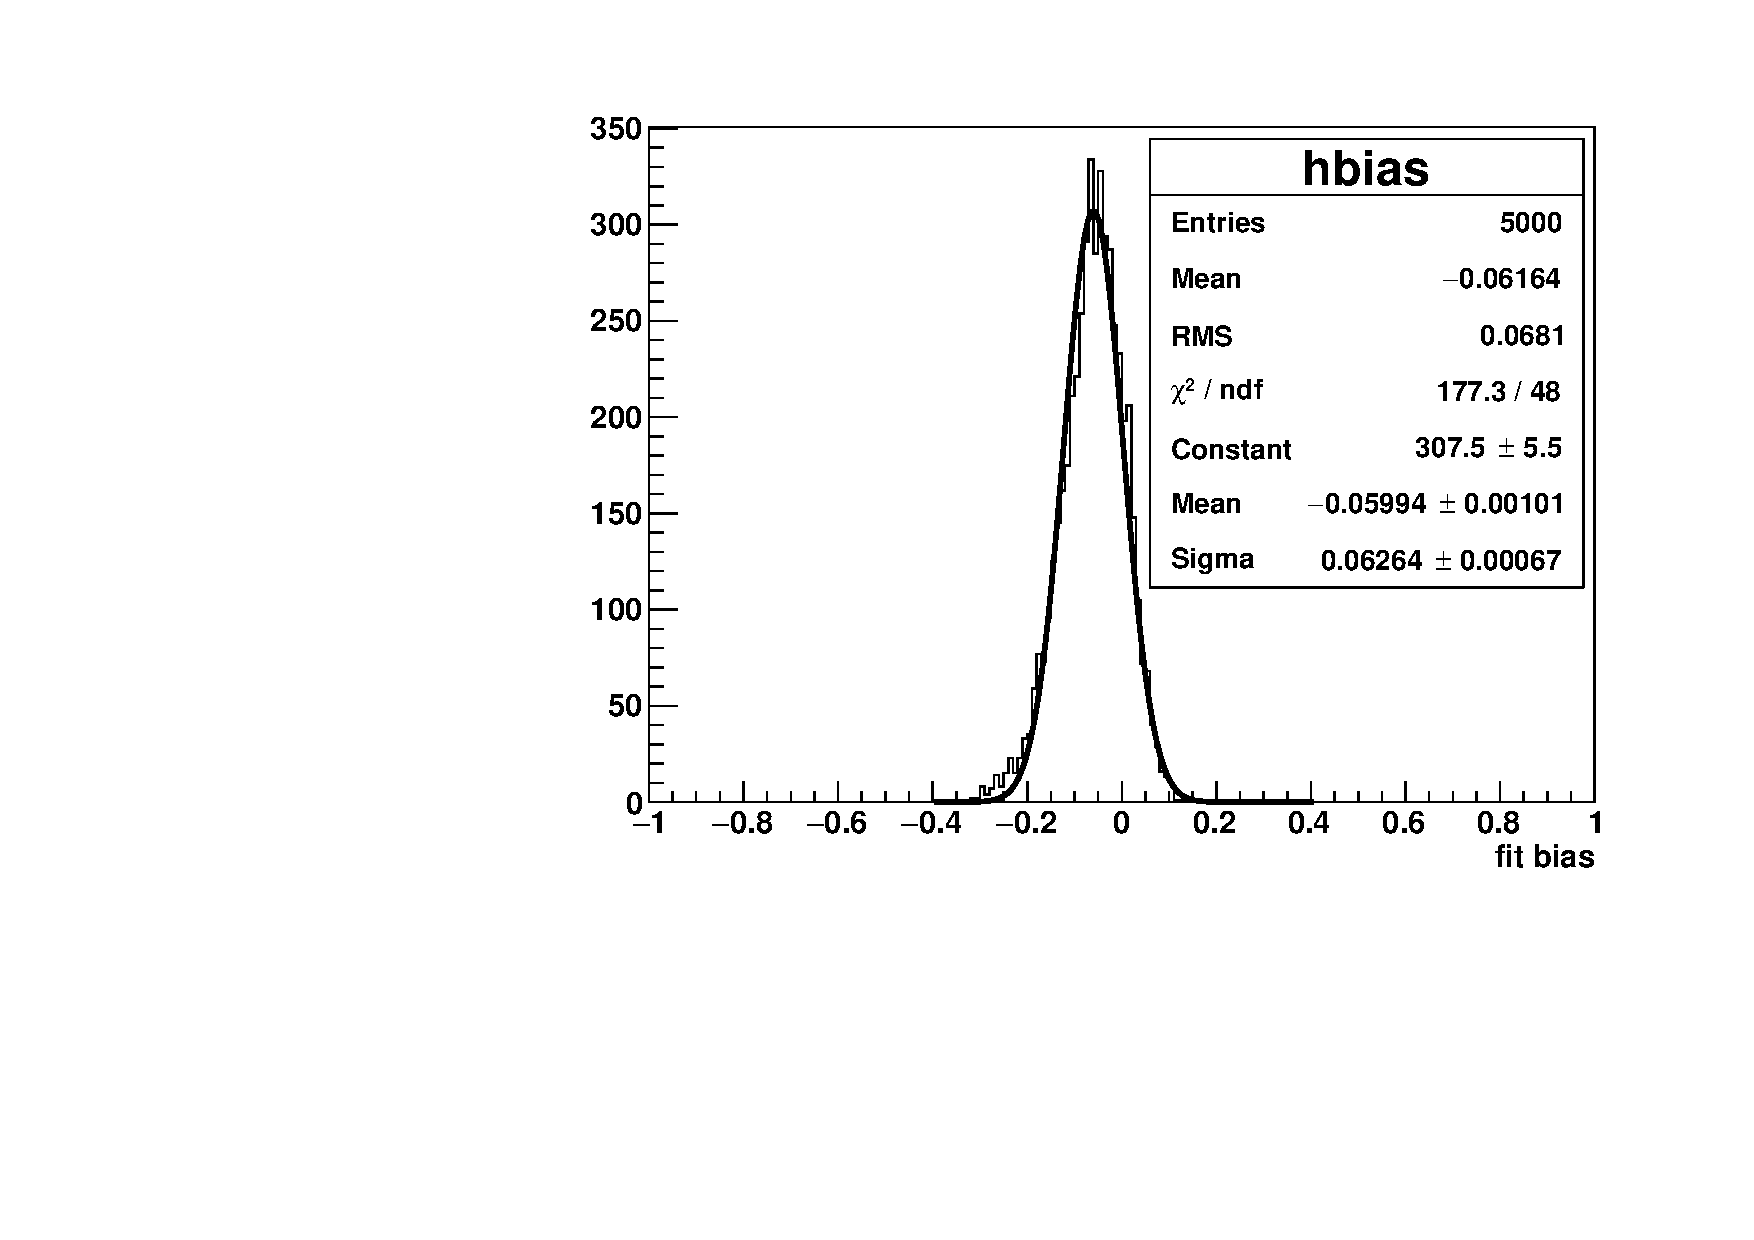
\includegraphics[width=8cm]{ensemble_fitBias.pdf}
	\caption{$N_{sig}$ fit biases for 5000 fake datasets.}
	\label{poisson_fitBias}
\end{figure} 

\begin{figure}[!htb]
	\centering
	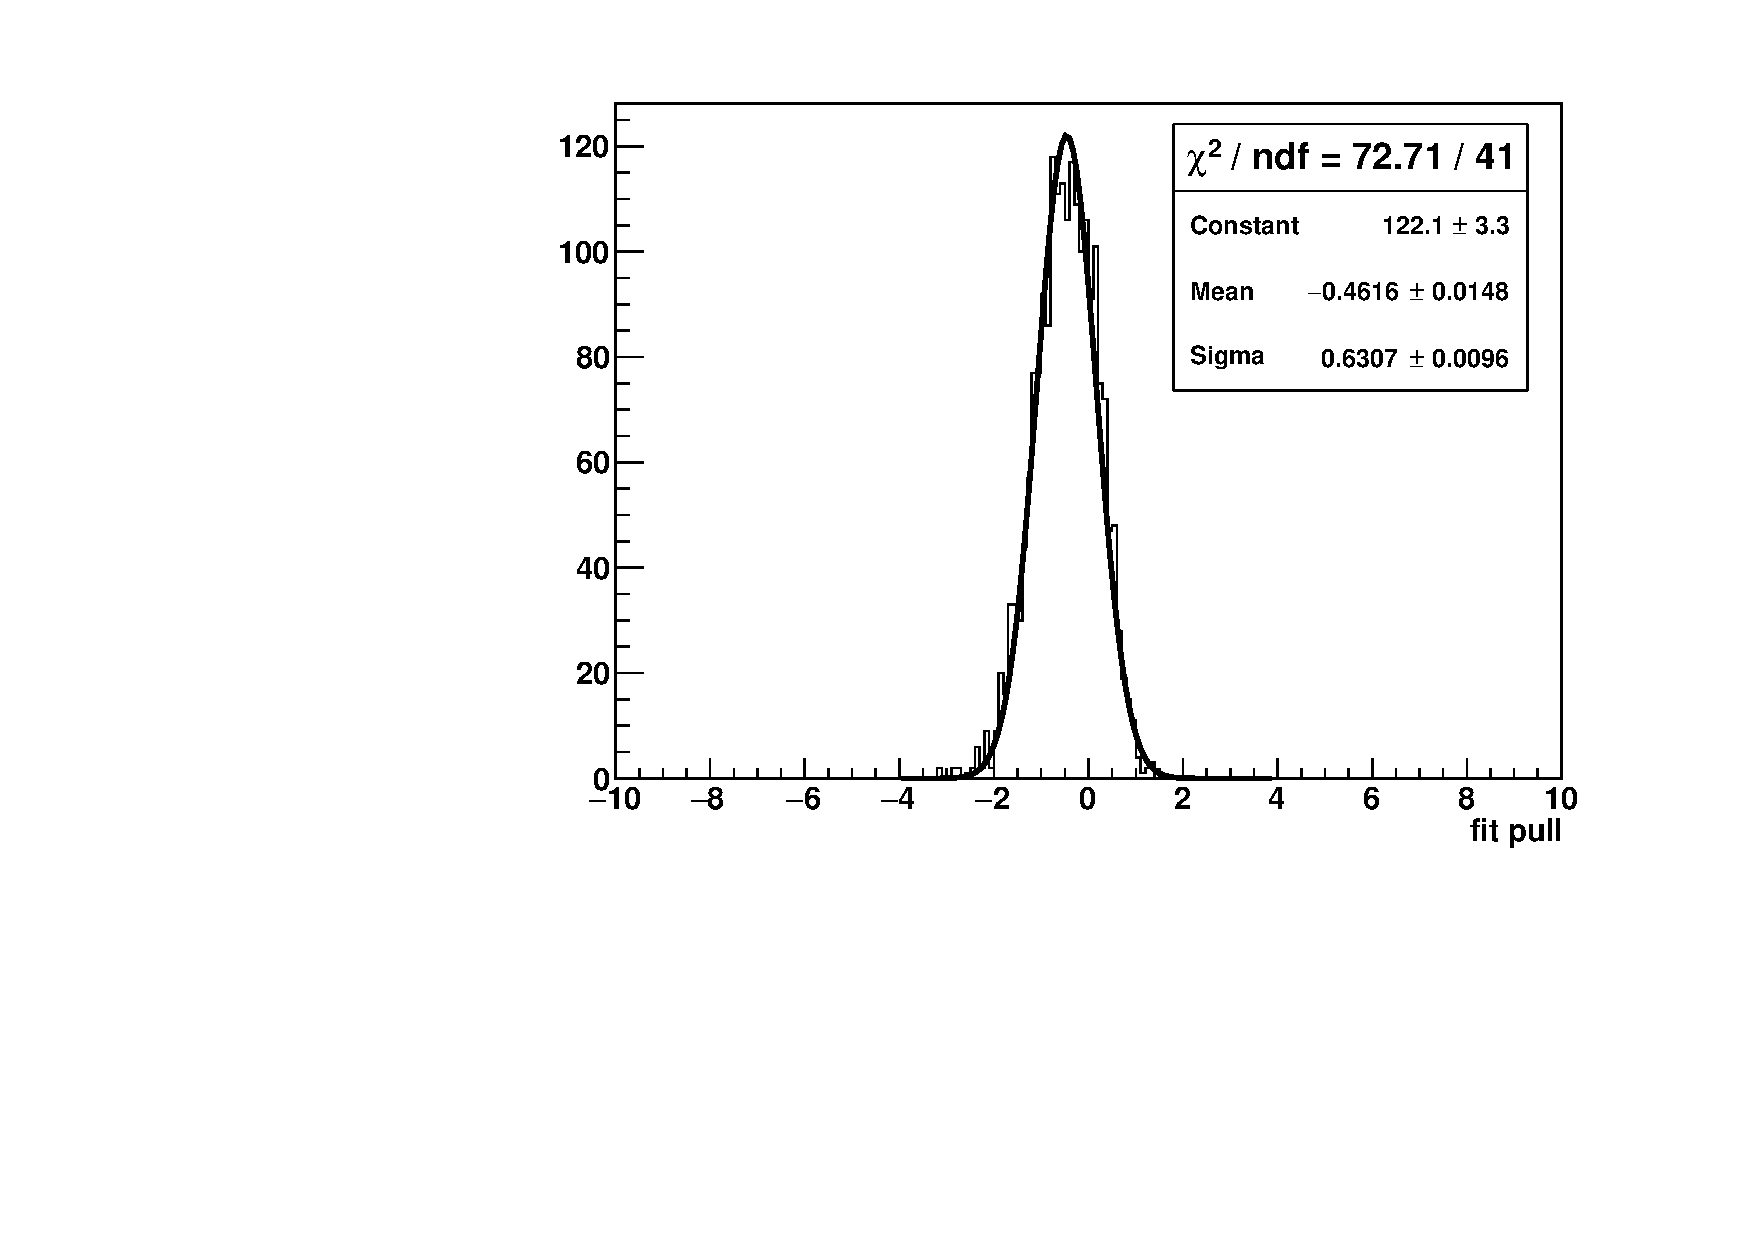
\includegraphics[width=8cm]{ensemble_fitPull.pdf}
	\caption{$N_{sig}$ fit pulls for 5000 fake datasets.}
	\label{poisson_fitPull}
\end{figure} 

\begin{figure}[!htb]
	\centering
	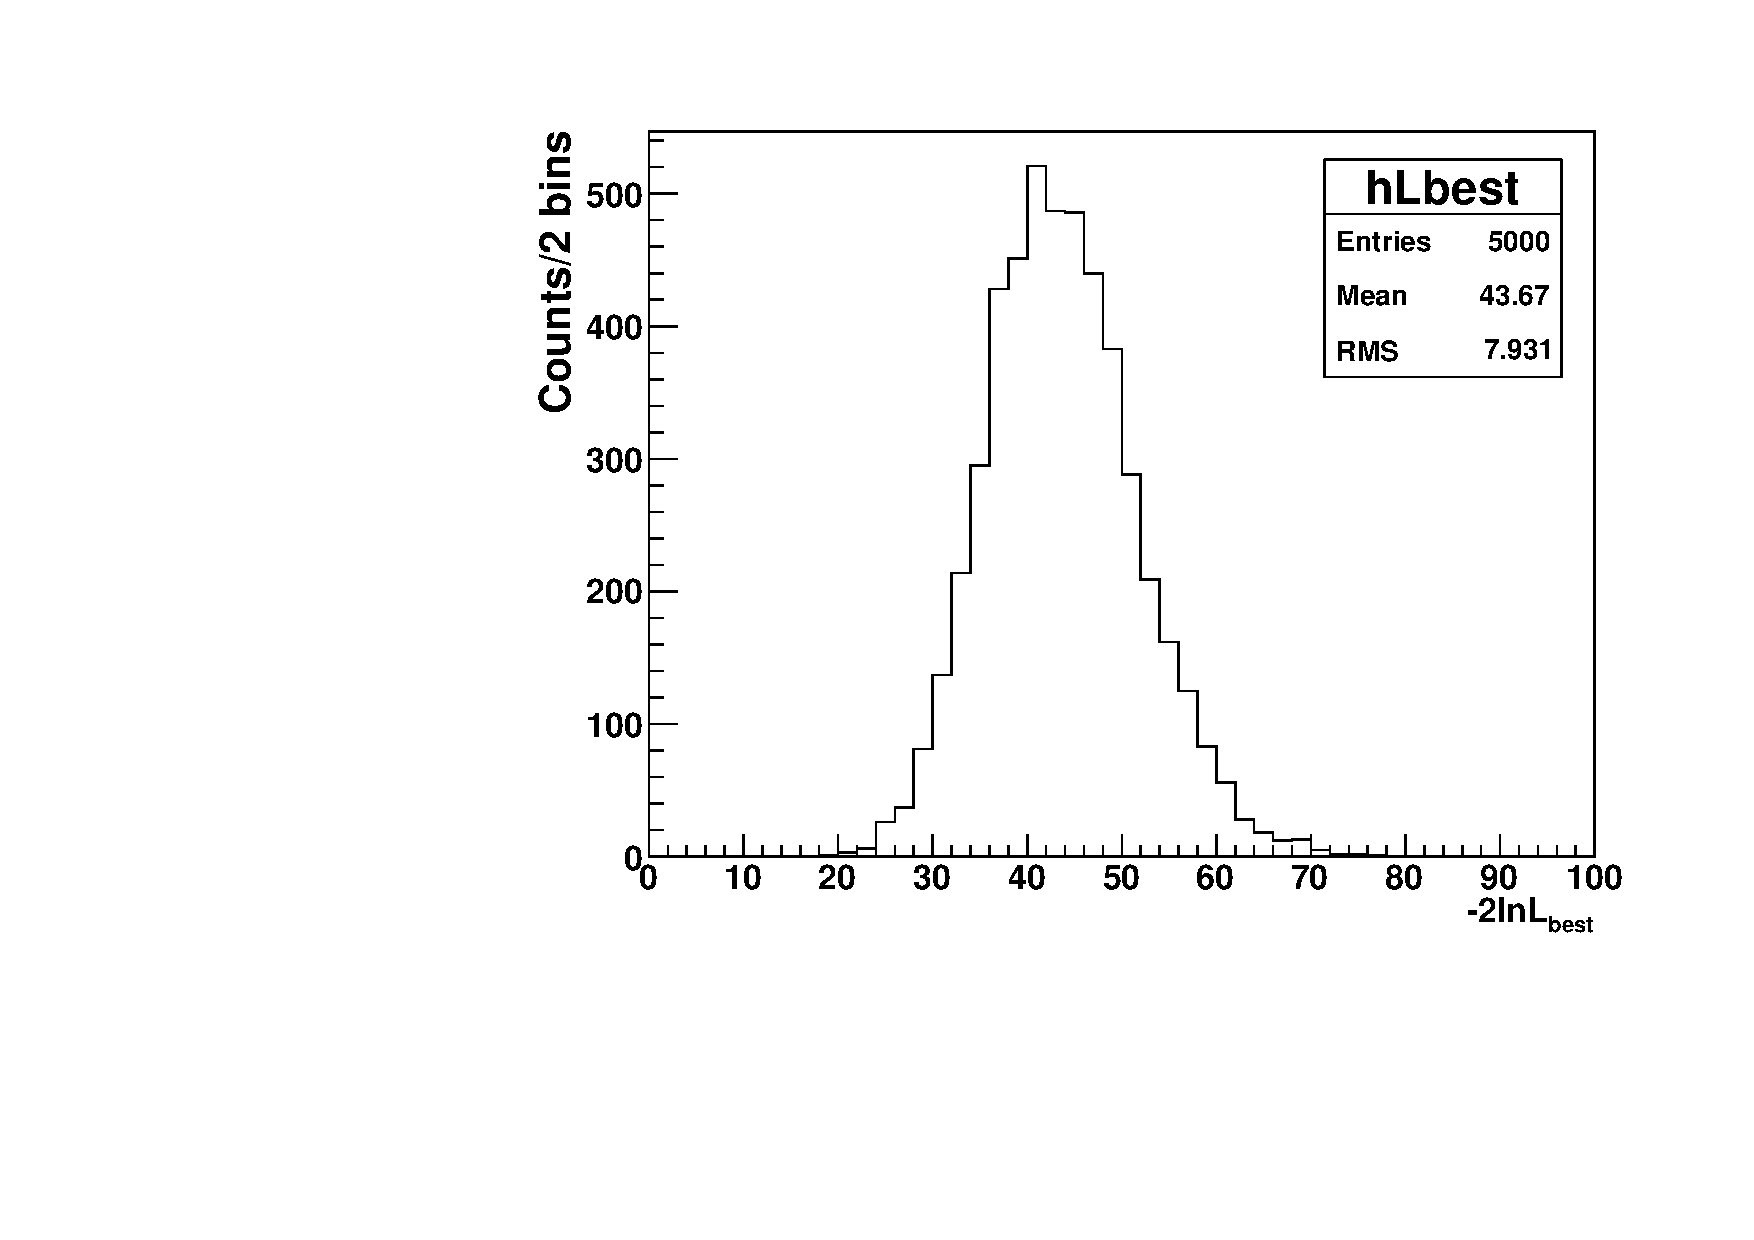
\includegraphics[width=8cm]{ensemble_lnLbest.pdf}
	\caption{The $-2\ln L$ of the best fitted results for 5000 fake datasets.}
	\label{poisson_fitLnL}
\end{figure}

\subsubsection{Fitting on the Whole Dataset (run-200004 to 207718)}
The whole dataset started from run-200004 (on 24 Oct, 2018) to run-207718 (on 10 July, 2019). This dataset has a live time of 190.33 days. The TMAV method was applied to the whole MC datasets of the solar $\nu_e$ simulations as well as the background simulations\footnote{the solar $\nu_mu$ was also trained with the background simulations to calculate the solar neutrino flux mentioned in next section}. The trained BDT and MLP weights were applied to this whole dataset.

In the region of $5<E_{fit}<15$~MeV, the outputs from the BDT and MLP were fitted to obtain the $N_{sig}$ and $N_{bkg}$. Fig.~\ref{wholeDataset_poissonFit_bdt} and Fig.~\ref{wholeDataset_poissonFit_mlp} show their results respectively.

These results are also summarized in Table.~\ref{table:wholedata_output}.

\begin{figure}[!htb]
	\centering
	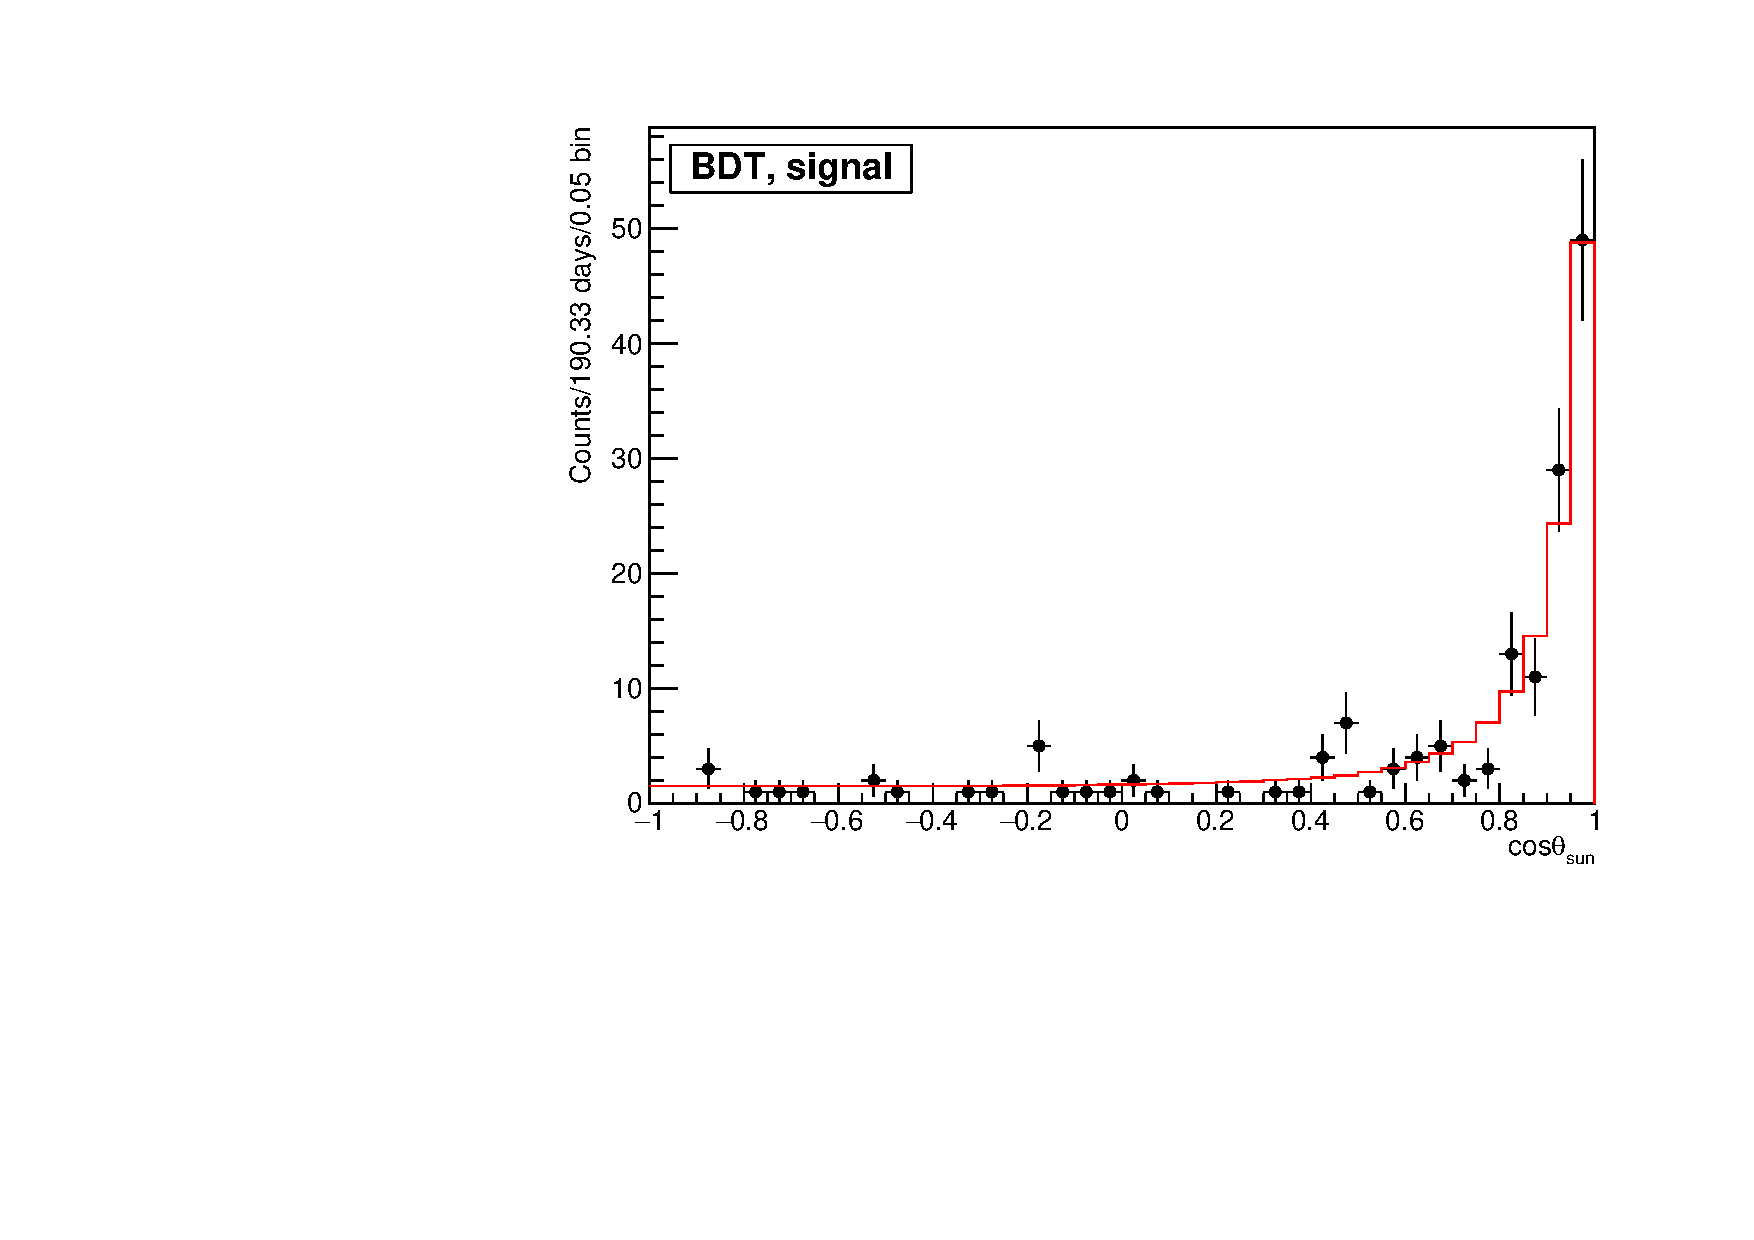
\includegraphics[width=10cm]{wholedataFit_bdt.pdf}
	\caption{Fitted results for the $5<E_{fit}<15$~MeV, from BDT outputs.} \label{wholeDataset_poissonFit_bdt}
\end{figure} 

\begin{figure}[!htb]
	\centering
	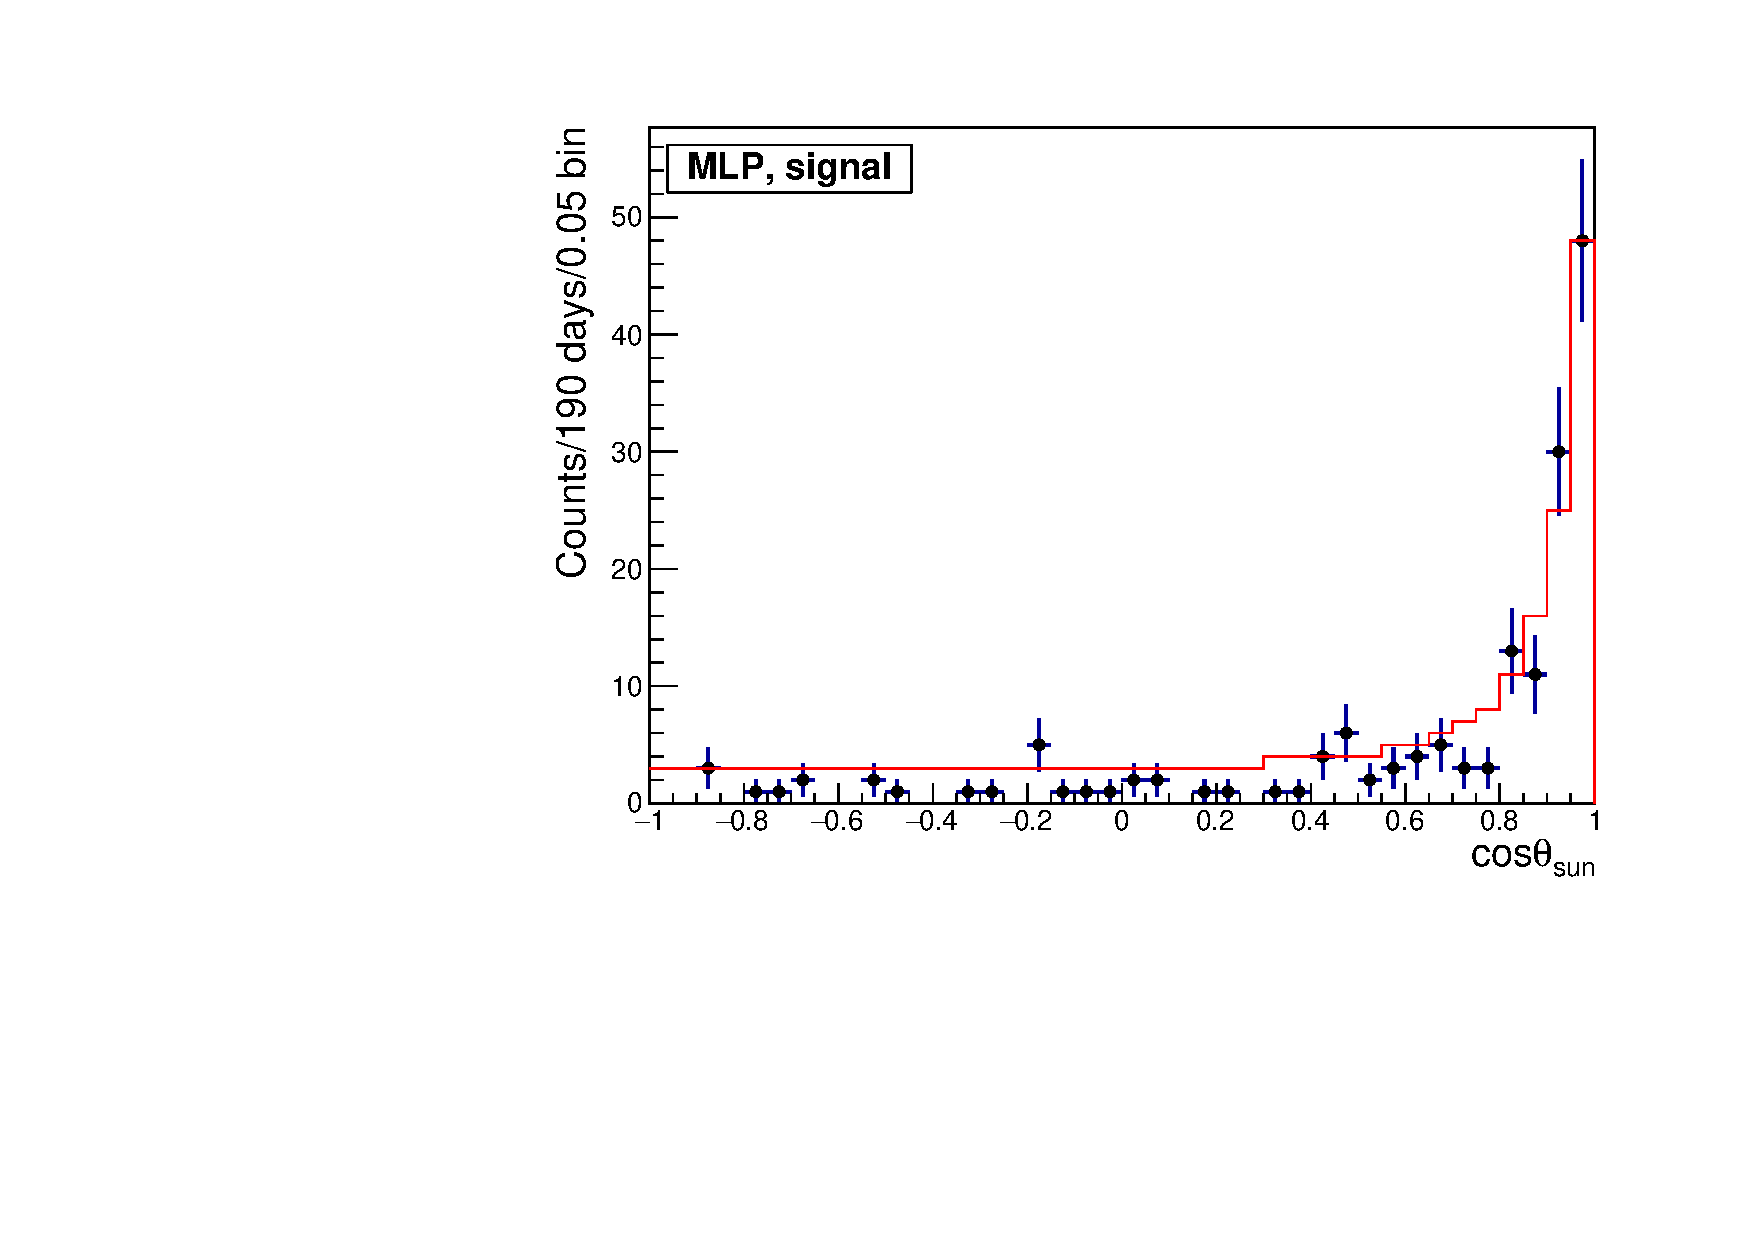
\includegraphics[width=10cm]{wholedataFit_mlp.pdf}
	\caption{Fitted results for the $5<E_{fit}<15$~MeV, from MLP outputs.}
	\label{wholeDataset_poissonFit_mlp}
\end{figure} 

\begin{table}[ht]
	\centering
	\caption{Fitted results for the whole dataset ($5<E<15$~MeV).}
	\label{table:wholedata_output}

	\begin{tabular*}{150mm}{c@{\extracolsep{\fill}}cccccc}
		\toprule
		Methods & $N_{sig}$ & $N_{bkg}$ & $R_{sig}$ & $R_{bkg}$ & p-value \\
		\hline
		BDT &$119.54\pm11.88$ & $38.46
\pm7.75$ & $0.90\pm0.09$ & $0.29\pm0.06$ & 0.14\\
		MLP &$119.02\pm11.84$ & $39.97\pm7.83$ & $0.90\pm0.09$  & $0.30\pm 0.06$  & 0.18\\
		%default cuts& \\ 
		\bottomrule
	\end{tabular*}
\end{table}

It can be concluded here that the BDT results are consistent with the MLP results. The estimated background rate in the [5,15] MeV energy region is about $\frac{1}{3}$ of the signal rate, which indicates that a low background measurement is achieved for the solar neutrino analysis with the energy down to 5 MeV.

\subsubsection{Systematics Evaluation}
In Chapter 5, the reconstruction systematics of position, direction and energy were obtained. The quantities of position scale, position shifts, direction resolution, $\beta_{14}$ shifts, energy scale ($E_{scale}$) and energy resolution ($E_{resol}$) were used to evaluate the systematic uncertainties of the solar neutrino analysis. Table.~\ref{tab:solar_uncertainties} summarizes these systematics and their applications to transform the reconstructed results. In this thesis, only the systematics mentioned below were taken into account, and these systematics are considered uncorrelated. 

\begin{table}[ht]
	\centering
	\caption{Systematics for the solar $\nu_e$ analysis in the water phase.}
	\label{tab:solar_uncertainties}
	\begin{tabular*}{150mm}{c@{\extracolsep{\fill}}ccc}
		\toprule
		Systematics & values (positive/negative) & transformation   \\
		\hline
		x shift ($\Delta x$) & +6.48/-5.98 mm  & $x_{fit}\pm \Delta x$ \\	
		y shift ($\Delta y$)& +6.13/-4.11 mm   & $y_{fit}\pm \Delta y$ \\
		z shift ($\Delta z$)& +6.71/-4.82 mm   & $z_{fit}\pm \Delta z$ \\
		x scale ($\Delta s_x$)& +0.07\%/-0.06\%  & $(1\pm \Delta s_x)x_{fit}$\\	
		y scale ($\Delta s_y$)& +0.02\%/-0.07\%  & $(1\pm \Delta s_y)y_{fit}$ \\
		z scale ($\Delta s_z$)& +0.08\%/-0.01\%  & $(1\pm \Delta s_z)z_{fit}$ \\
	    direction $\delta_\theta$  & +0.013/-0.101 & $1+\frac{\cos\theta_{sun}-1}{1\pm\delta_\theta}$\\
	    $E_{scale}~(\Delta_{\delta_E})$ &  1.0\%  & $(1\pm \Delta_{\delta_E})E_{fit}$\\
	    $E_{resol}~(\Delta_b)$ &  0.037 $\sqrt{\mathrm{MeV}}$  & $E_{fit}+Gaus(0,\sigma_{smear})$, \\
	    & &$\sigma_{smear}=\sqrt{E_{fit}}\sqrt{(1+\Delta_b)^2-1}$\\
	    $\beta_{14}$ shift ($\Delta \beta_{14}$) & +0.010/-0.036 & $\beta_{14}\pm \Delta \beta_{14}$\\
		\bottomrule
	\end{tabular*}
\end{table}

Note that the position shifts were applied to the $x_{fit},~y_{fit}$, and $z_{fit}$ respectively, while the position scales were applied simultaneously to the position vector: 

$\vec{X'}_{fit}=((1\pm \Delta s_x)x_{fit},(1\pm \Delta s_y)y_{fit},(1\pm \Delta s_z)z_{fit})$.

To evaluate the systematics of the solar neutrino analysis, the systematic transformations in Table.~\ref{tab:solar_uncertainties} were applied to the reconstructed quantities in MC simulations independently. The reconstructed quantities after the transformations are called ``smeared'' values. The smeared values of an event can affect whether the event will pass the cuts: the smeared positions of an event affect whether the event can pass the fiducial volume cut and then affect the results after the position cuts; the smeared energies affect the results after the energy cuts and the smeared $\beta_{14}$ affect the results after the $\beta_{14}$ cuts. Thus, for the solar $\nu_e$ and $\nu_\mu$ simulations, the shape of the $\cos\theta_{sun}$ distribution used as the $PDF$ will be changed by the smeared values. In addition, the $\delta_\theta$ transformation changes the $PDF$ shape directly. Finally, the spectrum from the data was re-fit with the smeared $PDF$s to obtain the physics quantity (specifically, the flux ratio mentioned in the next section), and the different fit results are used as the systematics of the physics quantity.

To obtain the smeared $PDF$s, first, the ``beforehand cut'' mentioned before was loosen by removing the cuts on $\beta_{14}$ and $R'_{fit}$ (fiducial volume), and only the cuts NHit$>20$ (reconstruction threshold) and $ITR>0.55$ (determined from the instrumental noises and its systematic uncertainty was not considered) were applied to the MC simulations of the solar $\nu_e$ and $\nu_\mu$. Then the systematic transformations were applied one by one and event by event. The positive (``smearing up'') and negative (``smearing down'') values were also applied, respectively. After the transformation, the whole ``beforehand cut'' was applied. At last, the TMVA BDT selection was applied. For a specific smeared quantity, the final output of the MC $\cos\theta_{sun}$ spectrum was used as the smeared $PDF$ for that quantity. For example, if the $E_{fit}$ is smeared by scaling up: $E_{fit}=(1+\Delta_{\delta_E})E_{fit}$, then outputs of the $\cos\theta_{sun}$ after the ``beforehand cut'' and TMVA BDT selection is used as the ``energy scale-up $PDF$''.
 
\subsubsection{Evaluating $^8$B Solar Neutrino Flux}

A software called \texttt{PSelmaa} (Physics interpretation Sun-Earth Large Mixing Angle Adiabatic
Approximation) was implemented in \texttt{RAT}\cite{fady_pselmaa}. The software uses the BS05(OP) SSM model. It assumes the normal mass hierarchy. It also applies the MSW effects from the Sun (see Chapter 2) but neglects the MSW effects from the Earth (i.e., the regeneration of coherence in the Earth). Fig.~\ref{fig:pselmaa_curves} shows the survival probability curve as a function of energies (in 0.1 MeV intervals) taken from the \texttt{PSelmaa}.

Since SNO+ can not discriminate $\nu_\mu$ and $\nu_\tau$, only the $\nu_\mu$ MC is included in the $P_{e\alpha}$.

\begin{figure}[!htb]
	\centering
	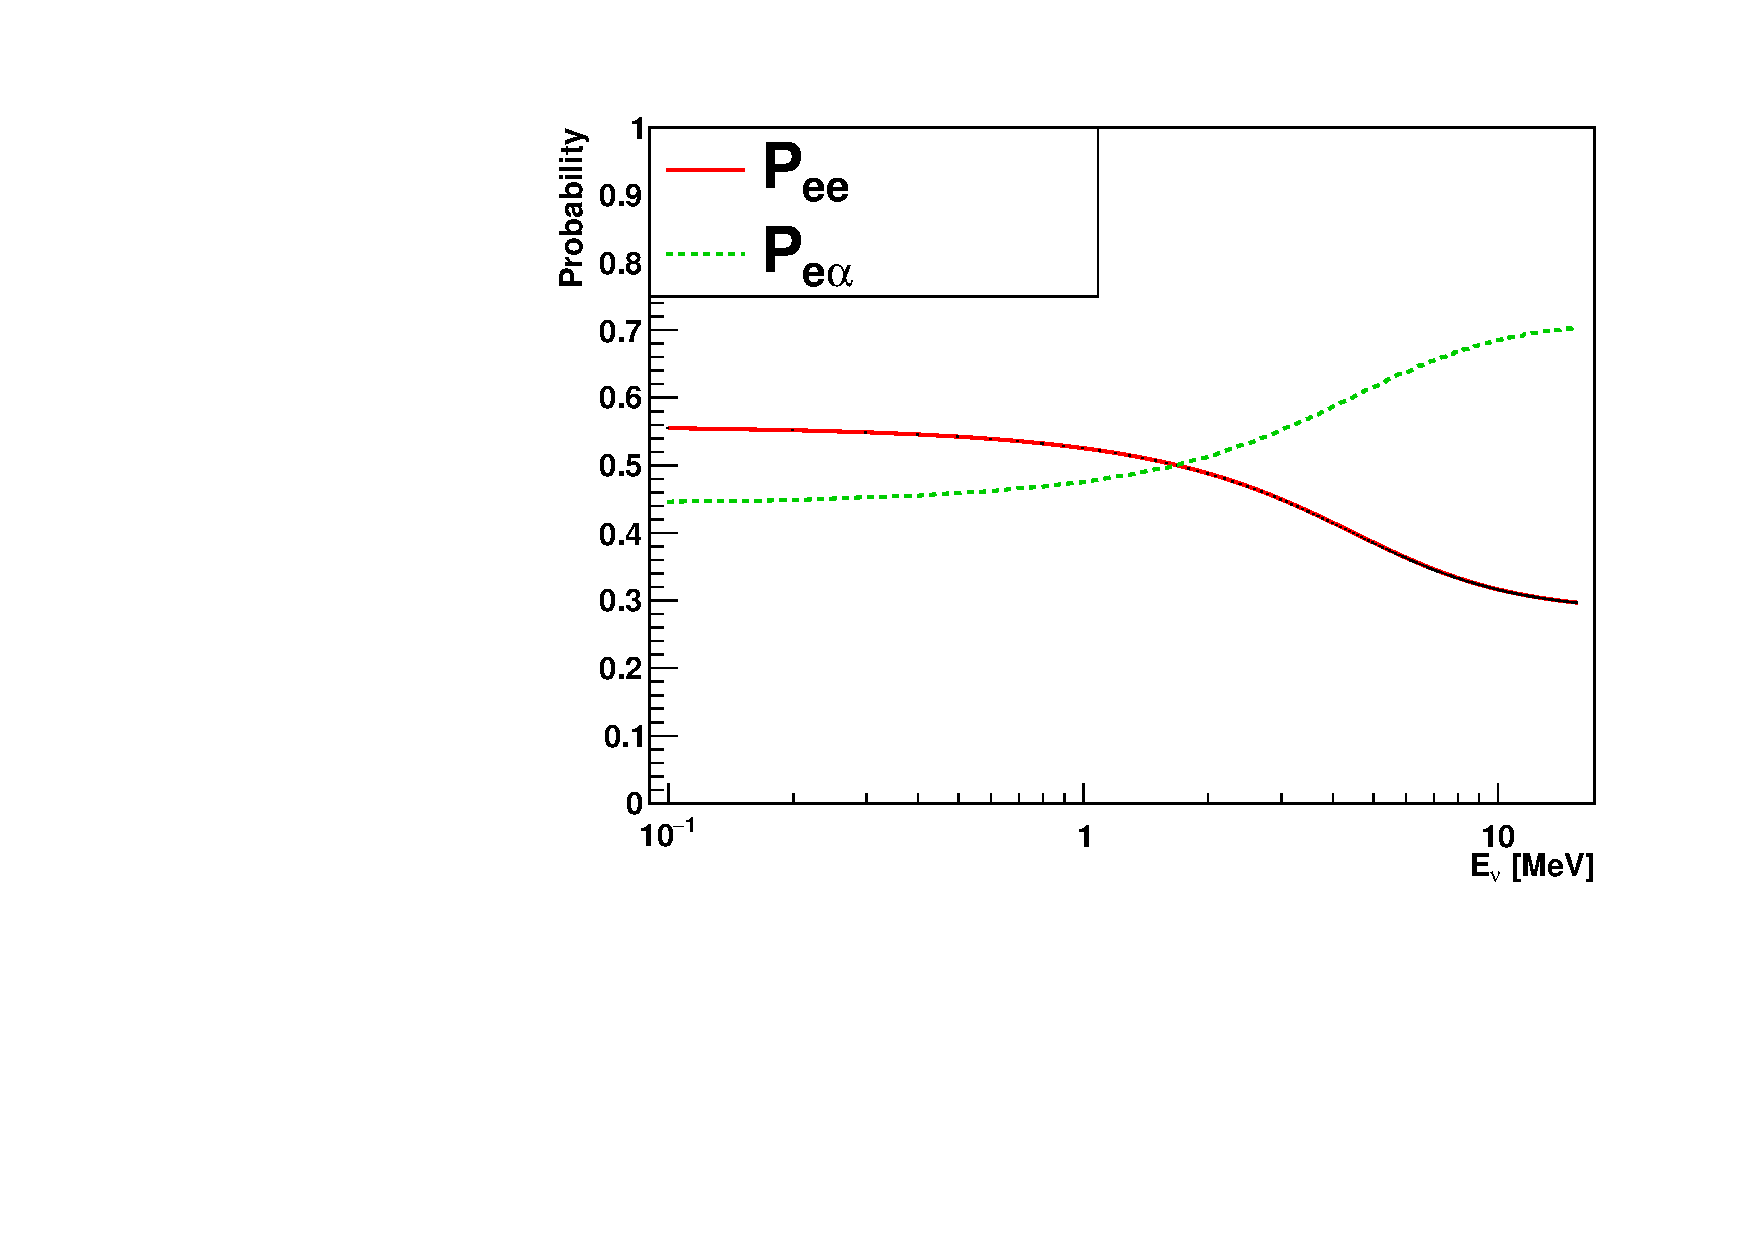
\includegraphics[width=10cm]{PSelmaa_bs05op.pdf}
	\caption[The MSW survival probability curves as functions of MC energies.]{The MSW survival probability curves as functions of MC energies. The $P_{ee}$ is in solid red line and $P_{e\alpha}(=1-P_{ee})$ is in green dashed line.}
	\label{fig:pselmaa_curves}
\end{figure}

%To evaluate the $^8$B solar neutrino flux, the fitted number of $\nu e^-$ elastic scattering (ES) is divided by the expected number of ES and is then multiplied by the flux in the MC: 
%\begin{equation}
%\Phi_{^8B} = \Phi_{^8B,MC}\frac{N_{fit}}{N_{expected}},
%\end{equation}

To gain more statistics of the MC simulations, the number of the simulated solar $\nu_e$ events is 1700 times the nominal ($flux~scale = \frac{1}{1700}$); while the number of the solar $\nu_\mu$ events is 9600 times the nominal($flux~scale=\frac{1}{9600}$). Since it is impossible for the SNO+ detector to discriminate between $\nu_\mu$ and $\nu_\tau$ via detecting the elastic scattering events, $\nu_\tau$ is not generated separately. Therefore, the generated solar $\nu_\mu$ events are considered as a combination of $\nu_\mu$ and $\nu_\tau$ ($\nu_\mu\approx\nu_{\mu,\tau}$) in the solar neutrino flux. In addition, to compare the MC with the data, a live time scale was taken into accounts: $t_{frac}=\frac{t_{data~live~time}}{t_{MC~run~time}}=\frac{190.33~days}{198.17~days} = 0.96$.

a dataClean cut of 1.7\% was assumed here.

Therefore, the numbers of the MC generated $\nu_e$ and $\nu_\mu$ events are scaled by the $t_{frac}$ and $flux~scale$, and then weighted by the oscillation probability $P_{ee}$ and $P_{e\alpha}=1-P_{ee}$. Applying these weighting parameters as well as the BDT cuts to the MC histograms, the MC $\cos\theta_{sun}$ distributions in the energy region $5<E_{fit}<15$ MeV with and without oscillations are shown in Fig.~\ref{fig:MCfluxPdfs}.

\begin{figure}[!htb]
	\centering
	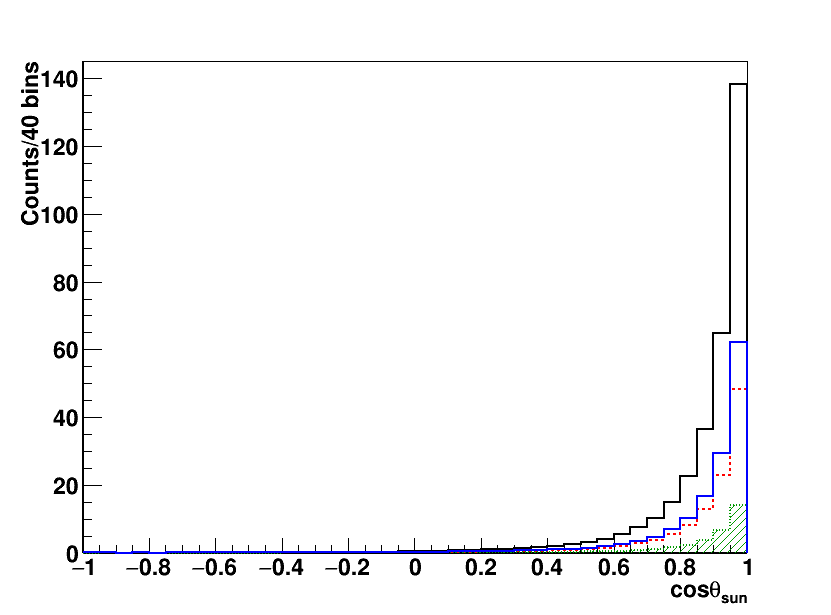
\includegraphics[width=8cm]{MCfluxPdfs.png}
	\caption[The MC $\cos\theta_{sun}$ distributions used as $PDF$s for the flux calculations, for $5<E_{fit}<15$ MeV after the BDT cuts.]{The MC $\cos\theta_{sun}$ distributions used as $PDF$s for the flux calculations, for $5<E_{fit}<15$ MeV after the BDT cuts. The histogram in black is the $\nu_e$ flux without oscillation, denoted by $PDF(\nu_e,without~oscillation)$. This histogram is used for fitting the elastic scattering flux. The dashed red histogram is the $\nu_e$ flux and the dashed green shaded histogram is the $\nu_\mu$ flux, both including the oscillation. These two histograms were combined to form the blue histogram as the total flux including the oscillation, denoted by $PDF(\nu_e+\nu_\mu,oscillated)$, which is used for fitting the total flux.}
	\label{fig:MCfluxPdfs}
\end{figure} 

Reading from the above histograms, the expected event number for $\nu_e$ without the oscillation is $N_{\nu_e} = 322.69$ while including the oscillations, the expected event number for $\nu_e$ and $\nu_\mu$ are $N^{osci}_{\nu_e} = 113.58$ and $N^{osci}_{\nu_\mu} = 32.64$ respectively, and the combined event number is $N^{osci}_{\nu_e+\nu_\mu}=146.22$.

To fit for the total $^8$B neutrino flux, the fit parameter used here is the flux scale $f_s$, which is interpreted as the fraction of the observed $^8$B flux to the expected flux. Using the same method in Sect.~\ref{sect:poisson_fit}, and in the Eqn.~\ref{eq:solar_poissonFitMinimizer}, replacing the $N_{sig}$ with $N_{sig}=f_s\cdot N^{osci}_{\nu_e+\nu_\mu}(=146.22)$, and then fitting the $N_{sig}$ and the $N_{bkg}$ with the $pdf(\nu_e+\nu_\mu,oscillated)$. The fit results are $f_s=0.82\pm 0.08$ (corresponding to $N_{sig}=119.35\pm11.70$  events) and $N_{bkg}=36.64\pm7.55$ events, with a p-value of 0.0714. The fit result is shown in Fig.~\ref{fig:TOTALfluxFit}.

\begin{figure}[!htb]
	\centering
	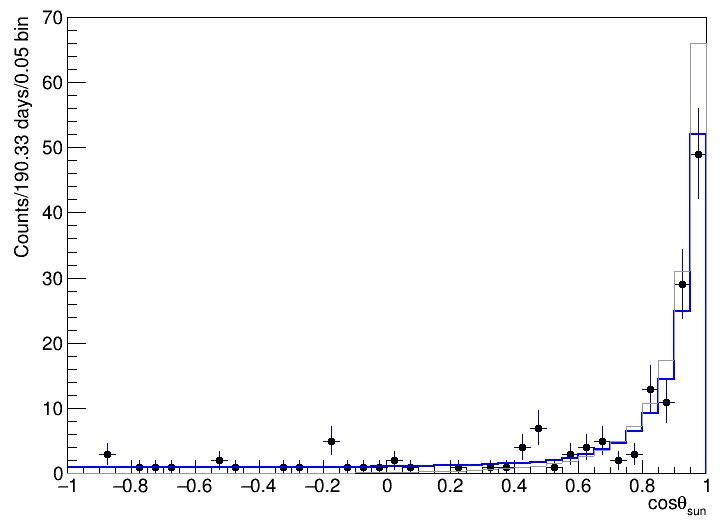
\includegraphics[width=8cm]{TOTALfluxFit.png}
	\caption[A fit on the total $^8$B flux.]{A fit on the total $^8$B flux. The gray histogram is the $PDF(\nu_e+\nu_\mu,with~oscillations)$, the distribution of $\nu_e$ flux without oscillation. The black dots are the data points and the blue histogram is the fitted ES flux.}
	\label{fig:TOTALfluxFit}
\end{figure}

Thus, with the nominal $^8$B solar neutrino flux $\Phi^{total}_{MC}=5.46\times 10^6~cm^{-2}s^{-1}$, the estimated total flux here is:

\begin{equation}
\mathrm{\Phi^{total}_{fit}(^8 B)=f_s\cdot \Phi^{total}_{MC}=(
 4.93 \pm 0.49(stats.))\times 10^6~cm^{-2}s^{-1}}.
\end{equation}

Applying the same systematics in Table.~\ref{tab:solar_uncertainties} to the MC ES $PDF$, and then refit the data with the smeared $PDF$, the smeared values of the flux ratio ($f'_s$) were found. The systematics of the $f_s$ are calculated by $\Delta f_s =f'_s-f_s$. It finds that the position and $\beta_{14}$ smearing are negligible while the direction and energy smearing give more obvious uncertainties. These results are listed in Table.~\ref{tab:smearingResults}. Fig.~\ref{smearESpdfs} shows the effects of smearing the energy resolution and direction on the MC $PDF$. The original MC $PDF$ is shown as black solid line histograms, overlaid by the smeared histograms. 

\begin{table}[ht]
	\centering
	\caption{Systematics for the fitted flux scale $f_s$.}
	\label{tab:smearingResults}
	\begin{tabular*}{80mm}{c@{\extracolsep{\fill}}cc}
		\toprule
		Systematics & $\Delta f_s$ (+/-)\\
		\hline
		x shift & $+0.000003/-0.000045$\\	
		y shift & $+0.000009/-0.000056$\\
		z shift & $+0.0001/-0.000138$\\
		position scale & $+0.00132/-0.00115$\\\	
		$\delta_\theta$  &$+0.01858/-0.002112$\\		
		$E_{scale}~(\Delta_{\delta_E})$ & $+0.01466/-0.01395$\\
		$E_{resol}~(\Delta_b)$ & $+0.0428/-0.0428$ \\
		$\beta_{14}$ shifts & $+0.000178/-0.000558$\\
		\bottomrule
	\end{tabular*}
\end{table}

\begin{figure}[htbp]
	\centering
	\subfigure[Smearing direction parameter $\delta_\theta$. The histogram with black solid line is the original. The blue dotted histogram is for smearing down and the red dashed is for smearing up.]{ 
		\begin{minipage}[t]{0.5\textwidth}
			\centering
			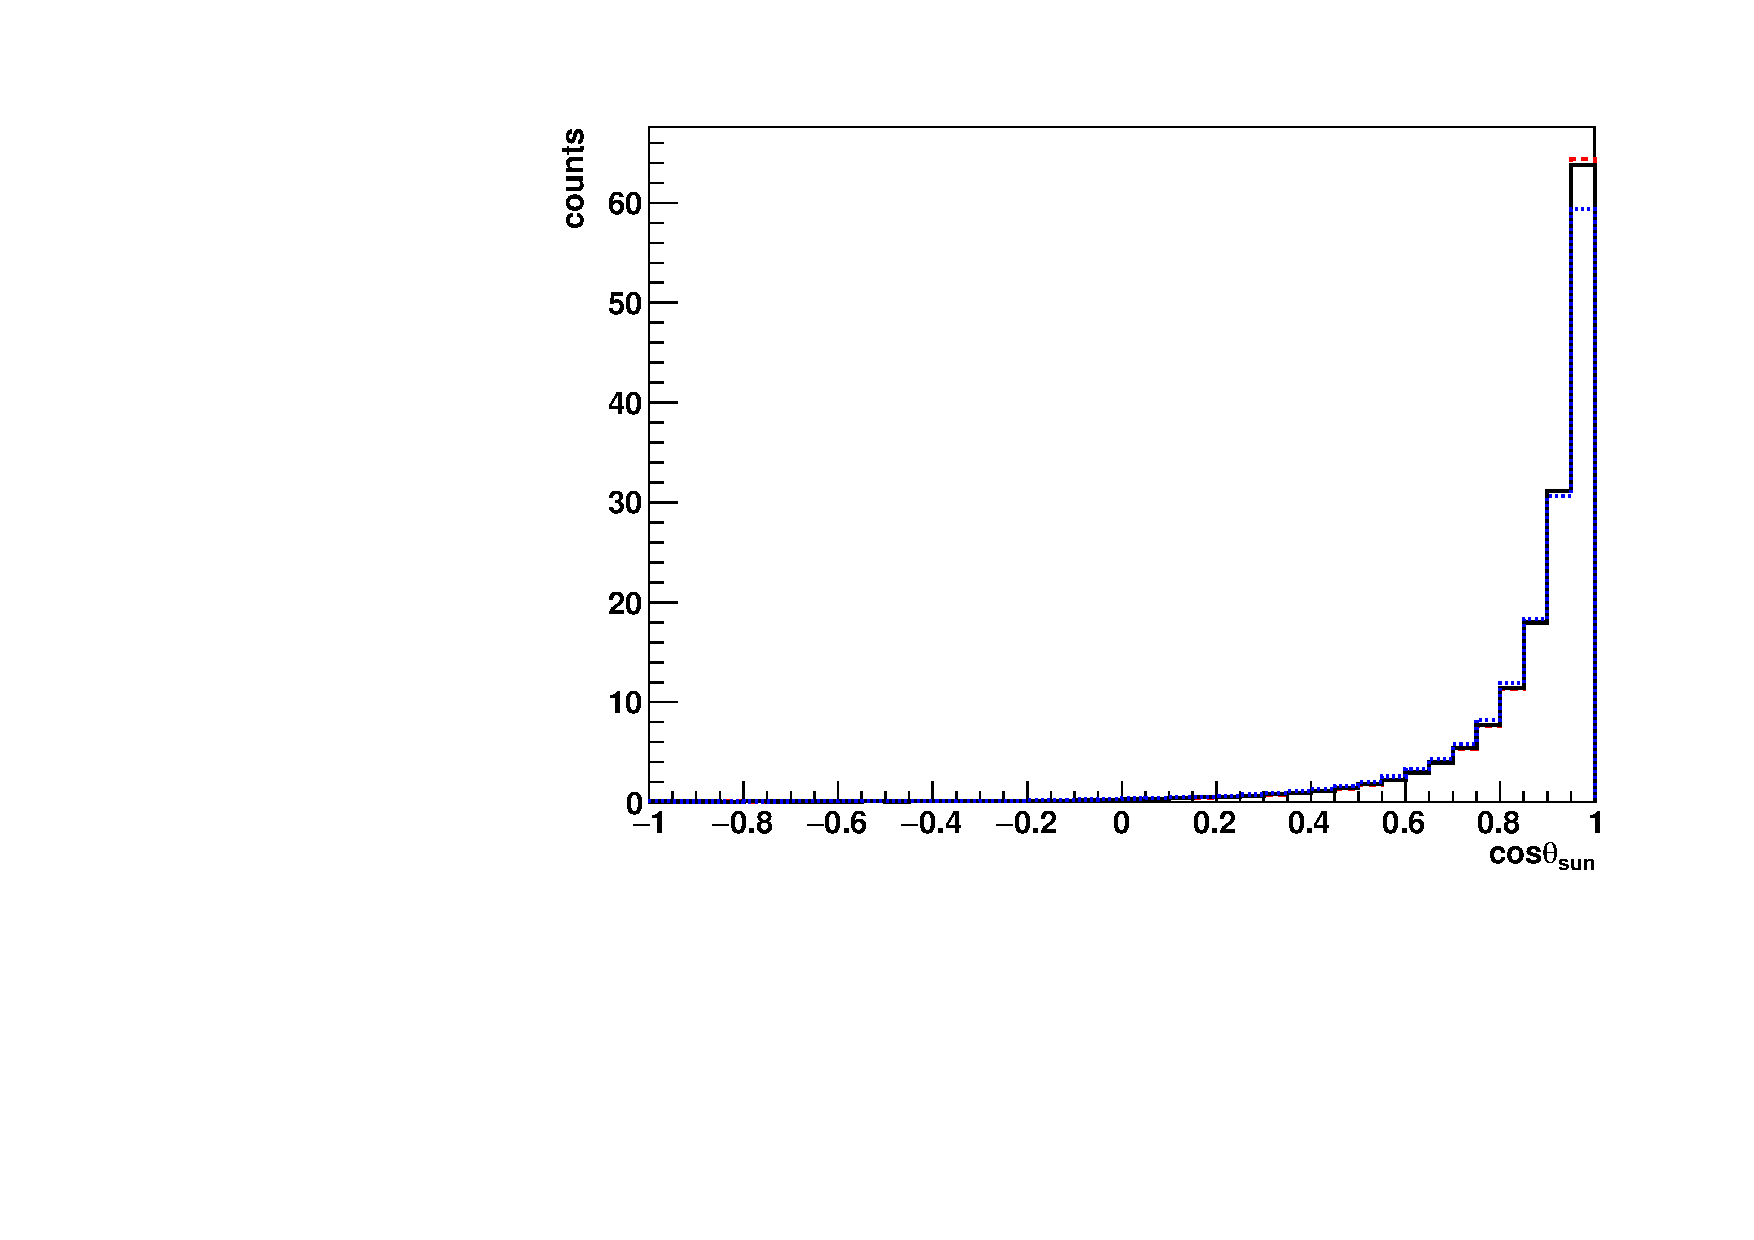
\includegraphics[width=8cm]{smearCosSunPDF_Dir.pdf}
		\end{minipage}
	}
	\subfigure[Smearing energy resolution. Red dashed line for smearing down the $E_{resol}$.]{ 
		\begin{minipage}[b]{0.5\textwidth}
			\centering
			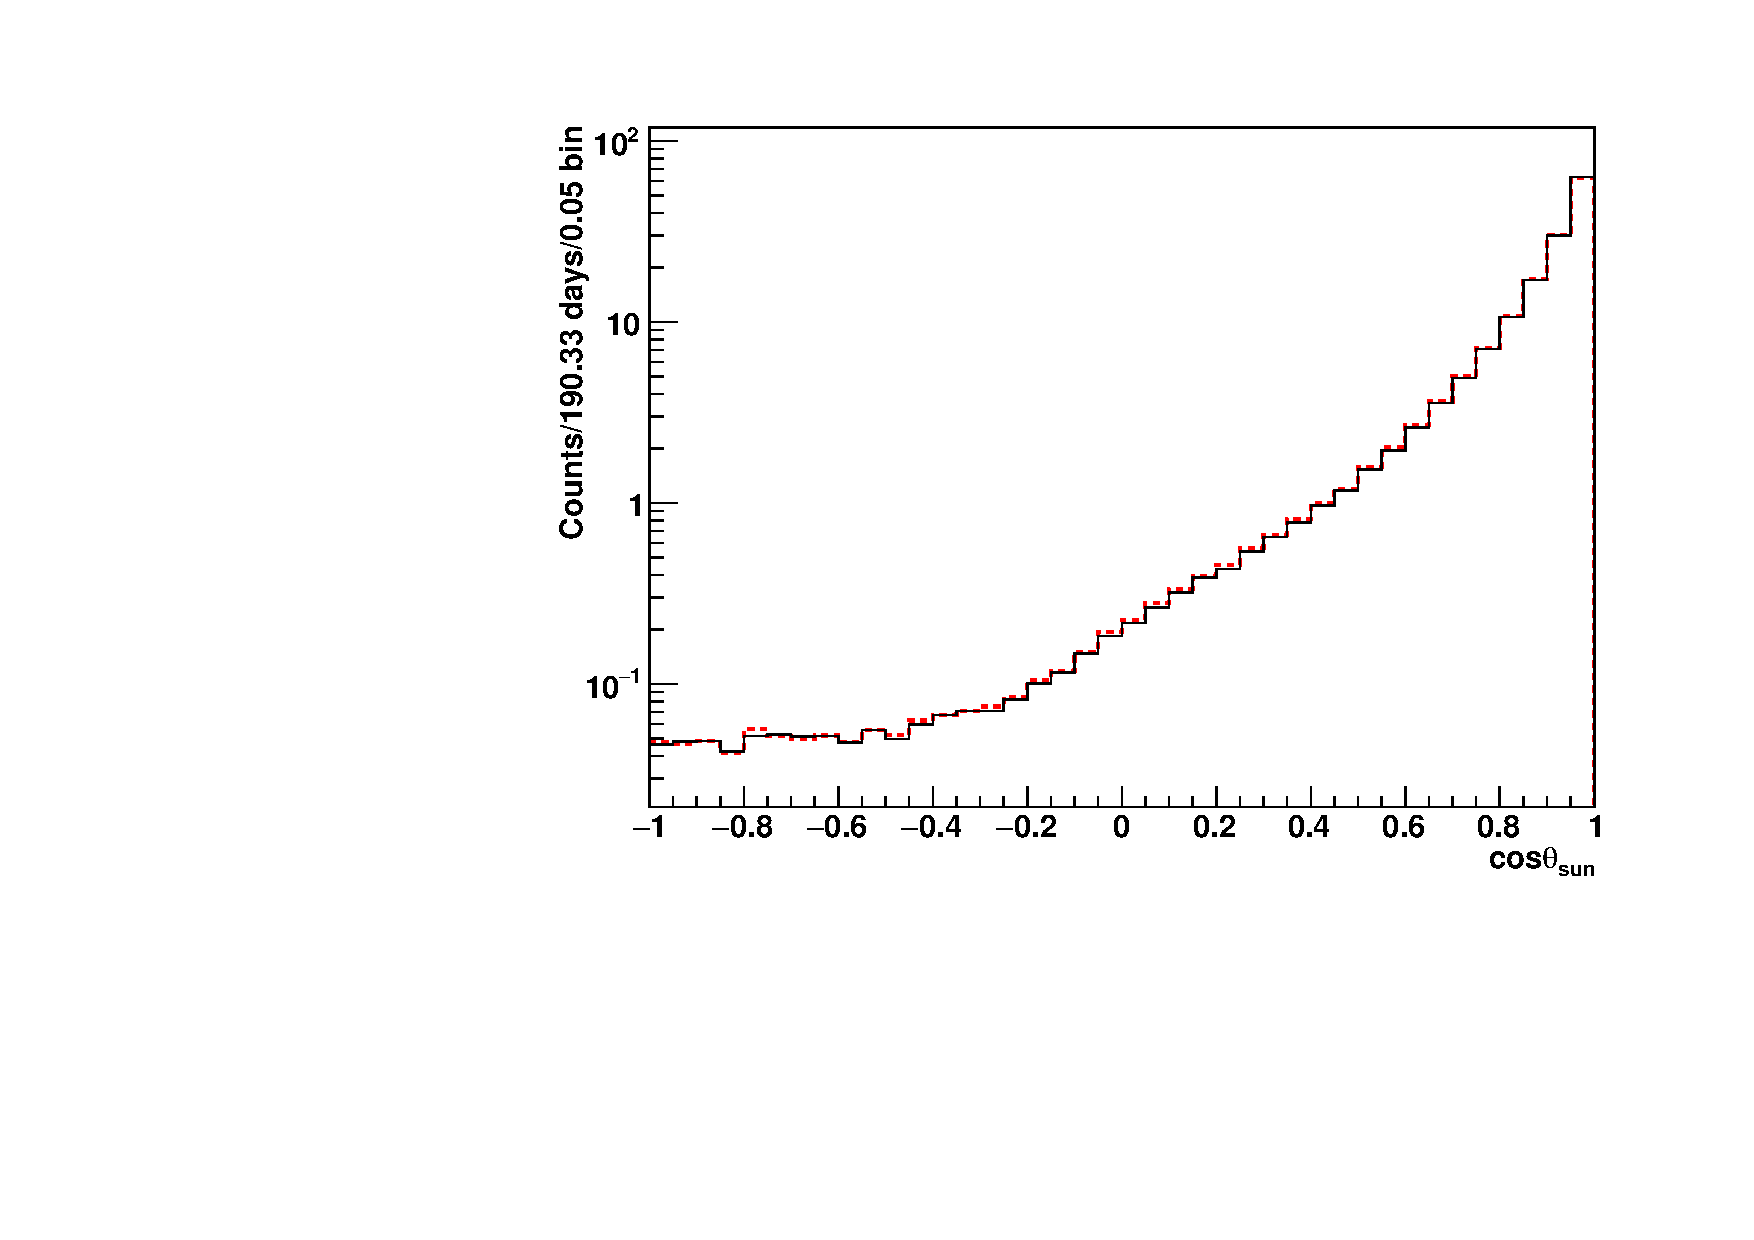
\includegraphics[width=8cm]{smearCosSunPDF_Eresol.pdf}
		\end{minipage}
	}
%	\subfigure[Smearing energy scale. The histogram with black solid line is the original. The blue dotted histogram is for smearing down and the red dashed is for smearing up.]{ 
%		\begin{minipage}[t]{0.4\textwidth}
%			\centering
%			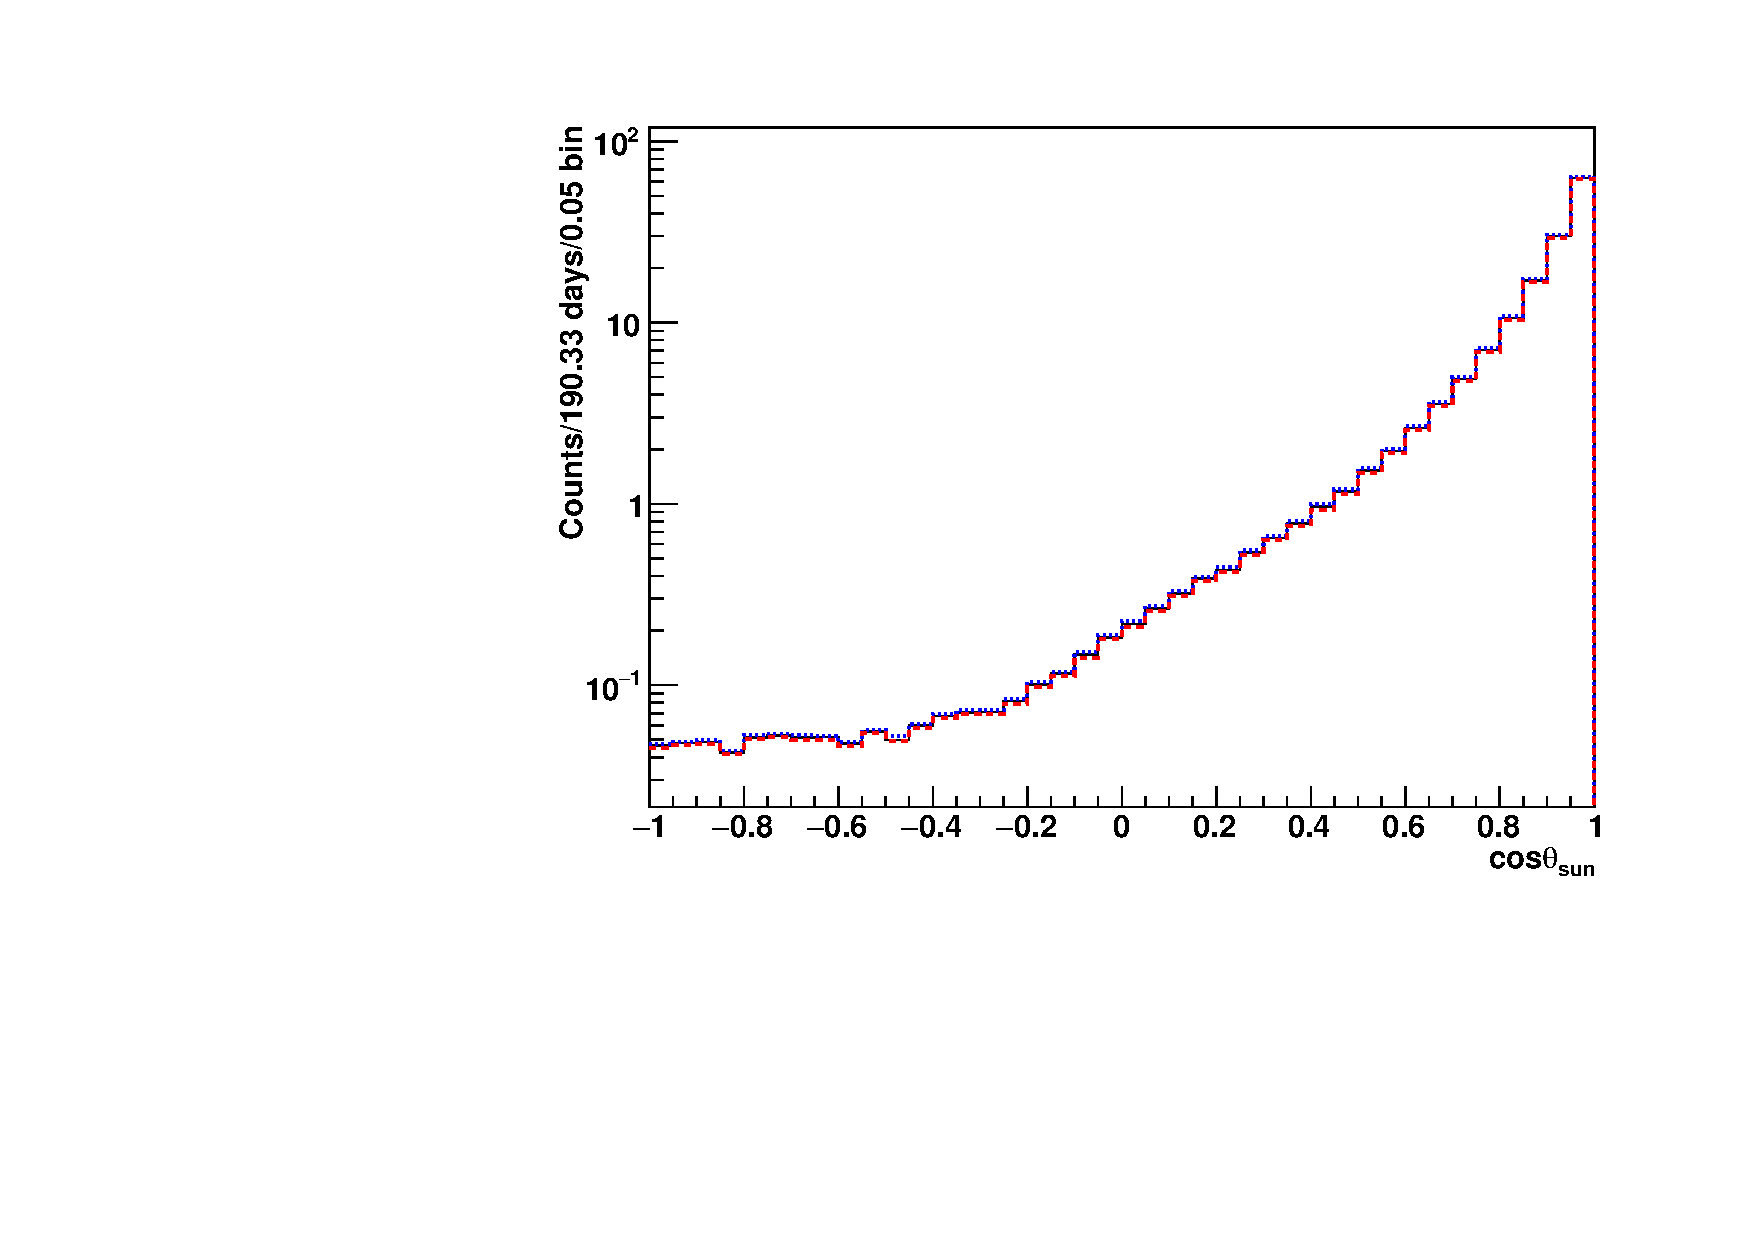
\includegraphics[width=8cm]{smearCosSunPDF_Escale.pdf}
%		\end{minipage}
%	}
	\caption[Smearing effects on the $\cos\theta_{sun}$.]{Smearing effects on the $\cos\theta_{sun}$.	\label{smearESpdfs}}
\end{figure}   

Using the quadrature sum assuming all the variables are independent, the total systematics is expected to be: ${f_s}^{+0.0240}_{-0.0142}$. Adding these systematics, the total flux is:
\begin{equation}
\mathrm{\Phi^{total}_{fit}({^8 B})=f_s\cdot \Phi^{total}_{MC}=(4.48\pm 0.44(stats.)^{+0.13}_{-0.08}(syst.))\times 10^6~cm^{-2}s^{-1}.}
\end{equation}

To fit for the $^8$B flux corresponding to an observed flux of ES interactions, the same procedure was used, while the fit parameter was changed to $N_{sig}=f_s\cdot N_{\nu_e}(=314.68)$ and the $PDF$ was changed to $PDF(\nu_e,without~oscillation)$. As shown in Fig.~\ref{fig:ESfluxFit}, the fit results are $f_s=0.3798\pm 0.03772$ (corresponding to $N_{sig}=119.52\pm11.62$ events) and $N_{bkg}=36.81\pm 7.56$ events, with a p-value = 0.14.

\begin{figure}[!htb]
	\centering
	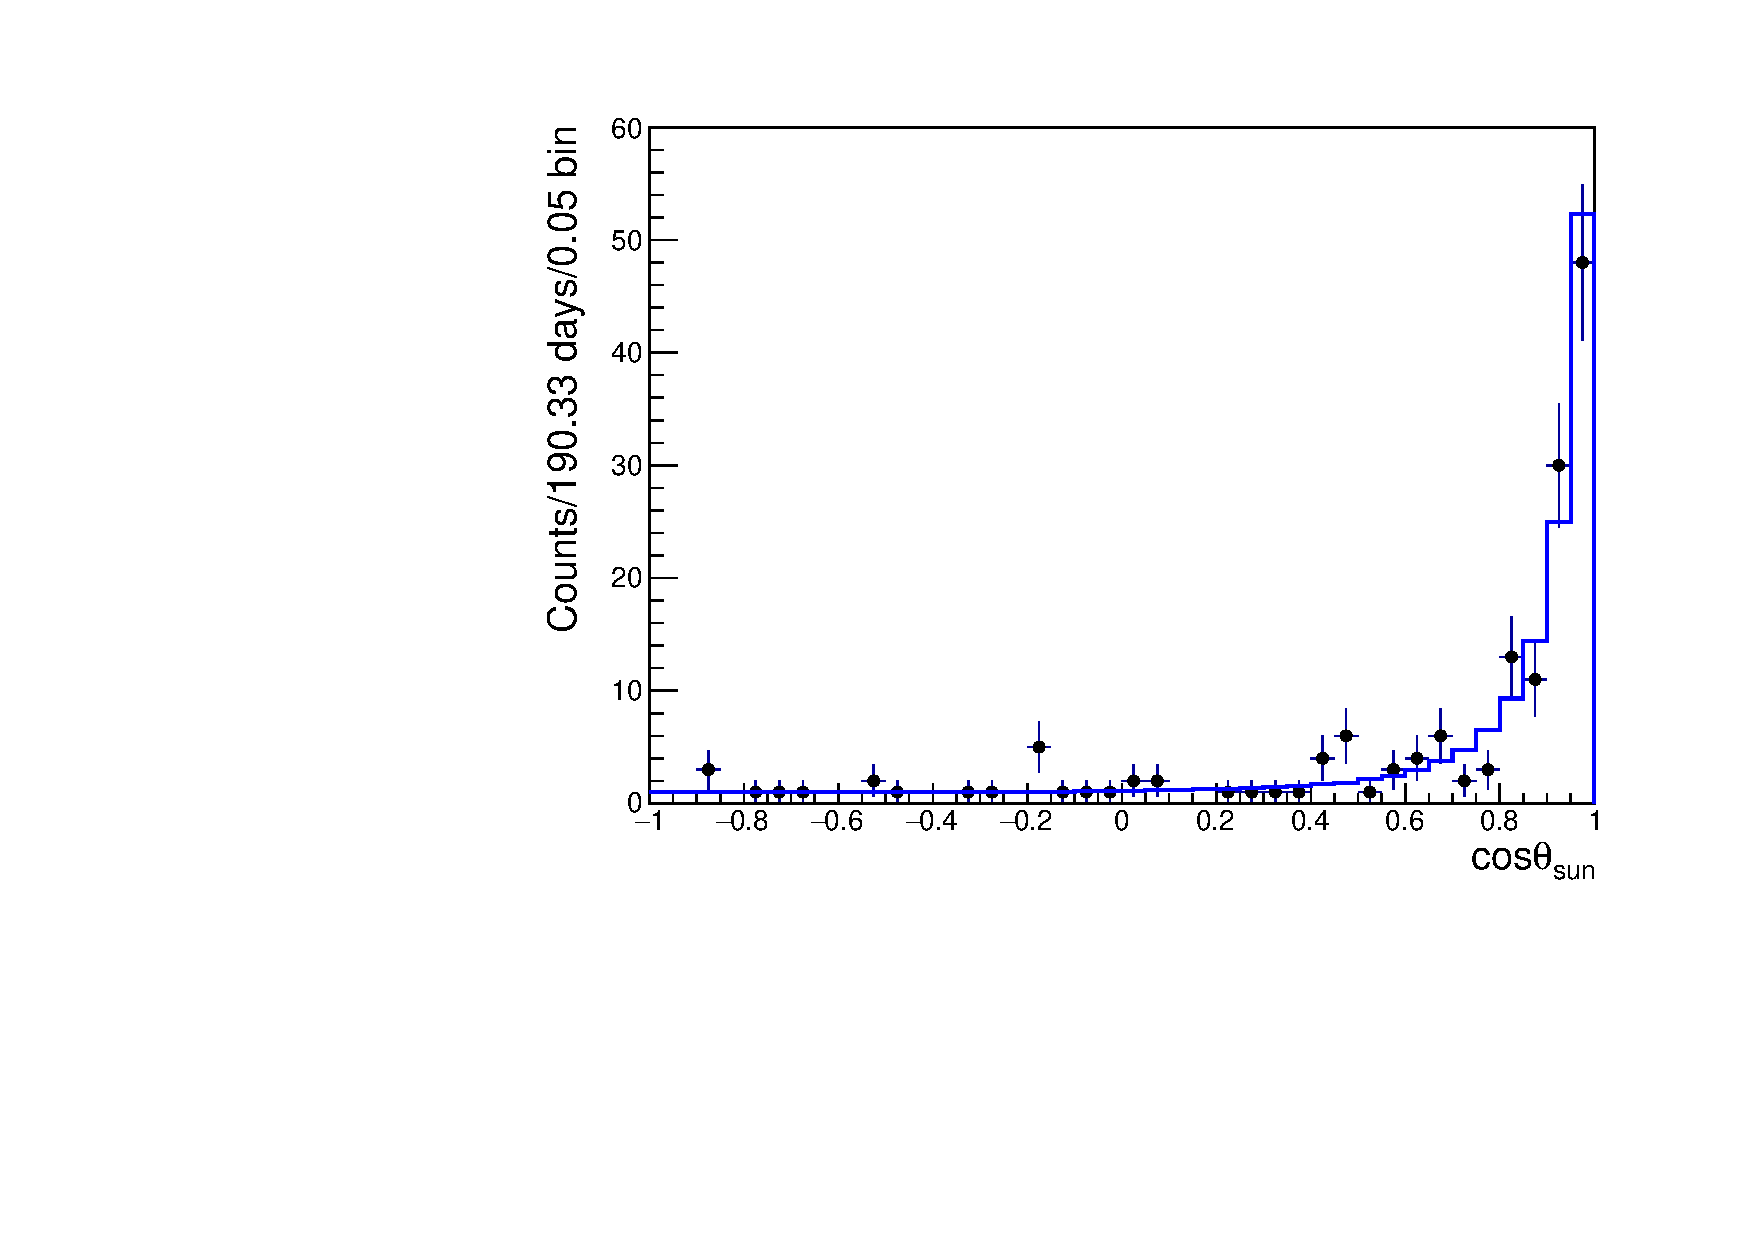
\includegraphics[width=10cm]{ESfluxFit.pdf}
	\caption[Fitting with the spectrum of elastic scattering.]{Fitting with the spectrum of elastic scattering. The gray dotted histogram is the distribution of $\nu_e$ flux without oscillation ($PDF(\nu_e,without~oscillation)$). The black dots are the data points and the blue histogram is the fitted ES flux.}
	\label{fig:ESfluxFit}
\end{figure}

By using the same procedure to evaluate the systematics of the elastic scattering flux fraction ($f_s$), it gives ${f_s}^{+0.0576}_{-0.0333}$.

Thus, for the nominal $^8$B solar neutrino flux, the ES flux is evaluated as:
\begin{equation}
\mathrm{\Phi_{ES}=f_s\cdot \Phi^{total}_{MC}=2.07\pm 0.22(stat.)^{+0.06}_{-0.03} (syst.)\times 10^6~cm^{-2}s^{-1}}.
\end{equation}

Fig.~\ref{fig:ESfluxCompareBDT} shows a comparison of the $\Phi_{ES}$ results given here to the recent measurements from the other experiments, including the SNO+ 2018 published water phase data\cite{anderson2019measurement}, Super-K\cite{abe2016solar}, and Borexino\cite{agostini2020improved} measurements.

\begin{figure}[!htb]
	\centering
	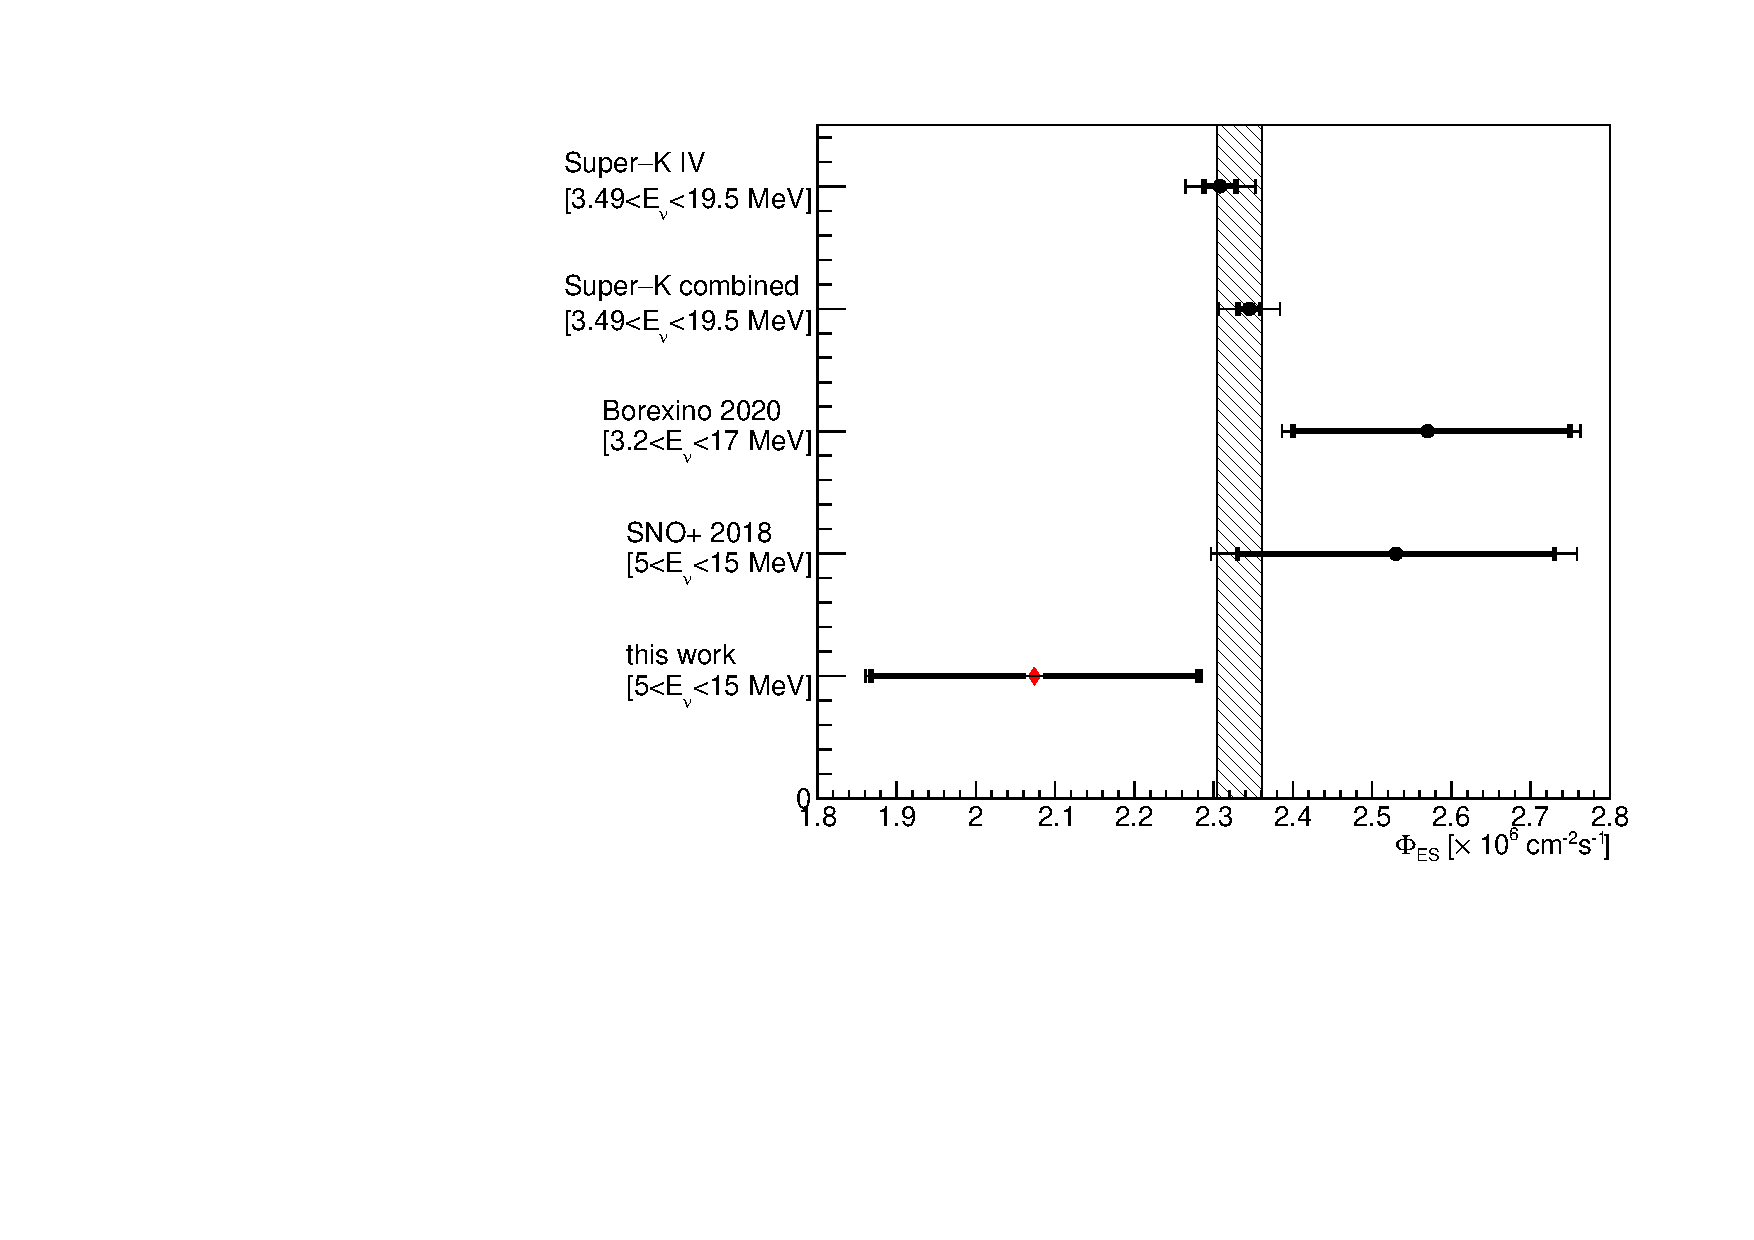
\includegraphics[width=12cm]{ESfluxCompare.pdf}
	\caption[A comparison of the ES flux measured recently by three independent experiments (after BDT selection).]{A comparison of the ES fluxes measured recently by three independent experiments (after BDT selection). The thick error bars include the statistical errors and the thin ones are quadratic errors including both the statistical and systematical errors. The shaded area is for the unconstrained average value and uncertainty: $\hat \theta \pm \sigma_{\hat \theta}$.}
	\label{fig:ESfluxCompareBDT}
\end{figure}

To combine these measurements, the unconstrained average value $\hat \theta$ and uncertainty $\sigma_{\hat\theta}$ from independent experiments are calculated by\cite{pdg2020,behnke2013data}:
\begin{equation}
\hat \theta = \sum_{i=1}^{N} \left(\frac{x_i}{\sigma_i^2}\right)\Biggm/\sum_{i=1}^{N}\left(\frac{1}{\sigma_i^2}\right),
\end{equation}
\begin{equation}
\sigma_{\hat\theta} = \sum_{i=1}^{N}\left(\frac{1}{\sigma_i^2}\right),
\end{equation}
where $x_i$ is the measured $\Phi_{ES}$ value from each experiment, and the quadratic error $\sigma_i$ is calculated by using the larger uncertainties from each experiment: $\sigma^i_{tot}=\sqrt{\sigma^2_{stat,larger}+\sigma^2_{sys,larger}}$.

If not including the value from this work, the average result is $(2.338 \pm 0.02868)\times  10^6~\mathrm{cm^{-2}s^{-1}}$. After including this work, the average result is  
$(2.333\pm0.02843)\times 10^6~\mathrm{cm^{-2}s^{-1}}$. The region of $\hat \theta\pm\sigma_{\hat\theta,tot}$ is plotted as the shaded area in Fig.~\ref{fig:ESfluxCompareBDT}.

%\begin{figure}[!htb]
%	\centering
%	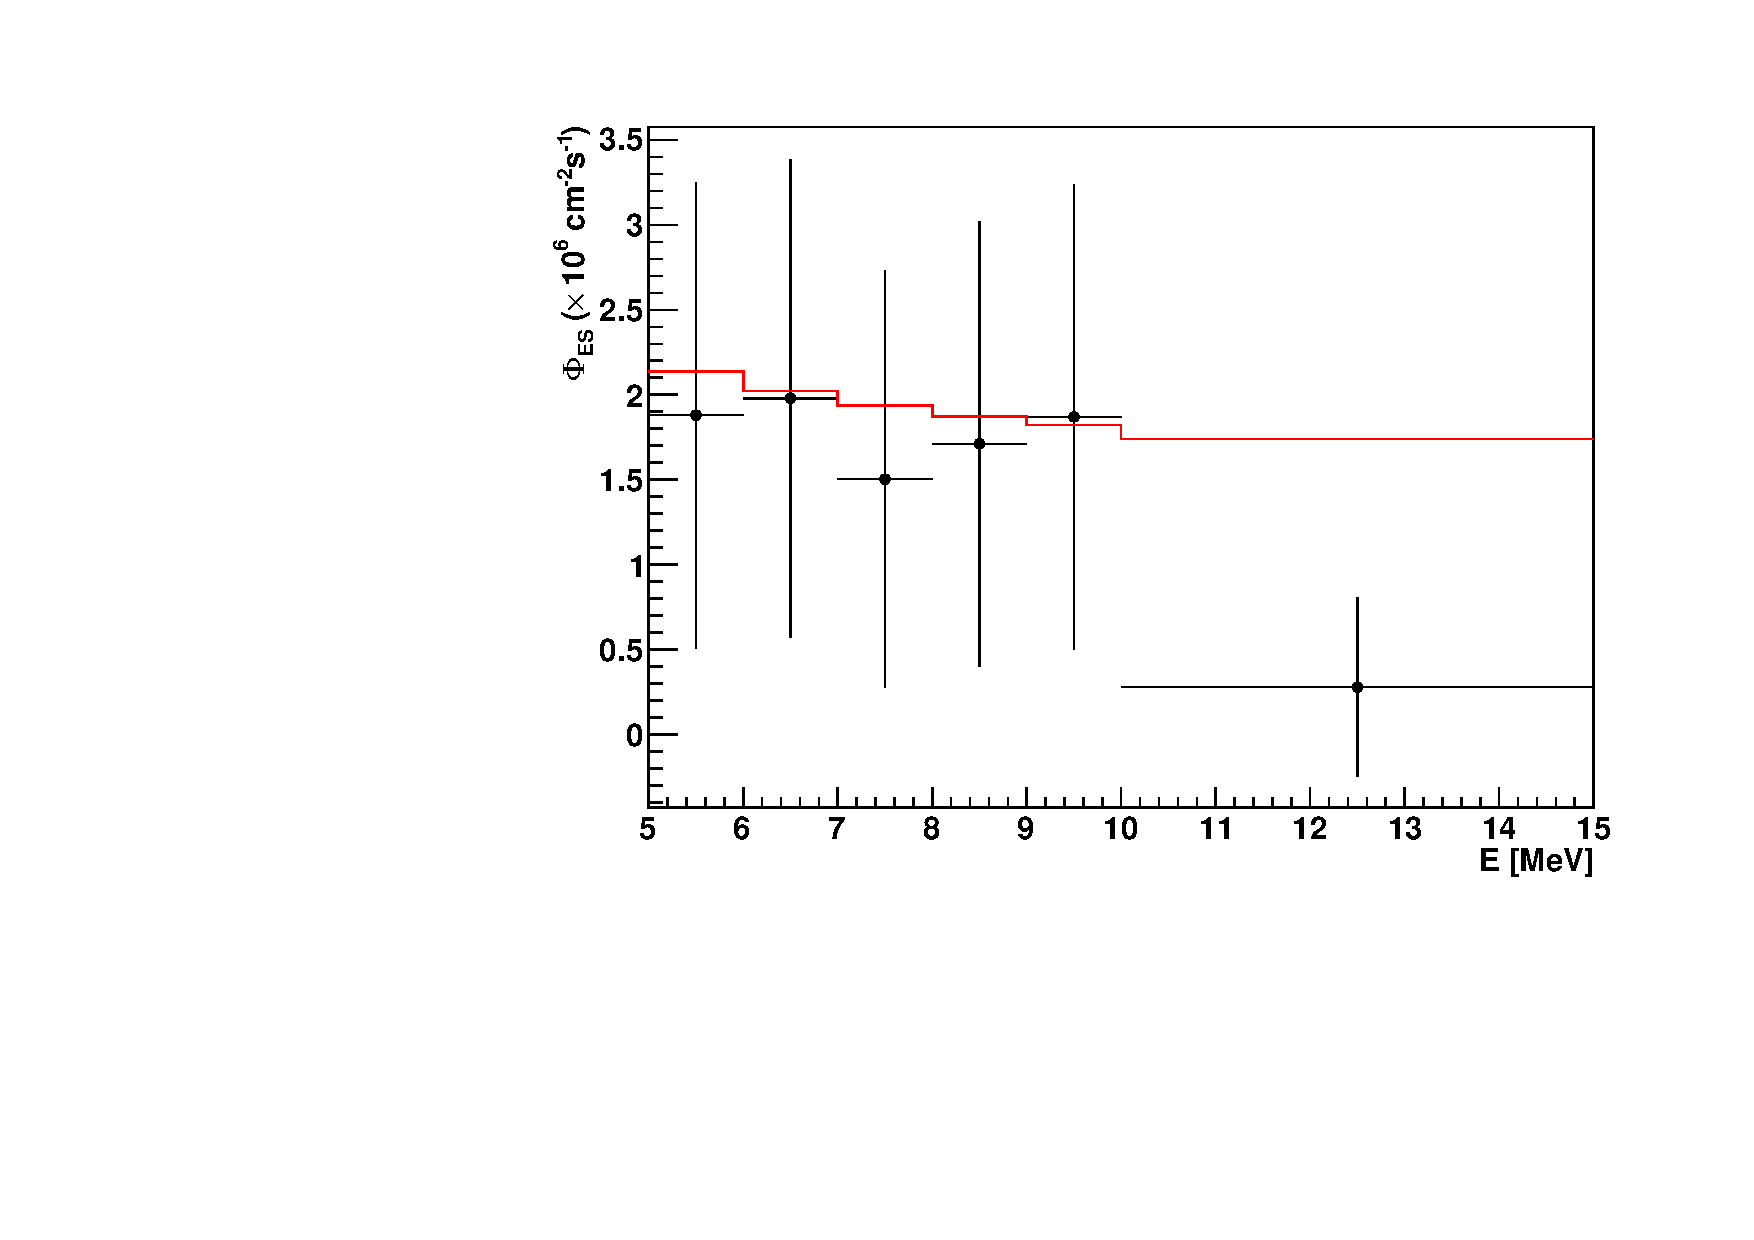
\includegraphics[width=10cm]{fluxVsEnergy.pdf}
%	\caption{$^8B$ solar neutrino flux as a function of energies. The $P_{ee}$ curve obtained from the \texttt{RAT} is in red.}
%	\label{fig:fluxVsE}
%\end{figure}

%\begin{figure}[!htb]
%	\centering
%	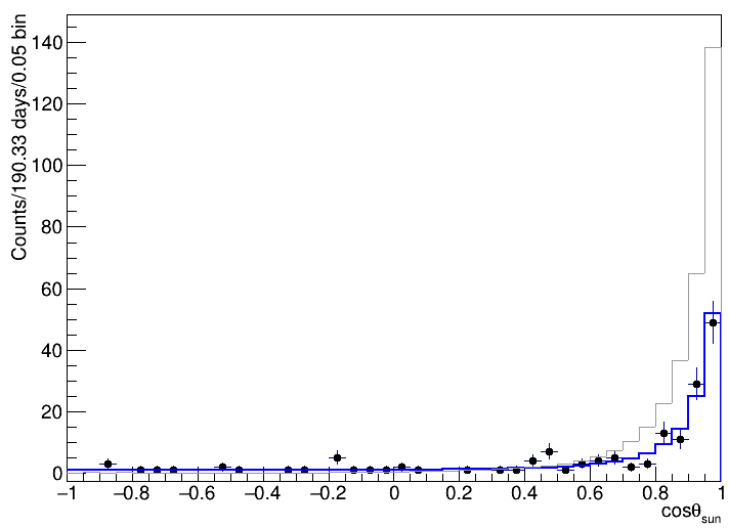
\includegraphics[width=8cm]{ESfluxFit.png}
%	\caption{$^8B$ solar neutrino flux as a function of energies. The $P_{ee}$ curve obtained from the \texttt{RAT} is in red.}
%	\label{fig:fluxVsE}
%\end{figure}

\subsubsection{Limitations of this Study}
Here I used the background types descried in the Table.~\ref{table:mixed_MC}, which were not complete. There were a few other backgrounds, such as the backgrounds from the AV ropes, the PMTs and the cosmic muon induced isotopes. A more comprehensive study requires to include all possible backgrounds.

For the background events, I assumed a flat distribution of $\cos\theta_{sun}$. A more realistic shape of the distribution can be investigated to describe the backgrounds more properly.

For the whole period of data, I used the same cuts to remove the backgrounds, while the background level can vary over time and thus require different cuts for different time periods. A more detailed description of the backgrounds over time can make the results more accurate.

Since the dataset used here has a very low background level, it is also possible to probe the energy region down to 3.5 MeV and then enable the study of the solar neutrinos in the lower energy region. This part is not included in the thesis while it is worthwhile to be investigated, especially to check the TMVA method for reducing the backgrounds in the lower energy region.